%%%%%%%%%%%%%%%%%%%%%%%%%%%%%%%%%%%%%%%%%
% kaobook
% LaTeX Class
% Version 0.9.8 (2021/08/23)
%
% This template originates from:
% https://www.LaTeXTemplates.com
%
% For the latest template development version and to make contributions:
% https://github.com/fmarotta/kaobook
%
% Authors:
% Federico Marotta (federicomarotta@mail.com)
% Based on the doctoral thesis of Ken Arroyo Ohori (https://3d.bk.tudelft.nl/ken/en)
% and on the Tufte-LaTeX class.
% Modified for LaTeX Templates by Vel (vel@latextemplates.com)
%
% License:
% LPPL (see included MANIFEST.md file)
%
% Personal modifications
% Layout / style changes to the template
% - Custom font (based on TheoWinterhalter-PhD)
% - b5paper
% - 9pt font size
%
%%%%%%%%%%%%%%%%%%%%%%%%%%%%%%%%%%%%%%%%%


%----------------------------------------------------------------------------------------
%	EXAMPLE AND DOCUMENTATION OF THE KAOBOOK CLASS
%----------------------------------------------------------------------------------------

\documentclass[
    letterpaper, % Page size
    fontsize=9pt, % Base font size
    twoside=true, % Use different layouts for even and odd pages (in particular, if twoside=true, the margin column will be always on the outside)
	% open=any, % If twoside=true, uncomment this to force new chapters to start on any page, not only on right (odd) pages
	%chapterentrydots=true, % Uncomment to output dots from the chapter name to the page number in the table of contents
	numbers=noenddot, % Comment to output dots after chapter numbers; the most common values for this option are: enddot, noenddot and auto (see the KOMAScript documentation for an in-depth explanation)
	fontmethod=modern, % Can also use "modern" with XeLaTeX or LuaTex; "tex" is the default for PdfLaTex, and "modern" is the default for those two.
]{kaobook}

%----------------------------------------------------------------------------------------
%	PACKAGES AND OTHER DOCUMENT CONFIGURATIONS
%----------------------------------------------------------------------------------------

% Choose the language
\ifxetexorluatex
	\usepackage{polyglossia}
	\setmainlanguage{english}
\else
	\usepackage[english]{babel} % Load characters and hyphenation
\fi
\usepackage[english=british]{csquotes}	% English quotes

% Load packages for testing
\usepackage{blindtext} % Print text without any meaning for testing purposes
%\usepackage{showframe} % Uncomment to show boxes around the text area, margin, header and footer
%\usepackage{showlabels} % Uncomment to output the content of \label commands to the document where they are used

% Load the bibliography package
\usepackage{kaobiblio}
\addbibresource{main.bib} % Bibliography file

% Load mathematical packages for theorems and related environments
\usepackage[framed=true]{kaotheorems}

% Load the package for hyperreferences
\usepackage{kaorefs}

\graphicspath{{examples/documentation/images/}{images/}{figures/}} % Paths in which to look for images

\makeindex[columns=3, title=Alphabetical Index, intoc] % Make LaTeX produce the files required to compile the index

\makeglossaries % Make LaTeX produce the files required to compile the glossary
\newglossaryentry{computer}{
	name=computer,
	description={is a programmable machine that receives input, stores and manipulates data, and provides output in a useful format}
}
\newglossaryentry{hybrid-cooling-system}{
	name=hybrid cooling system,
	description={integrates the dry and wet cooling systems into the same
	cooling device}
}
\newglossaryentry{combined-cooling-system}{
	name=Combined cooling system,
	description={combines separate dry and wet cooling systems within the same hydraulic circuit}
}

% How to use:
% \gls{fpsLabel} → default singular
% \glspl{fpsLabel} → plural abbreviation (e.g., FPSs)
% \gls[format=long]{fpsLabel} → singular full form (e.g., Frame per Second)
% \glspl[format=long]{fpsLabel} → plural full form (e.g., Frames per Second)


% Glossary entries (used in text with e.g. \acrfull{fpsLabel} or \acrshort{fpsLabel})
\newacronym[longplural={Frames per Second}]{fpsLabel}{FPS}{Frame per Second}
\newacronym[longplural={Tables of Contents}]{tocLabel}{TOC}{Table of Contents}
\newacronym[]{psaLabel}{PSA}{Plataforma Solar de Almería}
\newacronym[longplural={Wet Cooling Towers}]{wctLabel}{WCT}{Wet Cooling Tower}
\newacronym[]{dcLabel}{DC}{Dry Cooler}
\newacronym[]{acheLabel}{ACHE}{Air-Cooled Heat Exchanger}
\newacronym[]{cspLabel}{CSP}{Concentrated Solar Power}
\newacronym[]{annLabel}{ANN}{Artificial Neural Network}
\newacronym[]{ffLabel}{FF}{Feed Forward}
\newacronym[]{cfLabel}{CF}{Cascade-forward}
\newacronym[]{rbfLabel}{RBF}{Radial Basis Function}
\newacronym[]{ccLabel}{CC}{Combined Cooler}
\newacronym[]{ccsLabel}{CCS}{Combined Cooling System}
\newacronym[]{mimoLabel}{MIMO}{Multiple Inputs Multiple Outputs}
\newacronym[]{mseLabel}{MSE}{Mean Squared Error}
\newacronym[]{maeLabel}{MAE}{Mean Absolute Error}
\newacronym[]{rmseLabel}{RMSE}{Root Mean Squared Error}
\newacronym[]{mapeLabel}{MAPE}{Mean Absolute Percentage Error}
\newacronym[]{mreLabel}{MRE}{Mean Relative Error}
\newacronym[]{saLabel}{SA}{Sensitivity Analysis}
\newacronym[]{medLabel}{MED}{Multi-Effect Distillation}
\newacronym[
    description={A system that uses a combination of a thermal solar field and a thermal storage system as heat source to produce separation using a multi-effect distillation system.}
]{solarmedLabel}{SolarMED}{Solar-driven Multi-Effect Distillation}
\newacronym[]{sfLabel}{SF}{Solar Field}
\newacronym[]{tsLabel}{TS}{Thermal Storage}
\newacronym[]{nlpLabel}{NLP}{Non-Linear Programming}
\newacronym[]{minlpLabel}{MINLP}{Mixed Integer Non-Linear Programming}
\newacronym[]{nnlpLabel}{nNLP problems}{n Non-Linear Programming problems}
\newacronym[]{roLabel}{RO}{Reverse Osmosis}
\newacronym[]{accLabel}{ACC}{Air-Cooled Condenser}
\newacronym[]{scLabel}{SC}{Surface Condenser}
\newacronym[]{ntuLabel}{NTU}{Number of Transfer Units}
 % Include the glossary definitions
\makenomenclature % Make LaTeX produce the files required to compile the nomenclature

% Reset sidenote counter at chapters
%\counterwithin*{sidenote}{chapter}

%----------------------------------------------------------------------------------------
%	PERSONAL MODIFICATIONS
%----------------------------------------------------------------------------------------

% \usepackage{amsmath, amssymb, algorithm, algpseudocode}

\usepackage{subfig} % For subfigures
\usepackage{qrcode}
% \usepackage{fancyqr}
\usepackage{fontspec}
\usepackage{etoolbox}
\usepackage[percent]{overpic}
\newsavebox\captionqr

% Set custom font, from TheoWinterhalter-PhD
\setmainfont[
	Ligatures=TeX,
	% UprightFont = ,
	ItalicFont = Fira Sans Light Italic,
	% SmallCapsFont = ,
	BoldFont = Fira Sans,
	BoldItalicFont = Fira Sans Italic
	]{Fira Sans Light}
\setsansfont[Ligatures=TeX]{Fira Sans}
\setmonofont[Ligatures=TeX]{Fira Mono}

% Customising margin citations, from TheoWinterhalter-PhD
\renewcommand{\formatmargincitation}[1]{%
\color{Gray!90} \parencite{#1}: \citeauthor*{#1} (\citeyear{#1}), \citetitle{#1}\\%
}

% Set some mathematical operators
\DeclareMathOperator{\lew}{Le}
\DeclareMathOperator{\Me}{Me}

% Define the base URL for the figures repository
% Used for QR codes to link to the interactive version of some figures
\newcommand{\repositoryBaseUrl}{https://github.com/juan11iguel/my-thesis/blob/main} % Replace with your actual ID

% TODO: Move into macros.tex
% Reminder box
% \newcommand{\reminder}[3][0pt]{%
%   \marginnote[#1]{%
%     \begin{kaobox}[
%     %   title=Reminder: #2,
%     %   colback=YellowGreen!25!white,
%     %   colbacktitle=YellowGreen!25!white,
%     %   colframe=black,
%     %   fonttitle=\bfseries,
%     %   titlerule=0.4pt
%     ]
%       #3
%     \end{kaobox}
%   }%
% }
\newcommand{\marginreminder}[3][0pt]{%
  \marginnote[#1]{%
    \begingroup
      \edef\tempTitle{Reminder: #2}%
      \begin{kaobox}[title=\tempTitle,
        colback=YellowGreen!25!white,
        colbacktitle=YellowGreen!25!white,
        colframe=black,
        fonttitle=\bfseries,
        titlerule=0.4pt
      ]
        #3
      \end{kaobox}
    \endgroup
  }%
}

\newcommand{\reminder}[2]{%
  \begingroup
    \edef\tempTitle{Reminder: #1}%
    \begin{kaobox}[title=\tempTitle,
      colback=YellowGreen!25!white,
      colbacktitle=YellowGreen!25!white,
      colframe=black,
      fonttitle=\bfseries,
      titlerule=0.4pt
    ]
      #2
    \end{kaobox}
  \endgroup
}

\newcommand{\tldrbox}[1]{%
    \begin{kaobox}[title=TL;DR,
      colback=Orchid!25!white,
      colbacktitle=Orchid!25!white,
    %   colframe=black,
      fonttitle=\bfseries,
      titlerule=0.05pt
    ]
	#1
    \end{kaobox}
}

% TODO: This should be a box with a counter so it can be referenced
\newcommand{\problemdefinitionbox}[2]{%
  \begingroup
    \edef\tempTitle{Problem: #1}%
    \begin{kaobox}[title=\tempTitle,
      colback=Snow3!25!white,
      colbacktitle=Snow3!25!white,
    ]
	#2
    \end{kaobox}
  \endgroup
}

\newcommand{\fullgls}[1]{\gls[format=long]{#1}}

%----------------------------------------------------------------------------------------

\begin{document}

\begin{modelcounter}{Test}
	\begin{align*}
    T_{cc,out},\,C_{e}&,\,C_{w},\,T_{c,out} = \mathrm{combined\:cooler\:model}(q_{c}, R_{p}, R_{s}, \omega_{dc}, \omega_{wct},T_{amb},HR_i,T_{v},\dot{m}_{v}) \\
    & T_{cc,in}=T_{c,out} \\
    & T_{dc,in}=T_{cc,in} \\
    % three-way valves
    & q_{dc} = q_{c} \cdot (1-R_{p}) \\
    & q_{wct,p} = q_{c} \cdot R_{p} \\
    & q_{wct,s} = q_{dc} \cdot R_{s} \\
    % dc model
    & T_{dc,out},\,C_{e,dc} = \mathrm{dc\:model}(q_{dc},\, \omega_{\text{dc}},\, T_{\text{amb}},\, T_{dc,in}) \\
    % first mixer
    & q_{wct},\,T_{wct,in} = \mathrm{mixer\:model}(q_{wct,p},\,T_{T{cc,in}},\, q_{wct,s},\, T_{dc,out}) \\
    % wct model
    & T_{wct,out},\,C_{e,wct},\,C_{w,wct} = \mathrm{wct\:model}(q_{wct},\, \omega_{wct},\, T_{amb},\, HR,\, T_{wct,in}) \\
    % condenser model
    & T_{c,in},\,T_{c,out} = \mathrm{condenser\:model}(q_c,\, \dot{m}_v,\, T_v) \\
    % final mixer
    & q_{cc},\,T_{cc,out} = \mathrm{mixer\:model}(q_{wct},\, T_{wct,out},\, q_{dc},\, T_{dc,out}) \\
    % totals
    & C_{e} = C_{e,dc} + C_{e,wct} + C_{e,c} \\
    & C_{w} = C_{w,wct}
    \end{align*}
	\labmod{test}
\end{modelcounter}

As can be seen in \refmod{test}, the counter is working.

\begin{problemcounter}{Test}
	\blindtext
  \begin{equation*}
	\min_{\mathbf{x},\, \mathbf{e};\, \boldsymbol{\theta}} \quad J = f(\mathbf{x}, \mathbf{e}; \boldsymbol{\theta}) = f(x)
  \end{equation*}

  \textbf{with}:
  \begin{itemize}
	\item Model name model
	\[
	  out_1,\, out_2 = f(in_1,\, in_2,\, \ldots,\, in_N)
	\]
	\item Decision variables
	\[
	  \mathbf{x} = [x_1,\, x_2]
	\]
	\item Environment variables
	\[
	  \mathbf{e} = [e_1,\, e_2,\, \ldots,\, e_3]
	\]
	\item Fixed parameters
	\[
	  \boldsymbol{\theta} = [\theta_1 = X,\, \theta_2 = Y]
	\]
  \end{itemize}

  \textbf{subject to}:
  \begin{itemize}
	\item Box-bounds
	\begin{itemize}
	  \item \( x_{1} \in [\underline{x}_{1}, \overline{x}_{1}] \)
	  \item \( x_{2} \in [\underline{x}_{2}, \overline{x}_{2}] \)
	\end{itemize}
	\item Constraints
	\begin{itemize}
	  \item \( \left| out_X - out_Y \right| \leq \epsilon_1 \)
	  \item \( out_X \leq out_Z - \Delta Z \)
	\end{itemize}
  \end{itemize}
  \labprob{test}
\end{problemcounter}

As can be seen in \refprob{test}, the counter is working.

\tldrbox{test test}
% \blindtext\blindtext

\problemdefinitionbox{Test}{
  \begin{equation*}
	\min_{\mathbf{x},\, \mathbf{e};\, \boldsymbol{\theta}} \quad J = f(\mathbf{x}, \mathbf{e}; \boldsymbol{\theta}) = f(x)
  \end{equation*}

  \textbf{with}:
  \begin{itemize}
	\item Model name model
	\[
	  out_1,\, out_2 = f(in_1,\, in_2,\, \ldots,\, in_N)
	\]
	\item Decision variables
	\[
	  \mathbf{x} = [x_1,\, x_2]
	\]
	\item Environment variables
	\[
	  \mathbf{e} = [e_1,\, e_2,\, \ldots,\, e_3]
	\]
	\item Fixed parameters
	\[
	  \boldsymbol{\theta} = [\theta_1 = X,\, \theta_2 = Y]
	\]
  \end{itemize}

  \textbf{subject to}:
  \begin{itemize}
	\item Box-bounds
	\begin{itemize}
	  \item $x_{1} \in [\underline{x}_{1}, \overline{x}_{1}]$
	  \item $x_{2} \in [\underline{x}_{2}, \overline{x}_{2}]$
	\end{itemize}
	\item Constraints
	\begin{itemize}
	  \item $\left| out_X - out_Y \right| \leq \epsilon_1$
	  \item $out_X \leq out_Z - \Delta Z$
	\end{itemize}
  \end{itemize}
}


% \marginreminder{Pareto front}{
% When dealing with multiple objectives where no single solution is optimal, but
% improvements in one objective lead to trade-offs in others, we obtain a set of
% points that represent the best trade-offs between the objectives, known as a
% Pareto front\footnote{See \nrefsec{intro:optimization:multi-objective}}
% }

% \section*{Two-Level Pareto Path Optimization}

% We consider a complex optimization problem over a prediction horizon of length $N$. At each stage $t = 1, \dots, N$, we define and solve a multi-objective optimization problem:

% \[
% \text{Find } \mathcal{P}_t = \text{ParetoFront}(f_t(x_t)), \quad x_t \in \mathcal{X}_t
% \]

% where $f_t : \mathcal{X}_t \rightarrow \mathbb{R}^k$ defines $k$ objectives at stage $t$. The result is a set of Pareto-optimal solutions $\mathcal{P}_t$.

% The second-level problem seeks a sequence of decisions $(x_1^*, \dots, x_N^*)$ with $x_t^* \in \mathcal{P}_t$ that minimizes a cumulative cost function:

% \[
% \min_{x_1 \in \mathcal{P}_1, \dots, x_N \in \mathcal{P}_N} \sum_{t=1}^{N-1} c(x_t, x_{t+1}) + \sum_{t=1}^{N} g(x_t)
% \]

% where $c(x_t, x_{t+1})$ encodes transition costs and $g(x_t)$ may represent stage-specific penalties.

% \bigskip

% \begin{algorithm}[H]
% \caption{Two-Level Pareto Path Optimization}
% \begin{algorithmic}[1]
% \State \textbf{Input:} Horizon length $N$
% \For{$t = 1$ to $N$}
%     \State Solve multi-objective optimization at stage $t$ to get Pareto set $\mathcal{P}_t$
% \EndFor
% \State Define graph $\mathcal{G}$ with layers $\mathcal{P}_1, \dots, \mathcal{P}_N$
% \State Add edges between layers: connect each $x_t \in \mathcal{P}_t$ to all $x_{t+1} \in \mathcal{P}_{t+1}$ with weight $c(x_t, x_{t+1})$
% \State Solve shortest path or path optimization on $\mathcal{G}$ to find optimal path $(x_1^*, \dots, x_N^*)$
% \State \textbf{Return} path and corresponding objective values
% \end{algorithmic}
% \end{algorithm}

%----------------------------------------------------------------------------------------
%	BOOK INFORMATION
%----------------------------------------------------------------------------------------

\titlehead{The \texttt{kaobook} class}
\subject{PhD Thesis}

\title[Towards optimal resource management in solar thermal applications]{Towards optimal resource management in solar thermal applications: desalination and CSP}
% \subtitle{Customise this page according to your needs}

\author[Juan Miguel Serrano]{Juan Miguel Serrano Rodríguez}
\date{\today}

\publishers{University of Almería}

%----------------------------------------------------------------------------------------

\frontmatter % Denotes the start of the pre-document content, uses roman numerals

%----------------------------------------------------------------------------------------
%	OPENING PAGE
%----------------------------------------------------------------------------------------

% \makeatletter
% \extratitle{
% 	% In the title page, the title is vspaced by 9.5\baselineskip
% 	\vspace*{9\baselineskip}
% 	\vspace*{\parskip}
% 	\begin{center}
% 		% In the title page, \huge is set after the komafont for title
% 		\usekomafont{title}\huge\@title
% 	\end{center}
% }
% \makeatother

%----------------------------------------------------------------------------------------
%	COPYRIGHT PAGE
%----------------------------------------------------------------------------------------

\makeatletter
\uppertitleback{\@titlehead} % Header

\lowertitleback{
	\textbf{Disclaimer}\\
	You can edit this page to suit your needs. For instance, here we have a no copyright statement, a colophon and some other information. This page is based on the corresponding page of Ken Arroyo Ohori's thesis, with minimal changes.
	
	\medskip
	
	\textbf{No copyright}\\
	\cczero\ This book is released into the public domain using the CC0 code. To the extent possible under law, I waive all copyright and related or neighbouring rights to this work.
	
	To view a copy of the CC0 code, visit: \\\url{http://creativecommons.org/publicdomain/zero/1.0/}
	
	\medskip
	
	\textbf{Colophon} \\
	This document was typeset with the help of \href{https://sourceforge.net/projects/koma-script/}{\KOMAScript} and \href{https://www.latex-project.org/}{\LaTeX} using the \href{https://github.com/fmarotta/kaobook/}{kaobook} class.
	
	The source code of this book is available at:\\\url{https://github.com/fmarotta/kaobook}
	
	(You are welcome to contribute!)
	
	\medskip
	
	\textbf{Publisher} \\
	First printed in May 2019 by \@publishers
}
\makeatother

%----------------------------------------------------------------------------------------
%	DEDICATION
%----------------------------------------------------------------------------------------

\dedication{
	The harmony of the world is made manifest in Form and Number, and the heart and soul and all the poetry of Natural Philosophy are embodied in the concept of mathematical beauty.\\
	\flushright -- D'Arcy Wentworth Thompson
	% \flushleft - ¿Quieres que te cuente el cuento del rábano pimiento? \\
	% \flushright - ¡Vale! \\
	% \flushleft - No te he preguntado si \textit{vale}, te he preguntado que si\\ quieres 
	% que te cuente el cuento del rábano pimiento. \\
	% \flushright-Sí, una vez más, por favor. \\
	% \vspace{5ex}
	% \flushleft\textit{Un abuelo y su nieto}
}

%----------------------------------------------------------------------------------------
%	OUTPUT TITLE PAGE AND PREVIOUS
%----------------------------------------------------------------------------------------

% Note that \maketitle outputs the pages before here

\maketitle

%----------------------------------------------------------------------------------------
%	PREFACE
%----------------------------------------------------------------------------------------

\chapter*{Acknowledgements}
\addcontentsline{toc}{chapter}{Acknowledgements}

Test test test
% To my family, if you did  not ask about how was I doing with the thesis, every
% single time you saw me, I might have forgotten I had to actually finish it.

\begin{flushright}
	\textit{Federico Marotta}
\end{flushright}


\chapter*{Summary}
\addcontentsline{toc}{chapter}{Summary} % Add the preface to the table of contents as a chapter

I am of the opinion that every \LaTeX\xspace geek, at least once during 
his life, feels the need to create his or her own class: this is what 
happened to me and here is the result, which, however, should be seen as 
a work still in progress. Actually, this class is not completely 
original, but it is a blend of all the best ideas that I have found in a 
number of guides, tutorials, blogs and tex.stackexchange.com posts. In 
particular, the main ideas come from two sources:

\begin{itemize}
	\item \href{https://3d.bk.tudelft.nl/ken/en/}{Ken Arroyo Ohori}'s 
	\href{https://3d.bk.tudelft.nl/ken/en/nl/ken/en/2016/04/17/a-1.5-column-layout-in-latex.html}{Doctoral 
	Thesis}, which served, with the author's permission, as a backbone 
	for the implementation of this class;
	\item The 
		\href{https://github.com/Tufte-LaTeX/tufte-latex}{Tufte-Latex 
			Class}, which was a model for the style.
\end{itemize}

The first chapter of this book is introductory and covers the most
essential features of the class. Next, there is a bunch of chapters 
devoted to all the commands and environments that you may use in writing 
a book; in particular, it will be explained how to add notes, figures 
and tables, and references. The second part deals with the page layout 
and design, as well as additional features like coloured boxes and 
theorem environments.

I started writing this class as an experiment, and as such it should be 
regarded. Since it has always been intended for my personal use, it may
not be perfect but I find it quite satisfactory for the use I want to 
make of it. I share this work in the hope that someone might find here 
the inspiration for writing his or her own class.

\chapter*{Resumen}
\addcontentsline{toc}{chapter}{Resumen}



\chapter*{How to read this thesis}
\addcontentsline{toc}{chapter}{How to read this thesis}


% I believe that a document of this size will be more often viewed on computer
% than on paper. This how I personally view most papers I read anyway.
% As such, I believe that the document should be adapted for such a medium, unlike
% most \LaTeX{} documents.
% While trying to make my own kind of document, I stumbled upon the great
% \href{https://github.com/fmarotta/kaobook/}{kaobook} class which corresponds
% almost exactly to what I was looking for: citations, notes, reminders can be put
% in a large margin.

% Citations like~\sidecite{KOMAScriptDoc} will go in the
% margin, as well as in the \refbib.
% The margin also contain side notes\sidenote{
%   No more going back and forth between the end and top of the page.
% }, replacing the usual footnotes.

% I will also use margin notes that are not anchored in the main document but are
% usually relevant to the paragraph or figure on their left.
% \marginnote[-0.4cm]{
%   Margin notes are not placed entirely automatically. I tend to adjust the
%   height so it is at the right place.
% }

% \begin{theorem}
%   Theorems and definitions will be in these yellow boxes.
% \end{theorem}

% On the other hand, I will sometimes refer to concepts for the first time without
% taking the time to introduce them because they are secondary to the main point.
% In some cases those will be accompanied by a short definition on the side, in
% a yellowish box.

\chapter*{About the author}
\addcontentsline{toc}{chapter}{About the author}

% Un payaso\\ \flushright{-- Lidia Roca, probablemente}
\index{preface}

%----------------------------------------------------------------------------------------
%	TABLE OF CONTENTS & LIST OF FIGURES/TABLES
%----------------------------------------------------------------------------------------

\begingroup % Local scope for the following commands

% Define the style for the TOC, LOF, and LOT
%\setstretch{1} % Uncomment to modify line spacing in the ToC
%\hypersetup{linkcolor=blue} % Uncomment to set the colour of links in the ToC
\setlength{\textheight}{230\hscale} % Manually adjust the height of the ToC pages

% Turn on compatibility mode for the etoc package
\etocstandarddisplaystyle % "toc display" as if etoc was not loaded
\etocstandardlines % "toc lines as if etoc was not loaded

\tableofcontents % Output the table of contents

\listoffigures % Output the list of figures

% Comment both of the following lines to have the LOF and the LOT on 
% different pages
\let\cleardoublepage\bigskip
\let\clearpage\bigskip

\listoftables % Output the list of tables

\listoflstlistings % Output the list of listings

% TODO: Add \listofcontributions

\endgroup


% \chapter*{How to read this thesis}
\addcontentsline{toc}{chapter}{How to read this thesis}

\tldrbox{
    This preliminary chapter explains how to read this thesis, mainly the
    different environment boxes used throughout the manuscript, why the large
    margins, what is placed in them, and how to use the interactive features
    of the manuscript. This is an example of a \gls{tldrLabel} box. It contains
    an Abstract/Summary of the main point of the chapter and are placed at the
    beginning of every chapter.
}

This \LaTeX{} template is designed with large margins, on the one hand this
allows to have shorter lines, which makes for an easier reading experience but
most interestingly, it also allows to place additional information in the
margins, such as side notes, side citations, figures, tables… your
imagination is the limit! Or rather \LaTeX{} compilation errors and your
patience are. Throughout this manuscript I will add side notes\sidenote{
  Like this one! They are like footnotes, but placed in the margin of the page
} to provide additional information and comments that would otherwise be too
distracting and verbose to include in the main text, constantly interrupting
the flow of the reading. The side notes are not essential to understand the
content of the document, but mostly complementary.

\section*{Boxed environments}

Both problem definition boxes (\eg ref) and model definition boxes (\eg
\refmod{example}) are countered environments and can (and will) be referenced
in the text.

\begin{marginfigure}[]
    \includegraphics[]{figures/WASCOP-facility-WCT.png}
    % \caption{Back view of the WCT}
    \savebox\captionqr{\qrcode[hyperlink,height=0.4in]{\repositoryBaseUrl/figures/day_viz_20220614_eval_at_20250414T1247_test_water_price.html}}
    % \caption{\parbox{0.8\textwidth}{Line 1 of caption\\Line 2 of caption}}
	\caption{Example figure. Try clicking or scanning the QR code to access the
	interactive version.\\[1ex]\usebox\captionqr}
    \labfig{how-to-read:example-figure}
\end{marginfigure}


\problemdefinitionbox{Problem definition box example}{
    This is an example of a problem definition box. It is used to formally and
    concisely define an optimization problem.
  \begin{equation*}
    \min_{\mathbf{x},\, \mathbf{e};\, \boldsymbol{\theta}} \quad J = f(\mathbf{x}, \mathbf{e}; \boldsymbol{\theta}) = XXXX
  \end{equation*}

  \textbf{with}:
  \begin{align*}
      out_1,\, out_2 &= f(in_1,\, in_2,\, \ldots,\, in_N)\\
      out_1,\, out_2 &= f(in_1,\, in_2,\, \ldots,\, in_N)
  \end{align*}
  \begin{itemize}
    \item Decision variables
    \[
      \mathbf{x} = [x_1,\, x_2]
    \]
    \item Environment variables
    \[
      \mathbf{e} = [e_1,\, e_2,\, \ldots,\, e_3]
    \]
    \item Fixed parameters
    \[
      \boldsymbol{\theta} = [\theta_1 = X,\, \theta_2 = Y]
    \]
  \end{itemize}

  \textbf{subject to}:
  \begin{itemize}
    \item Box-bounds
    \begin{itemize}
      \item $x_{1} \in [\underline{x}_{1}, \overline{x}_{1}]$
      \item $x_{2} \in [\underline{x}_{2}, \overline{x}_{2}]$
    \end{itemize}
    \item Constraints
    \begin{itemize}
      \item $\left| out_X - out_Y \right| \leq \epsilon_1$
      \item $out_X \leq out_Z - \Delta Z$
    \end{itemize}
  \end{itemize}
}

\begin{modelcounter}{Model definition box example}
    \begin{equation*}
        out_{1},\,out_{2} = \text{some\:cool\:model}(in_{1},\, in_{2},\, in_{3})
    \end{equation*}
    \labmod{example}
\end{modelcounter}

\begin{kaobox}[title=Other boxes]
    Other boxes are used to highlight important points, or to provide
    additional information that is not essential to the main text.
\end{kaobox}

% On the other hand, I will sometimes refer to concepts for the first time without
% taking the time to introduce them because they are secondary to the main point.
% In some cases those will be accompanied by a short definition on the side, in
% a yellowish box.

In order to make the book more interactive and link-friendly, I have enabled
hyperlinks in the PDF. This means that you can click on the references,
citations, and links to external resources, and they will take you to the
corresponding location. This is standard latex, however to maintain a
consistent experience in the physical version, QR codes are inserted in the
margin next to the links. The reader is invited to scan them with a QR code
reader to access the corresponding online resource\sidenote[][*-8]{
    I believe that this is a good way to make the document more
accessible and to encourage readers to explore the content in more depth.
However, the interactive features are \textbf{optional} and not necessary to
understand the content of the document.
}. Some figures also include QR codes that link to an interactive (HTML)
version of the figure, see \reffig{how-to-read:example-figure} as an example.

The additional material as
well as the source code of this document are hosted in a \href{\repositoryBaseUrl}{Zenodo repository}\sidenote[][*-2]{
    \qrcode[hyperlink,height=0.5in]{\repositoryBaseUrl}
}. Alternatively, a mirror repository is also available at: \\
\begin{center}
    \href{https://github.com/juan11iguel/my-thesis}{https://github.com/juan11iguel/my-thesis} \\
\end{center}
It seems unlikely that both Zenodo and GitHub will go down at a time where this
document is still relevant, and if they do, I think there will be more
important things to worry about than losing access to the interactive content
of this thesis.\sidenote[{\color{gray} \faToiletPaper}]{Like hoarding toilet paper}

% \chapter*{About the author}
\addcontentsline{toc}{chapter}{About the author}

\begin{marginfigure}[]
    \includegraphics[]{figures/bussines_cat.jpg}
    % \caption{}
    % \labfig{chapter:section:bussines_cat}
\end{marginfigure}

Un payaso
\vspace{1em}
\begin{flushright}
-- Lidia Roca, probablemente
\end{flushright}


I am currently completing my PhD thesis, with the defense planned for October.
My research interests lie primarily in automatic control, optimization, and
robotics, especially as applied to solar thermal processes.

I think I am mostly a creative person, but in order to implement those ideas,
throughout my work, I’ve gained experience with a variety of tools and
technologies, including Linux, Python, Docker, LaTeX, and the Robot Operating
System (ROS). I’m particularly passionate about open science and open source
software, and I strive to contribute to communities that value transparency and
collaboration.

For my bachelor's thesis, I created a mobile robotics lab in the University of
Almería by deploying the \href{https://duckietown.com/}{Duckietown project}.
This gave me the opportunity to interact and work with ROS, and since the whole
project was deployed using Docker, to learn about containerization
technologies. For my master's thesis, work was also software-related, but this
time it was about the implementation of a SCADA-like system using Python.
During my PhD, I have had four years to really delve into these technologies,
so today they are an integral part of my workflow and I am confident to say
they've helped me become effective at implementing those (sometimes too) many
ideas\todo{Lidia esto solo lo he copiado por tener algo, ya lo mejoraré}.


%----------------------------------------------------------------------------------------
%	MAIN BODY
%----------------------------------------------------------------------------------------

\mainmatter % Denotes the start of the main document content, resets page numbering and uses arabic numbers
\setchapterstyle{kao} % Choose the default chapter heading style

%----------------------------------------------------------------------------------------
%	INTRODUCTION
%----------------------------------------------------------------------------------------
\chapter*{Preface}
\addcontentsline{toc}{chapter}{Preface}

% Sokolowski, John A., and Catherine M. Banks. Principles of Modeling and Simulation: A Multidisciplinary Approach. John Wiley & Sons, 2011.


Un par de párrafos hablando del contexto de la tesis, sobre qué trata y para qué
tipo de audiencia está dirigida.

Seguir con estructura:

The text is divided into three parts with X chapters. Part One introduces the context and motivation of the thesis, the
        research plan, and the contributions. ... 

This introductory part is then followed by the two main contributions. In Part 2
...


Part 3...



\pagelayout{wide} % No margins
\addpart{Introduction}
\pagelayout{margin} % Restore margins

\setchapterpreamble[u]{\margintoc}
\chapter{Context and motivation}
\labch{intro:context}

\blindtext\blindtext\blindtext\blindtext\blindtext
\begin{marginfigure}[-5.5cm]
    \includegraphics[]{figures/shareholders-driven-apocalysis.png}
    \caption{``Yes, the planet got destroyed. But for a beautiful moment in time, we created a lot of value for shareholders''}
    % \labfig{}
\end{marginfigure}


\blindtext\blindtext\blindtext\blindtext


\begin{figure}[htbp]
    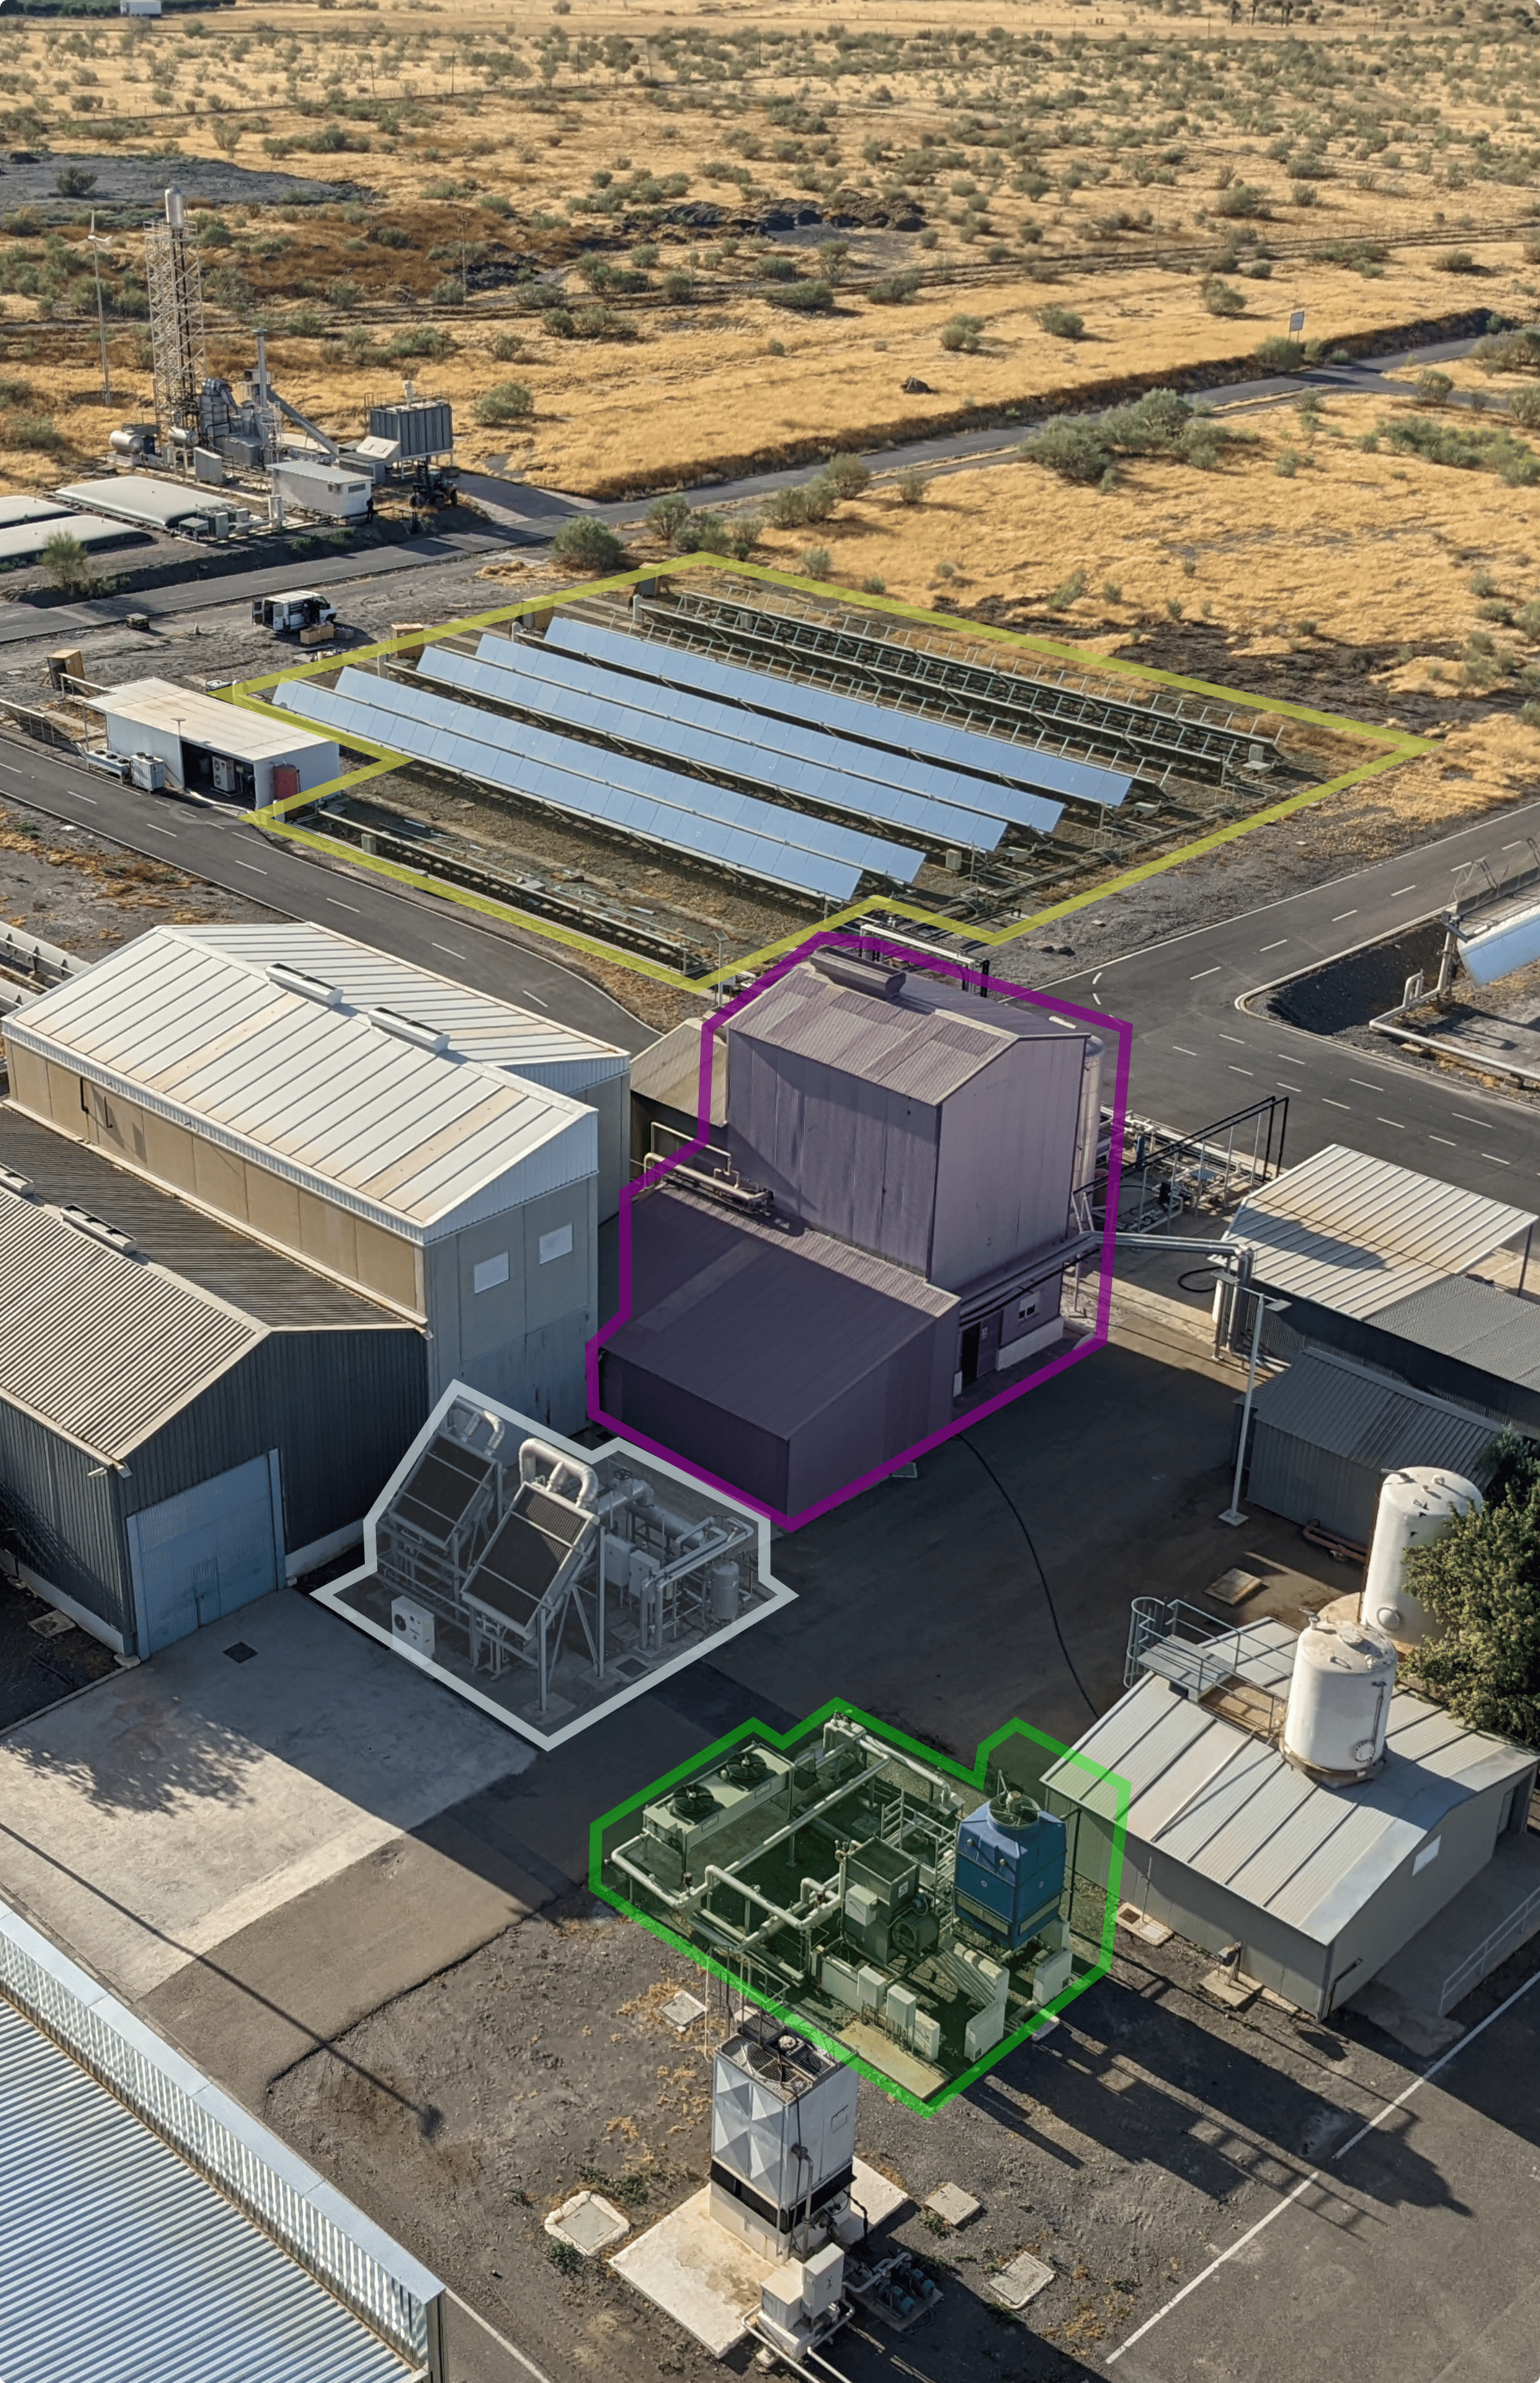
\includegraphics[width=\textwidth]{figures/pilot-plants-aerial-view.png}
    \caption{
        \textbf{Aerial view of the pilot plants at the \fullgls{psaLabel}, Spain.}\\ 
        The developments presented in this thesis have
        been developed and validated around two test-rigs: a
        \gls{ccsLabel} and a \gls{solarmedLabel} pilot plants. In the picture, the
        \gls{ccsLabel} plant is located on the left side, and the...
    }
    \labfig{intro:pilot-plants}
\end{figure}


%===================================
%===================================
%===================================
\setchapterpreamble[u]{\margintoc}
\chapter{Research plan}
\labch{intro:plan}
% Fijarse en Tesis Simon

asdad

%===================================
%===================================
\section{Hypothesis}
\labsec{intro:research-plan:hypothesis}

%===================================
%===================================
\section{Objectives}
\labsec{intro:research-plan:objectives}

%===================================
%===================================
\section{Contributions}
\labsec{intro:research-plan:contributions}


% %===================================
% %===================================
% %===================================
% \setchapterpreamble[u]{\margintoc}
% \chapter{Contributions}
% \labch{intro:contributions}

% % Generales de la tesis, abstracto
% asdad

%===================================
%===================================
%===================================
\setchapterpreamble[u]{\margintoc}
\chapter{Automation overview: modelling, optimization and control}
\labch{intro:automation}

Automation, and particularly process automation, is a multidisciplinary
technology that by integrating various fields of knowledge, aims to develop
autonomous systems, capable of operating with minimal human intervention, using
resources efficiently, adapting to changing conditions, and ensuring safety
and reliability. 

This chapter provides an overview of the main aspects of automation, focusing on
modelling, optimization and control. These three pillars are essential for the
development of advanced automation systems and are widely used in the industry.
The chapter is structured as follows: first, an overview of modelling techniques
is presented, including first-principles and data-driven approaches. Then,
optimization methods are discussed, covering both single-objective and
multi-objective optimization. Finally, control strategies are reviewed, with a
focus on PID control and hierarchical control.

\begin{kaobox}[title=Dealing with complexity]
    Real systems are complex, with many elements interconnected. We first need
    to simplify them into simpler blocks  or levels of abstraction that we can
    work with. These blocks or boxes have inputs and outputs, internally they
    hide some complexity, but from our abstraction we only care that we give
    some input to them, they perform some transformation, and then they return
    some output. These then can be interconnected to form a complex network or
    structure representing the real process. \\
    
    This layering is common in many different fields, for example, processors
    are made up by thousands of layers, with modern processors going from
    city-like structures in the upper layers while reaching atomic scales in the
    lowest layers. \\

    \begin{minipage}{0.4\linewidth}
    \centering
    \includegraphics[width=\linewidth]{figures/microprocessor-min.jpg}\\
    \small Zoomed-in microprocessor. Source: \href{https://www.reddit.com/r/interestingasfuck/comments/ksz30z/oc_i_took_an_old_intel_d320_cpu_and_torn_it_apart/}{stylishpirate - Reddit}
    \end{minipage}
    \hfill
    \begin{minipage}{0.58\linewidth}
    \centering
    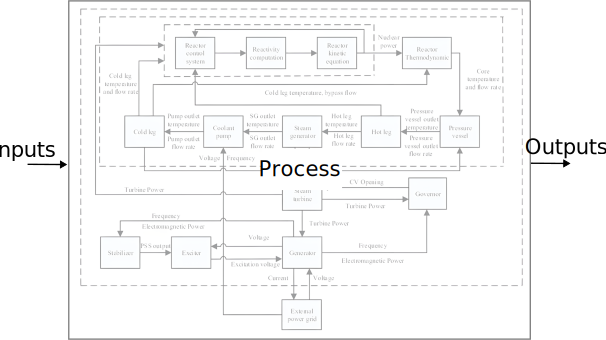
\includegraphics[width=\linewidth]{figures/block-diagram.png}\\
    \small Block diagram with input and outputs
    \end{minipage}
\end{kaobox}

%===================================
%===================================
\section{Modelling and simulation}
\labsec{intro:modelling}

%% Explicación del concepto de modelado %%
Models are  useful  approximations for the real-world
~\sidecite{sokolowski_principles_2011}, more precisely a mathematical
representation of real-world systems. A model can depict a system at different
levels of abstraction depending on the intended use. Models are useful in many
applications: 

\begin{itemize}
    \item Forecasting. They are used to predict the value of a variable at some
    time in the future. 
    \item Simulation. Oftentimes experimentally evaluating real-world systems is
    impractical or infeasible, either because it is costly it may require a lot of
    time, or deteriorate the system among other factors. Simulating a model enables
    the repeated observation of a system with just an associated computational
    cost. 
    \item Control and optimization. in order to compute the optimal input to
    give to a real system, many control strategies are model-based, that is, they
    assess how inputs given to the real system will affect it by first evaluating
    them in a model. 
    \item Analysis of models enables to draw conclusions, verify and validate
    the research, and make recommendations in order to support decision-making.
\end{itemize}

\begin{kaobox}[title=Sensitivity analysis]
    Sensitivity analysis is one of the possible analysis tools. It involves
  systematically assessing how variations in input parameters impact the model
  outputs. > One of the methods used in this research work is the Sobol
  method~\cite{nossent_sobolsensitivity_2011}, which is a variance-based
  approach. This method decomposes the total variance of the model output into
  contributions from individual input parameters and their interactions.
\end{kaobox}

%% Tipos de sistemas: dinámicos, estáticos %%
All real world systems are fundamentally dynamical systems, that is, they
evolve over time. For example a fluid flowing over a plane wing, the spread of a
disease, the climate of a planet, the stock market, planets moving around the
solar system. This behavior takes place continuously with respect to time for
most physical systems, and can be described using differential equations. An
alternative discrete representation can be achieved by performing a
transformation from the continuous space to a discrete space sampling data at
discrete time intervals and is described by difference equations. For an
infinitesimal small time interval they are equivalent. In practice, discrete
representation is a simplification of continuous systems.

An example of the position ($y$) of an object free-falling by gravity could be
represented:
\begin{itemize}
    \item In a dynamic continuous space as $\frac{d^2 y(t)}{dt^2} = -g$
    \item or with a discrete representation (sample time $\Delta t$ and velocity $v$): $y_{k+1} = y_k + v_k \, \Delta t - \tfrac{1}{2} g (\Delta t)^2$
\end{itemize}

\begin{figure}
    \includegraphics[width=\textwidth]{figures/steady-state-transient-concept-plot.png}
    \caption{Dynamic response (reaction curve) of a process output to changes in its inputs'}
    \labfig{intro:modelling:dynamic-response}
\end{figure}

When a dynamic system is left unchanged for a sufficiently long period and an
equilibrium is established between its inputs and outputs, it eventually reaches
a stable or steady state. As long as the inputs remain constant, the outputs
will also remain constant. Thermodynamic processes are often analyzed under
these equilibrium conditions, since the main interest is typically the stable
relationship between a given set of inputs and the resulting outputs, rather
than the detailed trajectory of how the system evolves from one state to
another. This approach makes it possible to evaluate the long-term performance
of the system.

In many cases, a dynamic system can be approximated as a steady-state system if
the transitions between equilibrium states are either negligible or irrelevant
to the problem at hand. Such simplifications are appropriate when the system is
expected to operate mostly under stable conditions, and the transient dynamics
do not significantly affect performance. For example, in thermodynamic analyses,
transient behavior is often treated as noise when evaluating efficiency or
energy balances. This is especially valid for systems with fast dynamics—where
transients settle within seconds—and that are only occasionally disturbed,
meaning the system spends most of its time operating near steady state.

%% Limitations of modelling %%
A model can be an incomplete and possibly incorrect representation of the
phenomenon under study. This typically occurs when information about the
phenomenon is lacking or when very complex processes are being modeled—such as
biological systems that change their dynamics over time, or large-scale
stochastic processes like climate, where small errors can propagate
exponentially. All these factors contribute to uncertainty in modeling.
Uncertainty is generally classified as aleatory or
epistemic~\cite{sokolowski_principles_2011}. Aleatory uncertainty arises from
inherent randomness in the system and is typically addressed through
probabilistic or stochastic methods, though in some cases it may be simplified
or ignored. Epistemic uncertainty, on the other hand, stems from incomplete
knowledge, modeling assumptions, or limited data.

%% Model construction %%
Given a real-world scenario, the first step is to identify a problem to model,
make reasonable assumptions about the process and collect data, choose a
modelling approach, test the assumptions, refine the model as necessary and
finally fit the model to data if appropriate. Two main categories of modelling
exist: first-principle and data-driven, explained in the following.


%===================================
%===================================
\subsection{First principle modelling}
\labsec{intro:modelling:first-principle}

First-principle modelling\sidenote{also called white-box modelling or
physics-based modelling} is an approach to representing a system by starting
from the fundamental laws of nature—such as conservation of mass, energy, and
momentum; Newton's laws of motion; thermodynamics; or chemical kinetics. In this
framework, the model equations are derived from established physical, chemical,
or biological principles that govern the system's behavior.

The resulting models typically take the form of differential and algebraic
equations, which describe how system states evolve over time as a
function of inputs and parameters. Such models are valuable because they provide
physical interpretability, can be extrapolated beyond measured operating points,
and allow deeper insight into how design or operating conditions affect
performance. However, they often require detailed process knowledge, accurate
parameter estimation, and can become computationally intensive for complex
systems.

%===================================
%===================================
\subsection{Data-driven modelling}
\labsec{intro:modelling:data-driven}

Data-driven modelling refers to the construction of models that rely primarily
on measured or simulated data, rather than on explicit knowledge of the
underlying physical laws. The central idea is to capture patterns, correlations,
and dependencies in input--output data and use them for prediction, control, or
optimization. Unlike first-principle models, which are built from conservation
laws and mechanistic equations, data-driven models treat the system as a black
box, with little or no prior assumptions about its internal structure.

A large class of data-driven techniques can be framed within supervised
learning, where the model learns a mapping from inputs to outputs based on
labeled training data. Supervised learning methods are commonly divided into
regression and classification problems: classification predicts discrete
categories, while regression focuses on continuous quantities. In this context,
we are interested mainly in regression approaches, since most engineering
systems require the prediction of continuous variables such as temperatures,
pressures, flows, or performance indices.

Data-driven regression models can range from simple, interpretable
structures—such as polynomial regressions—to highly flexible nonlinear machine
learning models such as Gaussian process regression or artificial neural
networks. Each comes with its own trade-offs between accuracy, interpretability,
data requirements, and computational cost. In the following, we discuss some
representative examples of these approaches.

Data-driven approaches are particularly useful when: adequate experimental or
simulated data is available, predictions are needed mainly within the range of
observed data and simplicity and speed are prioritized over detailed physical
interpretability.

\subsubsection{Polynomial models}

Polynomial models of arbitrary order approximate system behavior by
expressing outputs as polynomial functions of the inputs. The degree of the
polynomial determines how flexibly the model can capture nonlinear
relationships: lower-order polynomials give simple trends, while higher-order
ones can represent more complex patterns but risk overfitting and poor
extrapolation outside the training range.

Polynomial regression is one of the most widely used empirical modeling
techniques because it is easy to implement, computationally efficient, and
provides closed-form solutions for the estimated coefficients. Despite its
simplicity, it often delivers sufficiently accurate approximations for
engineering applications.

Use cases include curve fitting, surrogate models for optimization problems,
quick approximations in control design, and empirical correlations. 

%================================
\subsubsection{Gaussian Process Regression}
\labsec{intro:modelling:gpr}

\todo{Esta sección está por hacer}

%================================
\subsubsection{Artificial Neural networks}
\labsec{intro:modelling:ann}

\glspl[format=long]{annLabel}, as the name suggests, have a behavior similar to
biological neurons. Their structure is formed by a succession of layers, each
one composed by nodes (or neurons) and they receive as input the output of the
previous layer. This process is subsequently repeated until the final layer
which has a number of neurons equal to the number of outputs.

There are important aspects to be considered in the \gls{annLabel} model
design, such as the model configuration, the network architecture and the
network topology. They are discussed below.

% Configuraciones de modelo
\textbf{Model configuration}. If the model has more than one output, several
configurations are available for the implementation of the model as shown in
\reffig{intro:modelling:ann-model-configuration}. The first one is a
\gls{mimoLabel} configuration, where a single network receives all the inputs
and directly produces all predicted outputs. The second one is a cascade
structure. This cascading approach involves training a network (\textit{network
A} in  \reffig{intro:modelling:ann-model-configuration} (b)) to predict one
output using the available inputs. Subsequently, these inputs, along with the
output from the first-output-predicting network, are fed into a second network
(\textit{network B} in \reffig{intro:modelling:ann-model-configuration} (b))
that is in charge of forecasting the second output. This procedure can be
repeated as many times as desired. A potential advantage of this configuration
is that it may reduce the experimental data requirements to obtain satisfactory
results. A third option is the combination of both configurations, where some
networks may predict several outputs, while others are fed some of these
outputs as subsequently use them as inputs. 

\begin{marginfigure}[-7cm]
    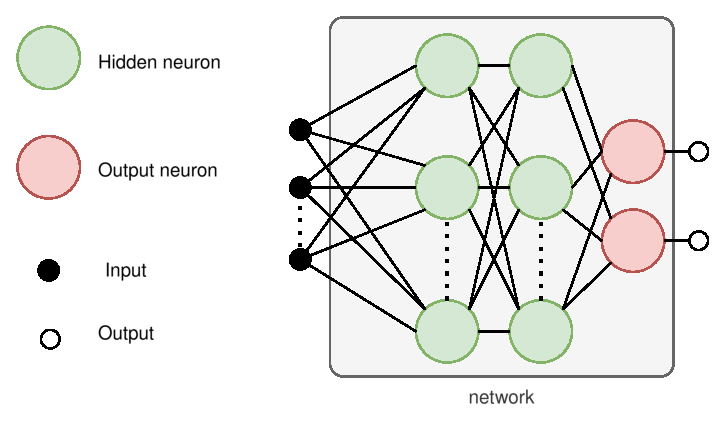
\includegraphics[]{figures/ann_model_configuration_mimo_with_legend.eps}
    {\footnotesize \textbf{(a)} \gls{mimoLabel} configuration\\}
    
    \vspace{1ex}
    
    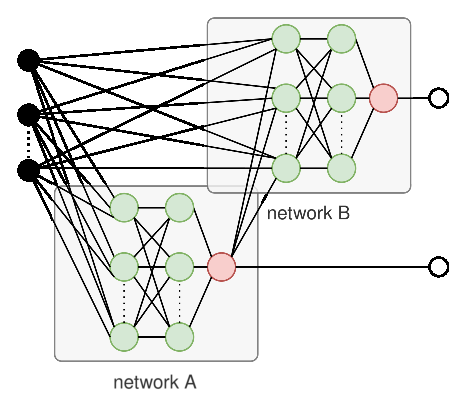
\includegraphics[]{figures/ann_model_configuration_cascade.eps}
    {\footnotesize \textbf{(b)} Cascade configuration}
    
    \caption{\acrshort{annLabel} model configurations}
    \labfig{intro:modelling:ann-model-configuration}
\end{marginfigure}

%As a result, this approach holds the promise of enhanced efficiency in model
%training, potentially requiring fewer data points for accurate predictions. 

% Tipos de red Feedforward Cascade-forward Radial-basis
\textbf{Network architectures}. Three network architectures have been
implemented and tested:
\begin{enumerate}
    \item \gls{ffLabel} network - \reffig{intro:modelling:ann-architectures}
    (a). This is the base network architecture, where different layers are
    added sequentially and the flow of information is unidirectional. The
    transfer function adopted in the hidden layers is the differentiable
    \textit{Log-Sigmoid}\sidenote{Defined as $logsig(x) = 1/(1 + e^{-x})$, mapping any real input to a value between 0 and
    1.}, whereas the one employed in the output layer is a linear one with no saturations.

    \item \gls{cfLabel} network - \reffig{intro:modelling:ann-architectures}
    (b). It is a variation on the feedforward network since it adds direct
    connections from the input and hidden layers to the output layer.

    \item \gls{rbfLabel} network - \reffig{intro:modelling:ann-architectures}
    (c). The transfer functions used in the first layer of the \gls{rbfLabel}
    network are different, they are local Gaussian like functions. Also,
    instead of multiplying by the weights, the distance between inputs and
    weights is computed and the bias is multiplied instead of added
    \sidecite{hagan_neural_2014}.
\end{enumerate}

% \begin{marginfigure}[]
%     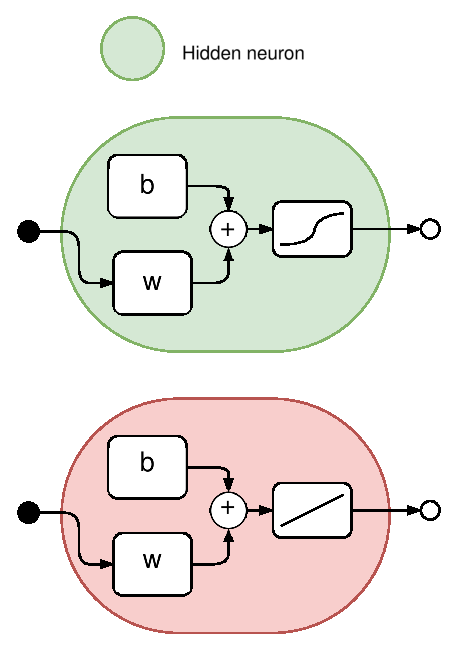
\includegraphics[]{figures/ann_neuron_type_simple_with_partial_legend.eps}
%     {\footnotesize \textbf{(a)} Feedforward\\} \vspace{2ex}
    
%     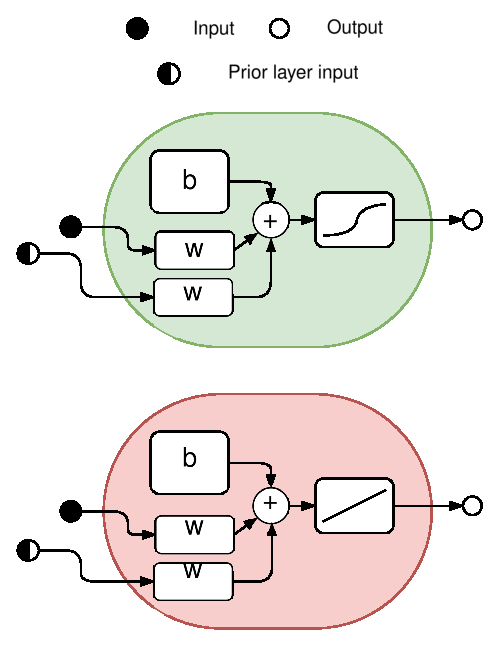
\includegraphics[]{figures/ann_neuron_type_cascade_with_partial_legend.eps}
%     {\footnotesize \textbf{(b)} Cascade-forward\\} \vspace{2ex}

%     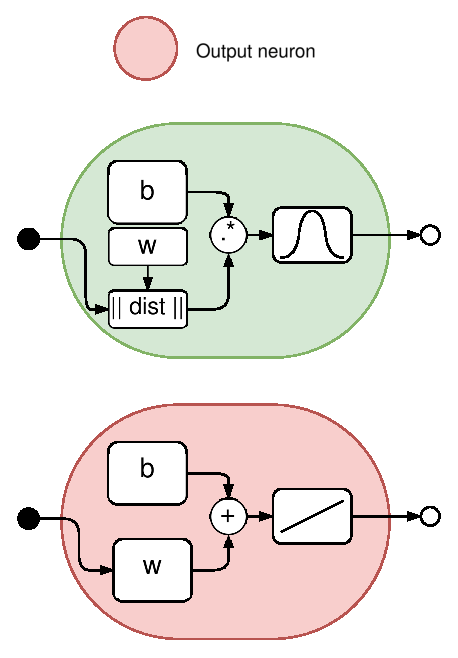
\includegraphics[]{figures/ann_neuron_type_radial_with_partial_legend.eps}
%     {\footnotesize \textbf{(c)} Radial-basis}

%     \caption{Considered \acrshort{annLabel} architectures}
%     \labfig{intro:modelling:ann-architectures}
% \end{marginfigure}

\begin{figure*}[h!]
    \centering
    \subfloat[\centering
    Feedforward]{{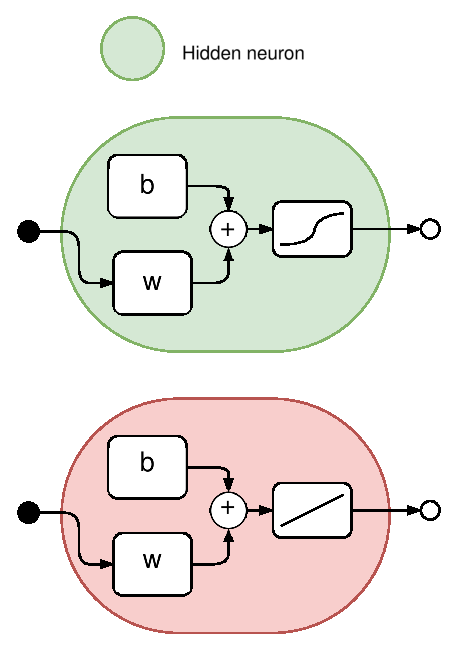
\includegraphics[width=0.32\textwidth]{figures/ann_neuron_type_simple_with_partial_legend.eps}
    }}%
    \qquad
    \subfloat[\centering
    Cascade-forward]{{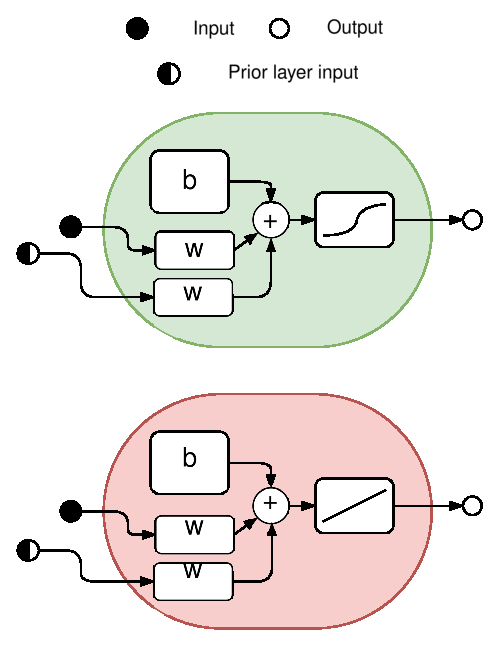
\includegraphics[width=0.32\textwidth]{figures/ann_neuron_type_cascade_with_partial_legend.eps}
    }}%
    \qquad
    \subfloat[\centering
    Radial-basis]{{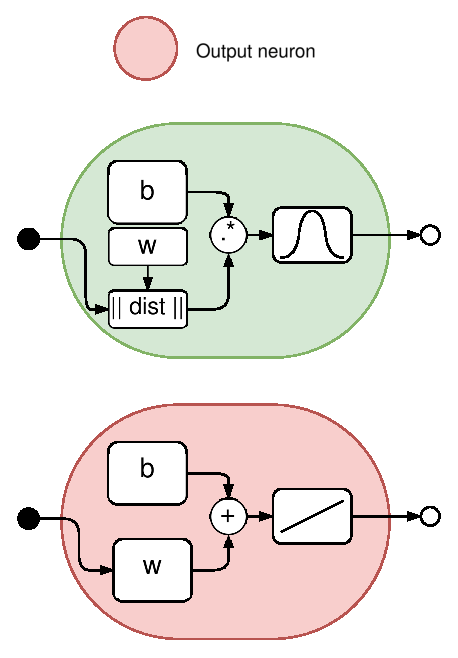
\includegraphics[width=0.32\textwidth]{figures/ann_neuron_type_radial_with_partial_legend.eps}
    }}%
    
    \caption{Considered \acrshort{annLabel} architectures}
    \labfig{intro:modelling:ann-architectures}
\end{figure*}

% topologías de red N de capas N de neuronas por capa

\textbf{Network topology}. Two-layer networks (one hidden and one output layer)
can learn almost any input-output relationship, including non-linear ones.
Adding more layers can improve the learning for more complex problems. However,
increasing the number of layers or neurons per layer increases the training
computational requirements, requires more data for a satisfactory model and can
lead to overfitting. Therefore, the process is usually started with two layers
and then the number of layers is increased if they do not perform
satisfactorily~\cite{hagan_neural_2014}. In this study, for the feedforward and
cascade-forward architectures, one and two hidden layers have been tested with
the following configurations: 5, 10, 20, 5-5, 5-10, 10-5, 10-10. For the case
of the \gls{rbfLabel}, it only has one hidden layer and neurons are added
sequentially during the training process up to a maximum which is set to 120
neurons.

% Procedimiento entrenamiento Justificar mejor elección de algoritmo de
% entrenamiento
\textbf{Training process}. The next important aspect to consider is the
training process. For the \gls{ffLabel} and \gls{cfLabel} networks many
Gradient- or Jacobian-based algorithms can be utilized. In this case, the
Levenberg-Marquardt backpropagation algorithm \sidecite{beale_neural_2010} has
been used. It is a fast algorithm, ideal for multilayer networks with up to a
few hundred weights and biases enabling efficient training. The training in
this case is done in batches since sequential training is slower and does not
produce better results. All data have been normalized applying the z-score
normalization method. 
% Early stop, paciencia For most applications of neural networks, the training
% error never converges to exactly zero. The error can reach zero for the
% perceptron network (radial basis network), but it is unlikely to happen for
% multilayer networks. For this reason, a criteria for deciding when to stop
% the training needs to be set in place, and this criteria needs provide a
% mechanism to avoid overfitting. 
The criteria established for deciding when to stop the training is the
following one:  when the performance on the validation set increases (worsens)
or when the  gradient is below a minimum ($1\times10^{-7}$) for a number of
iterations or epochs, or when a maximum number of 1000 epochs is reached. The
number of iterations to wait, often refereed as patience, is set to 6. Finally,
the selected network parameters will be those of the best epoch.

For each network architecture, the training process was repeated a total of ten
times (this is the recommended practice if the computational requirements allow
it, since it guarantees reaching a global optimum with a high degree of
confidence \sidecite{hamm_comparison_2007}). The optimal architecture and
training was selected according to a performance function, which in this case
has been the \gls{mseLabel} with the values normalized.

In the case of the \gls{rbfLabel} network, the chosen training method consists
in two stages which treats the two layers of the \gls{rbfLabel} network
separately. The first layer weights and biases are tuned based on the
orthogonal least squares method \sidecite{hagan_neural_2014}, while for the
second layer are computed in one step using a linear least-squares algorithm.
During training, neurons are added to the first layer (in increments of 20)
trying to minimize the \gls{mseLabel} to some goal, which in this case is set
depending on the case study: 10 for the \gls{mimoLabel} configuration and 0
($^\circ$C$^2$) and 20 (l$^2$/h$^2$) for temperature and water lost networks,
respectively, for the cascade configuration. Finally, a parameter called spread
is used to set the first layer biases. Larger values of this parameter promote
a smoother approximation of the training data (more generalization),
conversely, lower values provide a more exact fit to the training data. Values
from 0.1 to 30 have been tested for this parameter.


%================================
\subsubsection{Other machine learning methods}

\begin{itemize}
    \item \textbf{Random Forest}. A random forest for regression is a method
    that combines many decision trees to make more accurate and stable
    predictions. A decision tree is a model that splits the data into smaller
    and smaller groups based on input features, creating a set of simple rules
    that lead to a prediction at the end of each branch. Each tree in a random
    forest is trained on a slightly different version of the data by randomly
    sampling both data points and features, and the forest's final prediction is
    obtained by averaging the outputs of all trees. As the number of trees
    increases, the prediction error stabilizes and approaches a fixed value. The
    performance of a random forest depends on how strong the individual trees
    are at predicting the target and how different they are from each other, and
    this balance allows the method to produce reliable predictions that are
    usually better than those of a single decision tree~\sidecite{breiman_random_2001}. 
    
    \item \textbf{Gradient-boosting} builds a strong predictive model by
    combining many weak models, usually decision trees, in a sequential way. Each
    new tree is trained to correct the errors (residuals) made by the previous
    ensemble, using the gradient of a loss function to guide the
    improvements~\sidecite{friedman_greedy_2001}.
\end{itemize}


%===================================
%===================================
\subsubsection{Data-driven from first-principles models. Synthetic dataset generation}
\labsec{intro:modelling:sample-generation}

% Mencionar modelos basados en datos a partir de modelos físicos. Describir
% combinatoria sin detallar la combinatoria particular seguida para el modelo
% del CC.
One important advantage that first-principles models have over data-driven is
their scalability, that is, the ability to adapt a model developed and
validated in a pilot-scale system, to a large scale one. This is true for many
systems as long as the system configuration remains the same. This allows to
study and analyze pilot scale plants and extrapolate the results to industrial
sized plants. In addition, these type of model are also capable of predicting
the behaviour of the modelled systems in conditions that have not been tested
(\eg different operating or environmental conditions), although the
reliability of the model could be lower if these conditions move away from
those experimentally used for some parameter calibration.

On the contrary, data-driven models are very specific to the system and
operating ranges they are trained for. That is why training/calibrating a
data-driven model with data from a first-principles model is a common practice
to obtain a model that can be used in a larger range of operating conditions...

The process of generating samples from a first-principles model to train a
data-driven model is called sample generation. It consists of running the
first-principles model for a set of input parameters, which can be selected
randomly or following a specific distribution, and then using the outputs of
the first-principles model as the training data for the data-driven model.

The first step is to define the input parameters and their ranges. This can be
done by selecting the most relevant parameters for the system and determining
their ranges based on the system's operating conditions. The next step is to
generate a set of input parameters, which can be done using different methods
such as Latin Hypercube Sampling, Monte Carlo Sampling, Sobol Sampling, or
simply grid sampling. These methods allow to generate a set of input parameters
that cover the entire range of the input parameters and ensure that the
generated samples are representative of the system's behaviour. Once the input
parameters are defined, the first-principles model is run for each set of input
parameters, and the outputs of the model are recorded. Finally, the recorded
outputs are used to train the data-driven model.


%===================================
%===================================
\subsection{Discrete modelling by means of \glspl{fsmLabel}}
\labsec{intro:modelling:discrete}

So far we have discussed modelling of continuous systems, where changes evolve
smoothly over time, often described by differential equations. Discrete or
event-driven modelling, on the other hand, focuses on systems where the state
changes only at specific points in time in response to events.

There are many ways of modeling the behavior of these systems, and the use of
state machines is one of the oldest and best known. State machines allow us to
think about the ``state'' of a system at a particular point in time and
characterize the behavior of the system based on that state\sidenote[][*-3]{On each
different state, a process can be governed by different dynamics}.

For example, a traffic light can be described as a finite state machine with
three primary states: \textit{green}, \textit{yellow}, and \textit{red}. In each
state, the traffic light has a well-defined behavior (allowing vehicles to pass,
warning them to slow down, or stopping them completely). The transitions between
states are also clearly defined: green changes to yellow, yellow to red, and red
back to green. Some transitions are possible, while others are not (\eg, green
cannot jump directly to red without first passing through yellow).

\begin{marginfigure}[-3.5cm]
    \centering
    \includegraphics[width=.5\linewidth]{figures/fsm-traffic-light.png}
    \caption{\gls{fsmLabel} representation of a traffic light}
    \labfig{intro:modelling:fsm-traffic-light}
\end{marginfigure}


So, a state machine is a model of behavior composed of a finite number of
\textit{states} and \textit{transitions} between those states. Within each state and
transition some \textit{action} can be performed. A state machine needs to start at
some \textit{initial state}. Finite refers to a machine that has a limited number of
possible states and at any given time it will be in one of those states. Its
core components are described in the following:

\begin{itemize}
    \item \textbf{State}. A state represents a particular condition or stage in
    the state machine. It's a distinct mode of behavior or phase in a process.
    
    \item \textbf{Transition}. This is the process or event that causes the
    state machine to change from one state to another.

    \item \textbf{Action}. Specific operation or task that is performed when a
    certain event happens \ie a state is entered, exited, or during a
    transition.
    
    \item \textbf{Model}. A stateful structure that holds information about the
   state of the machine. It gets updated during transitions and defines
   actions.

    \item \textbf{Machine}. This is the entity that manages and controls the
    model, states, transitions, and actions. It's the conductor that
    orchestrates the entire process of the state machine.
\end{itemize}

\subsection{Forecasting and combinatory nature of \glspl{fsmLabel}}

A traffic light is a simple example of a deterministic state machine, because
its transitions are triggered by a single predictable input — the timer — and
therefore its future trajectory is entirely fixed. From any given state, there
is only one possible next step, so the entire cycle can be anticipated with
certainty (see \reffig{intro:modelling:fsms-evolution} (a)). Many real systems,
however, are not this simple. When the set of inputs that can trigger
transitions is larger and each input leads to different successor states, the
system no longer has just one linear trajectory but many possible ones. In such
cases, the behavior of the machine can be represented as a branching tree, where
each node corresponds to a state and each branch corresponds to a possible input
event. This can be illustrated for the traffic light example if a push-button is
added (see \reffig{intro:modelling:fsms-evolution} (b)). The state will be green
light unless the push-button is triggered. Starting from an initial state,
evaluating now the possible paths that yield in an arbitrary final state given a
number of steps becomes a combinatory problem. 

\begin{figure}
    \centering
    \subfloat[\centering Simple traffic light]{{\includegraphics[width=0.8\textwidth]{figures/fsm-evolution-simple-traffic-ligth.png}}}%
    \vspace{0.1cm}
    \subfloat[\centering Traffic light with push-button]{{\includegraphics[width=0.8\textwidth]{figures/fsm-evolution-traffic-ligth-with-pushbutton.png}}}%
    \caption[Evolution of different traffic-light \glspl{fsmLabel}]{Evolution of different traffic-light \glspl{fsmLabel} assuming the timer takes one step to complete.}
    \labfig{intro:modelling:fsms-evolution}
\end{figure}

This branching has important implications: while the machine is still finite in
the number of states, the number of possible sequences of states over the
horizon grows rapidly as more steps are considered. After just a few
transitions, the tree of possible futures can expand exponentially.

%===================================
%===================================
\subsection{Performance metrics}
\labsec{intro:modelling:metrics}

For models to be useful they need to accurately represent the real process. In
order to quantitatively assess how good a model represents a real system we use
different performance metrics. Four performance metrics are described hereinafter:
coefficient of determination (R$^2$), \gls[format=long]{rmseLabel},
\gls[format=long]{maeLabel} and \gls[format=long]{mapeLabel}. These metrics are
described below.

\textbf{Coefficient of determination}. Regression estimates the relationship
between input variables\sidenote{also known as features} and a continuous output
variable\sidenote{also refereed as target}. R$^2$ is a direct measure of
regression. It measures the proportion of the variance in the predicted variable
that can be attributed to the independent variable(s), in this case the
considered system inputs. Values close to one indicate a better prediction
accuracy. It is calculated as follows:

\begin{equation*}
    R^2 = 1 - \frac{\sum\limits_{i=1}^n (y_i - \hat{y}_i)^2}{\sum\limits_{i=1}^n (y_i - \bar{y})^2},
\end{equation*}

where $y_i$ is the measured or observed value for the output variable, in the
$i-th$ observation, $\hat{y}_i$ is the estimated value of the same variable and
$n$ is the total number of observations. Finally, $\bar{y}$ is the mean value
of the experimental values.


\textbf{Root Mean Square Error}. \gls{rmseLabel} is a statistical measure of
the difference between the values predicted by a model and the observed values.
It is calculated as the square root of the mean of the squared differences
between the predicted and observed values and it has its units. 

% \marginnote{
\begin{equation*}
    \mbox{RMSE} = \sqrt{\frac{1}{n} \sum\limits_{i=1}^n (y_i - \hat{y}_i)^2}
\end{equation*}
% }

\textbf{Mean Absolute Error}. It represents the average absolute difference
between predicted and actual values.

\begin{equation*}
    \mbox{MAE} = \frac{1}{n} \sum\limits_{i=1}^n \left|y_i - \hat{y}_i\right|
\end{equation*}

\textbf{Mean Absolute Percentage Error}. As the \gls{maeLabel}, it calculates
the difference between the predicted and the actual values, but in this case it
does so in relative terms:

\begin{equation*}
    \mbox{MAPE} = \frac{1}{n} \sum\limits_{i=1}^n \left| \frac{y_i - \hat{y}_i}{y_i} \right| \times 100\%
\end{equation*}


%================================
\subsection{Implementation software tools}
\labsec{intro:modelling:tools}

\begin{itemize}
    \item Gaussian Progress Regression de MATLAB~\sidecite{}
    \item Gaussian Progress Regression framework written in Python, from the Sheffield machine learning group~\sidecite{gpy2014}
    \item ANNs: ...~\sidecite{}
    \item Finite state machine modelling: transitions~\sidecite{}
\end{itemize}


%===================================
%===================================
%===================================
% \setchapterpreamble[u]{\margintoc}

% \chapter{Sensitivity analysis}
% \labch{intro:sa}

% It involves systematically assessing how variations in input parameters impact
% the model's outputs. In this case, the Sobol method
% \sidecite[3cm]{nossent_sobolsensitivity_2011}, which is a variance-based approach,
% has been used. This method decomposes the total variance of the model output
% into contributions from individual input parameters and their interactions. By
% quantifying the relative importance of each parameter, Sobol analysis
% facilitates the identification of influential factors, enabling a more nuanced
% understanding of complex systems characterized by numerous interacting
% variables.

% The analysis results are different sensitivities indices such as total sensitivity
% indices (total-order), first-order sensitivity indices (first-order), and
% interaction sensitivity indices (second-order). First-order measures the direct
% effect of an input variable on the output, excluding interaction effects with
% other variables, while the second-order measures specifically this interaction
% effects. Finally, total-order indices account for the total effect of an input
% variable, including both direct and interaction effects.


%===================================
%===================================
% \subsection{Sensitivity analysis as a model analysis tool}
% \labsec{intro:sa:modelling}

% Sobol sensitivity analysis provides a
% quantitative basis for assessing the consistency and validity of results when
% different approaches to model a system are compared. \glspl{annLabel} models
% with similar sensitivity analysis outcomes to those of the physical model,  are
% likely to capture the essential features of the system, offering a means to
% verify their credibility and ensuring that the proposed solutions align with
% the underlying physical principles. Therefore, Sobol sensitivity analysis
% emerges as a powerful tool not only for understanding the system input-outputs
% relationships, but also as a way to validate and compare various modelling
% approaches. The sensitivity analysis has been performed using \textit{SAlib},
% an open source sensitivity analysis tool for the \textit{Python} programming language
% \sidecite{herman_salib_2017,iwanaga_salib_2022}.


% %===================================
% %===================================
% \subsection{Sensitivity analysis as a measurement influence quantification tool}
% \labsec{intro:sa:measurement-influence}
% Sensitivity analysis can also be used to quantify the influence of measurement...

%TODO: Also check how it was defined in standardization article

%===================================
%===================================
% \setchapterpreamble[u]{\margintoc}
\section{Optimization}
\labsec{intro:optimization}

Optimization consists on finding the best solution, \ie the optimal solution, to
a problem under given circumstances. At its core, optimization seeks to
determine the values of decision variables that minimize (or maximize) an
objective function while respecting a set of constraints. These problems arise
in diverse domains such as operations research, economics, energy systems, and
machine learning, where they enable the systematic allocation of resources, the
design of efficient processes, and the balancing of trade-offs between competing
goals.

A general expression to define an optimization problem is:
\begin{equation}
    \min_{\mathbf{x},\, \mathbf{e};\, \boldsymbol{\theta}} \quad J = f(\mathbf{x}, \mathbf{e}; \boldsymbol{\theta}) 
    \quad \text{s.t.} \quad g_i(\mathbf{x}) \leq 0, \quad i = 1, \ldots, m
    \labeq{intro:optimization:general-expression}
\end{equation}

where $\mathbf{x}$ is the vector of decision variables, $f(\mathbf{x})$ is the
objective function to be minimized, and $g_i(\mathbf{x})$ are the constraints
of the problem. The objective function is a scalar function that maps the
decision variables to a real number, representing the cost or performance of the
system. The constraints are functions that restrict the feasible region of the
problem, defining the set of values that the decision variables can take. The
optimization problem is to find the values of the decision variables that minimize
the objective function while satisfying the constraints. 


\begin{marginfigure}[-3.5cm]
    \includegraphics[]{figures/contrained-optimization-vertical.jpg}
    \caption{Constrained optimization problem. The goal is to minimize $y=f(x)$
    with the two continuous  decision variables $x_1$ and $x_2$ constrained to
    $g(x)$. The problem is \gls{nlpLabel} with a convex solution-space.\\Source: Wang et
    al.~\cite{wang_structural_2020}}
    \labfig{intro:optimization}
\end{marginfigure}

Regarding the constraints, they can be categorized in two types depending
whether they can be evaluated before evaluating the objective function or not.:
\begin{itemize}
    \item \textbf{Bounds} or box-bounds. These are constraints that limit the range of the decision variables, such as
    \begin{equation*}
        x_i \in [l_i, u_i], \quad i = 1, \ldots, n
    \end{equation*}
    where $l_i$ and $u_i$ are the lower and upper bounds of the decision
    variable $x_i$, respectively.
    \item \textbf{Constraints}. These are constraints that restrict the
    feasible region of the problem, such as
    \begin{equation*}
        g_i(\mathbf{x}) \leq 0, \quad i = 1, \ldots, m
    \end{equation*}
    where $g_i(\mathbf{x})$ are the constraint functions that depend on the
    decision variables $\mathbf{x}$, and $m$ is the number of constraints. They
    can only be known after evaluating the objective function.
\end{itemize}


%===================================
%===================================
\subsection{\gls{nlpLabel} problems}
\labsec{intro:optimization:nlp_problems}

A \gls{nlpLabel} problem refers to a \emph{nonlinear programming} formulation in
which both the objective function $f(\mathbf{x})$ and the constraint functions
$g_i(\mathbf{x})$ can be nonlinear. These problems are generally more difficult
to solve than linear programming (LP) problems, since the feasible region may be
non-convex and the objective function may have multiple local minima. Solution
techniques for NLP include gradient-based methods, sequential quadratic
programming, interior-point methods, and heuristic approaches when derivatives
are unavailable or the problem is highly non-convex.

As an example, consider the following NLP problem:
\begin{equation}
    \begin{aligned}
        \min_{x_1, x_2} \quad & (x_1 - 2)^2 + (x_2 - 1)^2 \\
        \text{s.t.} \quad & x_1^2 + x_2^2 \leq 1, \\
                          & x_1, x_2 \in \mathbb{R}.
    \end{aligned}
    \labeq{intro:optimization:example_nlp}
\end{equation}
Here, the quadratic objective function is nonlinear as well as the circular constraint
$x_1^2 + x_2^2 \leq 1$. Both define convex regions so the problem is a convex \gls{nlpLabel}.

\begin{kaobox}[title=Optimization concepts]
    \begin{itemize}
        \item \textbf{Decision variables}. These are the variables that can be
        controlled or adjusted in order to optimize the objective function.
        
        \item \textbf{Objective function}. This is the function that needs to be
        minimized or maximized. It represents the goal of the optimization
        problem.

        \item \textbf{Constraints}. These are the restrictions or limitations
        that need to be satisfied in order to find a feasible solution. They can
        be equality or inequality constraints.

        \item \textbf{Search-space}. This is the set of all possible values
        of the decision variables that satisfy the bounds.

        \item \textbf{Feasible region}. This is the set of all possible values
        of the decision variables that satisfy the constraints. The optimal
        solution must lie within this region.

        \item \textbf{Optimal solution}. This is the set of values of the
        decision variables that minimize or maximize the objective function
        while satisfying all the constraints.

        \item \textbf{Convexity}. A problem is convex if both the objective
        function and the feasible region are convex. Convex problems have a
        single global optimum, which can be found efficiently using various
        optimization algorithms. Non-convex problems may have multiple local
        optima, making them more challenging to solve.
    \end{itemize}
\end{kaobox}

%===================================
%===================================
\subsection{\gls{minlpLabel} problems}
\labsec{intro:optimization:minlp_problems}

A \gls{minlpLabel} problem, or \emph{mixed-integer nonlinear programming},
extends the \gls{nlpLabel} formulation by introducing integer (often binary)
decision variables alongside continuous ones. The presence of discrete variables
significantly increases the complexity of the problem, as the feasible set
becomes combinatorial in nature, often leading to an exponential growth in the
search space. \gls{minlpLabel} problems naturally arise in many engineering
problems where decisions such as on/off states, integer quantities, or logical
relations must be combined with nonlinear models. Typical
solution strategies include branch-and-bound, branch-and-cut, outer
approximation, and decomposition methods.

As an example, consider the following \gls{minlpLabel} problem:
\begin{equation}
    \begin{aligned}
        \min_{x, y} \quad & (x - 3)^2 + y \\
        \text{s.t.} \quad & x^2 \leq y, \\
                          & x \in \mathbb{R}, \quad y \in \{0,1\}.
    \end{aligned}
    \labeq{intro:optimization:example_minlp}
\end{equation}
In this formulation, $x$ is a continuous variable, while $y$ is binary. The
feasible set is determined not only by the nonlinear constraint $x^2 \leq y$ but
also by the discrete choice of $y$, which switches the constraint on or off
depending on its value.

A common strategy for tackling \glspl{minlpLabel} is by integer
\emph{relaxation}, in which the integer constraints on some variables are
relaxed to continuous domains (e.g., replacing $y \in \{0,1\}$ with $y \in
[0,1]$). The relaxed problem becomes a standard \gls{nlpLabel}, which is
typically easier to solve. The solution of this relaxation can then be used to
guide exact methods such as branch-and-bound or to construct valid lower bounds
in global optimization algorithms. However, this is flawed in assuming the best
solution of the relaxed problem is close to the full \gls{minlpLabel}
problem solution, or that the relaxed problem contains relevant information in
its gradient.

\subsection{A discussion on constraint handling}
\labsec{intro:optimization:constraints}

There are two main approaches to handle constraints in optimization problems:
\begin{itemize}
    \item \textbf{Penalty methods}. These methods add a penalty term to the
    objective function to penalize the violation of the constraints. The
    penalty term is usually a function of the constraint violation, and it is
    added to the objective function to form a new objective function that is
    minimized. The penalty term can be linear or non-linear, and it can be
    adjusted during the optimization process to ensure that the constraints are
    satisfied. The main advantage of penalty methods is that they allow to
    handle constraints in a flexible way, and they can be used with any
    optimization algorithm. However, they can also lead to suboptimal solutions
    if the penalty term is not properly tuned, and they can also lead to
    numerical instability if the penalty term is too large.
    
    \item \textbf{Constraint handling methods}. These methods handle the
    constraints directly, by either rejecting solutions that violate the
    constraints or by modifying the optimization algorithm to ensure that the
    constraints are satisfied. The main advantage of constraint handling
    methods is that they guarantee that the constraints are satisfied, and they
    can also lead to better solutions than penalty methods. However, they can
    also be more complex to implement, and they can also lead to numerical
    instability if the constraints are too restrictive. Specific
    constraint-handling capable algorithms are required to solve these type of
    problems.
\end{itemize}

By using inequality constraints, the optimization algorithm is forced to find
the \textit{best} solution that satisfies the constraints, however, in a
problem with a horizon window, this would require returning a value of the
constraint for each step in the horizon window. Thus, producing a large vector
of inequality constraints and increasing the dimension of the problem (\ie its
complexity). On the other hand returning a single value for the whole episode
gives little information to the algorithm on how to adapt its decision values
to satisfy the constraint and thus might be unable\sidenote{By unable we are
referring to requiring an unfeasible amount of objective function evaluations,
too much time.} to converge to a solution.

Finally, non constraint-handling capable algorithms can be wrapped with
constraint handling methods to solve problems with
constraints~\sidecite{farmani_selfadaptive_2003}, where they basically
implement some type of penalty method.

%===================================
%===================================
\subsection{Multi-objective optimization}
\labsec{intro:optimization:multi-objective}

When an optimization problem involves only one objective function, the task is
called single-objective optimization. In contrast, when multiple objectives
must be optimized simultaneously, the problem becomes one of multi-objective
optimization. A key difference is that in the multi-objective case, objectives
are often conflicting: improving one objective typically requires sacrificing
performance in another~\sidecite{deb_multiobjective_2011}. As Johan Löfberg illustrates
in the \href{https://yalmip.github.io/multi-objective-problems}{YALMIP
documentation}:

\begin{quote}
    It is impossible to design a car which is as light as possible, as cheap as
    possible, as fast as possible, and as durable as possible, all at the same
    time. In the end, the solution to the obviously multi-objective task of
    designing a car, will be a compromise. Multi-objective optimization is about
    finding the set of non-bad compromises, which is called the Pareto-optimal
    solutions.
\end{quote}

Two main approaches are commonly used to address multi-objective problems~\cite{deb_multiobjective_2011}:
\begin{itemize}
    \item Scalarization (or decomposition) methods, where the multi-objective
    problem is converted into a sequence of single-objective problems by
    combining objectives into one, for example using weighted sums or penalty
    methods. Each run of a single-objective solver yields one trade-off
    solution, so multiple runs with different scalarizations are required to
    approximate the Pareto set.
    \item Population-based methods, such as evolutionary
    algorithms\sidenote{Described in the following}, which evolve a set of
    solutions in parallel. Because they operate on a population rather than a
    single solution, these methods naturally approximate the entire Pareto front
    within a single run, capturing multiple trade-offs between conflicting
    objectives.
\end{itemize}


%===================================
%===================================
\subsection{Optimization algorithms}
\labsec{intro:optimization:algorithms}

Optimization algorithms are methods designed to find the best solution to a
problem by minimizing or maximizing an objective function under given
constraints. Two categories are distinguished: local and global. 

\subsubsection{Local optimization}

For convex problems and gradient-based methods, they typically use derivative
information to guide the search efficiently.

\begin{itemize}
    \item \textbf{Interior Point OPTimizer
    (IPOPT)}~\sidecite{wachter_implementation_2006} is a numerical optimization
    algorithm for large-scale nonlinear programming (NLP) problems. It uses a
    primal-dual interior-point method, solving a sequence of barrier subproblems
    to handle inequality constraints while maintaining feasibility. At each
    iteration, IPOPT computes a Newton-type step by solving the sparse
    Karush-Kuhn-Tucker system, simultaneously updating primal and dual
    variables. Line search and barrier parameter updates ensure convergence,
    even for non-convex problems. Its highly efficient with sparse derivative
    matrices.
    
    \item \textbf{Compass search}~\sidecite{kolda_optimization_2003} is a
    derivative-free local optimization method belonging to the class of direct
    search algorithms. At each iteration, the algorithm evaluates the objective
    function by probing in coordinate directions (north, south, east, west in
    two dimensions, or along each axis in higher dimensions) from the current
    point. If a trial move in any direction improves the objective, the
    algorithm accepts the move and continues from the new point; otherwise, the
    step size is reduced, and the process repeats. It is a slow but sure local
    optimization algorithm.
\end{itemize}


\subsubsection{Gradient-free global optimization}

\epigraph{Global optimization: The holy grail! 60\% of the time it works every time.}{\small Johan Löfberg \\ Creator of YALMIP}

Global gradient-free optimization refers to a family of optimization methods
that aim to find the best solution to a problem without relying on gradient
information. These methods are especially useful when the objective function is
non-differentiable, noisy, discontinuous, or available only through expensive
simulations where derivatives are impossible or impractical to compute. Unlike
local optimization methods that may get trapped in nearby minima, global
approaches search the entire solution space to increase the chances of finding
the true global optimum.

\glspl[format=long]{gaLabel} and \glspl[format=long]{esLabel} are both part of
the evolutionary computation family\sidenote{they try to optimize a problem by
iteratively trying to improve a candidate solution with regard to a given
measure of quality}, but they emphasize different mechanisms. \glspl{gaLabel},
introduced by Holland~\sidecite{holland_adaptation_1992}, are inspired by
biological evolution and work mainly with populations of candidate solutions
represented as strings, often binary. They rely heavily on crossover
(recombining parts of two solutions) along with mutation and selection, and are
frequently applied to discrete or combinatorial problems. In contrast, \gls{esLabel},
pioneered by P. Bienert, I. Rechenberg, and H. Schwefel in the
60s~\sidecite{rechenberg_evolution_1989,schwefel_numerical_1981}, were designed
for continuous optimization tasks and emphasize mutation as the primary search
operator. A defining feature of \gls{esLabel} is self-adaptation: not only the solutions
but also the mutation parameters (such as step sizes or covariance structures)
evolve over time, allowing the algorithm to adjust its own search
dynamics\sidenote{Crossover does exist in \gls{esLabel} but plays a secondary role
compared to \glspl{gaLabel}}.

\begin{kaobox}[title=Genetic Algorithms versus Evolutionary Strategies]
    An interesting reflection from Francesco Biscani and Dario Izzo~\cite{biscani_parallel_2020}:
    Approximately during the same decades as Evolutionary Strategies were
    studied, a different group led by John Holland, and later by his student
    David Goldberg, introduced and studied an algorithmic framework called
    “genetic algorithms” that were, essentially, leveraging on the same idea but
    introducing also crossover as a genetic operator. This led to a few decades
    of confusion and discussions on what was an evolutionary strategy and what a
    genetic algorithm and on whether the crossover was a useful operator or
    mutation only algorithms were to be preferred.
\end{kaobox}

\begin{kaobox}[title=Local versus gradient-free global optimization]
    When suitable, local optimization algorithms are generally preferable to
    heuristic approaches, as they typically achieve higher precision with far fewer
    function evaluations and offer more reliable convergence properties. Heuristic
    methods, in contrast, often demand significantly larger computational effort and
    may still fail to reach the desired solution quality. Their use should therefore
    be limited to situations where gradient information is unavailable or the
    problem structure prevents the application of more efficient local
    techniques. \\

    Some of the algorithms presented here can theoretically, for any given finite
    problem, terminate with a global optimal solution as their parameters enable for
    a more extensive search. This theoretical result, however, is not particularly
    helpful, since the time required to ensure a significant probability of success
    will usually exceed the time required for a complete search of the solution
    space. \\

    The objective is to the best alternative for a particular problem that can
    consistently find good solutions given some computational budget.    
\end{kaobox}

The following global optimization algorithms have been used in this research
work:\todo{Añadir figuras para visualizar algunos de los algoritmos}

\begin{marginfigure}[-8.5cm]
    \includegraphics[]{figures/simmulated_annealing.png}
    \caption{Simulated Annealing. Example illustrating the effect of cooling
    schedule on the performance of simulated annealing. The problem is to
    rearrange the pixels of an image so as to minimize a certain potential
    energy function, which causes similar colors to attract at short range and
    repel at a slightly larger distance. The elementary moves swap two adjacent
    pixels. These images were obtained with a fast cooling schedule (left) and a
    slow cooling schedule (right), producing results similar to amorphous and
    crystalline solids, respectively. \\
    Source: \href{https://en.wikipedia.org/wiki/Simulated_annealing}{Wikipedia}}
    \labfig{intro:optimization:sa}
\end{marginfigure}

\begin{itemize} 
    \item \textbf{(N+1)-ES Simple Evolutionary Algorithm (SEA)}~
    \sidecite{rechenberg_evolution_1989,schwefel_numerical_1981,biscani_parallel_2020}.
    Basic evolutionary strategy algorithm, where a population of individuals at
    each generation produces one offspring by mutating its best individual
    uniformly at random within the bounds. Should the offspring be better than
    the worst individual in the population it will substitute it.

    \item \textbf{Simple Genetic Algorithm
    (SGA)}~\sidecite{holland_adaptation_1992},~\cite{biscani_parallel_2020}.
    Basic genetic algorithm where a population of individuals evolves through
    selection, crossover, and mutation. New offspring are generated by combining
    the genetic material of selected parents, and the population is updated by
    replacing less fit individuals with the newly created ones.

    \item \textbf{Covariance Matrix Adaptation Evolution Strategy
    (CMA-ES)}~\sidecite{hansen_cma_2006,gendreau_handbook_2010},~\cite{biscani_parallel_2020}
    iteratively samples candidate solutions from a multivariate normal
    distribution whose parameters are adapted over time. The distribution mean
    is updated toward successful candidate solutions, while the covariance
    matrix is incrementally adjusted to increase the likelihood of previously
    successful search directions, a process that can be interpreted as a natural
    gradient descent and as an iterated principal component analysis of
    successful steps. In addition, CMA-ES maintains two evolution paths that
    track the correlation between consecutive steps: one path accelerates the
    adaptation of the covariance matrix by reinforcing favorable directions,
    while the other provides a robust mechanism for step-size control. This
    dynamic adaptation of both the covariance structure and step size allows
    CMA-ES to balance exploration and exploitation effectively, prevent
    premature convergence, and achieve fast progress toward optima even in
    high-dimensional, ill-conditioned, or nonconvex landscapes.

    \item \textbf{Extended Ant Colony Optimization
    (GACO)}~\sidecite{schluter_extended_2009},~\cite{ biscani_parallel_2020}.
    Ant Colony Optimization (ACO) is a class of optimization algorithms inspired
    by the foraging behavior of ants. Artificial `ants' explore a parameter
    space representing all possible solutions, recording their positions and
    solution quality. Similar to real ants laying pheromones to guide others,
    simulated ants use this information so that future iterations increasingly
    focus on better solutions. An extended version called Extended
    ACO~\cite{schluter_extended_2009} generates new solutions using a
    multi-kernel Gaussian distribution based on pheromone-like values derived
    from previous solution quality. Solutions are ranked using an oracle penalty
    method. Extended ACO can handle box-bounded single-objective problems, both
    constrained and unconstrained, with continuous or integer variables.
    
    \item \textbf{Particle Swarm Optimization}
    (PSO)~\sidecite{kennedy_particle_1995,
    gad_particle_2022},~\cite{biscani_parallel_2020} is a population-based,
    derivative-free optimization algorithm inspired by the collective behavior
    of bird flocks. Each particle represents a candidate solution and moves
    through the search space with a velocity influenced by its personal best
    position and the global or neighborhood best positions. Through iterative
    updates of positions and velocities, the swarm balances exploration and
    exploitation to converge toward optimal solutions.
    
    \item \textbf{Self-adaptive Differential Evolution}
    (SADE)~\sidecite{storn_differential_1997, brest_selfadapting_2006,
    elsayed_differential_2011},~\cite{biscani_parallel_2020}. In the original
    differential evolution algorithm~\cite{storn_differential_1997}, at each
    iteration, new candidate solutions are generated by combining the weighted
    difference of randomly selected individuals with another individual from the
    population. This mutation step is followed by crossover to increase
    diversity, and selection ensures that only the better solutions survive.
    Many different proposals have been made to self-adapt both the crossover
    probability and the differential weight parameters of the original
    differential evolution algorithm. The used optimization library
    ~\cite{biscani_parallel_2020} implements two different mechanisms-Brest et
    al. ~\cite{brest_selfadapting_2006} and Elsayed et
    al.~\cite{elsayed_differential_2011} - together with their own addition.
    
    \item \textbf{Simulated annealing - Corana's version}
    (SA)~\sidecite{corana_minimizing_1987},~\cite{gendreau_handbook_2010,
    biscani_parallel_2020} is a stochastic, derivative-free optimization
    algorithm inspired by the annealing process in metallurgy. The defining
    feature of simulated annealing is its use of a temperature parameter that
    decreases gradually during the search. The algorithm begins with a high
    initial temperature, allowing it to explore the search space freely and
    accept worse solutions with higher probability. As the temperature is
    reduced according to an annealing schedule specified by the user, the
    algorithm increasingly focuses on low-energy (or low-cost) regions and
    eventually behaves like a steepest descent method. This cooling process
    helps the system move from broad exploration toward fine-grained
    exploitation. Corana's version of SA introduces coordinate-wise temperature
    adaptation, where each variable has its own temperature schedule, and the
    step size is adjusted based on the success rate of previous moves. This
    allows the algorithm to adaptively balance exploration and exploitation for
    each dimension, improving convergence on high-dimensional or rugged
    landscapes.
    
    \item \textbf{(Improved) Harmony Search}
    (IHS)~\sidecite{geem_new_2001},~\cite{biscani_parallel_2020} inspired by the
    improvisation process of musicians, each musician represents a decision
    variable where each note corresponds to a value, and the aim is to achieve
    the best possible harmony—analogous to finding the global optimum.  In
    practice, every member of the population contributes to the search. At each
    iteration, a new solution is generated and, if it performs better than the
    worst individual in the population, it replaces it. The number of fitness
    function evaluations is therefore equal to the number of iterations. An
    improved version in Biscani et al.~\cite{biscani_parallel_2020} of HS
    introduces dynamic parameters: the probability of reusing values from the
    decision vector is adjusted linearly, while the mutation rate decreases
    exponentially over time. These refinements are designed to balance
    exploration and exploitation more effectively\sidenote[][*-2]{While HS has
    demonstrated competitive results, it has also been criticized for its
    metaphor: the musical analogy adds little explanatory value and may obscure
    the algorithm's mechanics, which in essence resemble those of
    \glspl{esLabel} or \glspl{gaLabel}, relying on concepts such as mutation and
    crossover.}
\end{itemize}

\begin{marginfigure}[-8.5cm]
    \includegraphics[]{figures/particle-swarm-optimization.png}
    \caption{Particle Swarm Optimization concept. Each particle adjusts its
    velocity based on its own experience and that of neighboring particles to
    explore the search space and converge towards optimal solutions.\\Source:
    \href{https://esa.github.io/pagmo2/docs/cpp/algorithms/pso.html}{Pagmo
    2.19.1 documentation}}
    \labfig{intro:optimization:pso}
\end{marginfigure}


\begin{figure*}
    \centering
    \subfloat[\centering CMA-ES \\ Source: \href{https://en.wikipedia.org/wiki/File:Concept_of_directional_optimization_in_CMA-ES_algorithm.png}{Wikipedia}]{{\includegraphics[width=0.48\linewidth]{figures/Concept_of_directional_optimization_in_CMA-ES_algorithm.png}}}%
    \hspace{0.01\linewidth}
    \subfloat[\centering Compass-search \\ Source: \href{https://esa.github.io/pagmo2/docs/cpp/algorithms/compass_search.html}{Pagmo 2.19.1 documentation}]{{\includegraphics[width=0.44\linewidth]{figures/compass-search.png}}}%
    \caption[Illustration of optimization runs for two algorithms]{Illustration of optimization runs for two algorithms. In CMA-ES (a) it shows the covariance matrix adaptation on a simple two-dimensional problem. The spherical optimization landscape is depicted with solid lines of equal f-values. It  shows how the distribution (dotted line) of the population (dots) changes during the optimization. On this simple problem, the population concentrates over the global optimum within a few generations.}
    \labfig{label:context:descriptor}
\end{figure*}



In this research work the two problems that are going to be presented on each
part are non linear and non-convex. One of them also includes constraints.
Meta-algorithms enable adapting algorithms that would otherwise be limited for
some types of problem to be used by wrapping the optimization algorithm with the
so-called meta-algorithm, two are used:

\begin{itemize}
    \item \textbf{Monotonic Basin Hopping} (MBH)~\cite{biscani_parallel_2020} is
    an optimization algorithm that combines local search with stochastic
    exploration. It repeatedly perturbs candidate solutions within a neighborhood
    and applies a local optimization algorithm to find nearby minima. If the best
    solution improves, it is updated; otherwise, the search resets. This iterative
    approach allows the algorithm to escape local minima and efficiently explore the
    landscape in search of the global optimum.
    
    \item \textbf{Self-adaptive fitness formulation for constrained
    optimization} (CSTR-SA)~\sidecite{farmani_selfadaptive_2003}. The
    self-adaptive constraint-handling meta-algorithm allows any single-objective
    unconstrained algorithm to solve constrained problems. It adapts its
    parameters based on the current population, using a penalty approach that
    accounts for constraint violations. Each individual is evaluated by both
    objective value and normalized constraint infeasibility, and the population
    is evolved using the wrapped algorithm with penalized objectives. The best
    individuals are reinserted immediately, influencing the next generation,
    making this approach compatible with non-generational evolutionary
    algorithms.
\end{itemize}


%================================
\subsection{Implementation software tools}
\labsec{intro:modelling:tools}

\begin{itemize}
    \item PyGMO~\sidecite{biscani_esa_2021} is a scientific Python library for massively parallel optimization. It is built around the idea of providing a unified interface to optimization algorithms and to optimization problems and to make their deployment in massively parallel environments easy.
\end{itemize}


%===================================
%===================================
% \setchapterpreamble[u]{\margintoc}
\section{Control}
\labsec{intro:control}

Controllers are mechanisms that allow us to manipulate the behavior of a
system. While modeling and simulation provide a way to passively describe and
predict how a system evolves, controllers take the next step by actively
influencing the system in order to promote a desired behavior. In this way,
controllers are fundamental to turning a passive system description into an
autonomous system capable of regulating itself and achieving specific goals.

\begin{figure*}
    \centering
    \subfloat[\centering Open-loop]{{\includegraphics[width=0.52\linewidth]{figures/control-open-loop.png}}}%
    \hspace{0.01\linewidth}
    \subfloat[\centering Closed-loop]{{\includegraphics[width=0.44\linewidth]{figures/control-closed-loop.png}}}%
    \caption{Control diagrams}
    \labfig{intro:control-diagrams}
\end{figure*}

The general workflow of control engineering is: start with a dynamical system
of interest, develop a mathematical model that captures its essential
behavior, and then design a control policy that drives the system toward the
desired performance. Depending on how this is achieved, different types of
control strategies can be distinguished:

\begin{itemize}
    \item Passive control: The desired behavior is embedded into the design of
    the system itself, without requiring active intervention. For example,
    designing a building with proper thermal insulation ensures it maintains
    stable indoor temperatures without external control actions.
    
    \item Active control: The controller actively supplies energy or signals to
    the system in order to adjust its behavior. Active control can be further
    classified into:
    \begin{itemize}
        \item Open-loop control: A sequence of control actions (or a predefined
        trajectory) is computed in advance and applied to the system without
        measuring its actual response. This approach is simple but fragile,
        since it assumes the system will behave exactly as predicted.
        \item \textbf{Closed-loop (feedback) control}: The controller continuously
        measures the outputs of the system and adjusts its actions based on the
        observed behavior. This feedback mechanism allows the system to
        autonomously correct deviations and respond to changes in real time.
    \end{itemize}
\end{itemize}

Feedback control, in particular, offers several fundamental advantages over open-loop strategies:

\begin{itemize}
    \item Robustness to uncertainty: Real systems are never perfectly
    known—models are approximations, and parameters may vary. Feedback allows
    the controller to adapt its actions on the fly, reducing the impact of
    modeling errors.
    \item Rejection of disturbances: External disturbances, whether measurable
    or not, can affect the system output. Feedback enables the controller to
    partially or fully counteract these disturbances.
    \item Stability enhancement: A system that is unstable when uncontrolled
    (open-loop) can often be stabilized through properly designed feedback,
    ensuring safe and predictable behavior.
\end{itemize}

Summarizing, control theory provides a framework that transforms dynamical
systems from passive entities into actively regulated, autonomous ones. Through
feedback, controllers achieve robustness, disturbance rejection, and stability.

\begin{kaobox}[title=A practical example: a washing machine]
    In a washing machine our objective is to have clean clothes after the
    washing is done, this would be the desired output. The control actions are
    mainly water, soup and temperature. The open-loop control of a washing
    machine consists on a predefined set of programs. Once the operator chooses
    one program, the washing machine control system will go through the cycle
    regardless of the load: how many clothes were added, how dirty they are, how
    powerful the soap used is, etc. \\
    
    While this is often enough there is a risk
    of overusing resources (cleaning too much) or failing to properly clean
    them. A washing machine that could measure for example how dirty the outlet
    water is (\ie having cleanliness feedback), it could continue cleaning just
    enough until a satisfactory cleanliness level, potentially using fewer total
    resources (more efficient use of water and soup) or it would continue
    cleaning for longer if specially dirty clothes were to be clean, reaching
    the desired \textit{clean clothes} output. 
\end{kaobox}
 

%===================================
%===================================
\subsection{PID controllers}
\labsec{intro:control:pid}

A \gls{pidLabel} controller is one of the most widely used feedback control
strategies in engineering~\sidenote{Honorable mention here to \gls{mpcLabel}
control, not used in this research work but widely used in the industry for
complex and effective process control, it shares many similarities to the
optimization just described above and the reader is referred to Camacho et
al.~\cite{camacho_model_2007}} because it combines three complementary
mechanisms that work together to regulate a system
effectively~\sidecite{hagglund_advanced_2006}. The proportional term (P)
generates a control action directly proportional to the instantaneous error
e(t), which is the difference between the desired setpoint and the actual
process variable; this provides an immediate response that reduces deviations.
However, proportional action alone often leaves a steady-state error, which is
corrected by the integral term (I). By integrating the error over time, the
integral term accumulates past deviations and adjusts the control signal until
the steady-state error is eliminated, ensuring that the system output eventually
matches the setpoint exactly. While proportional and integral actions ensure
responsiveness and accuracy, they may lead to sluggishness or overshoot if the
system changes rapidly. To address this, the derivative term (D) predicts future
behavior by considering the rate of change of the error, effectively damping
oscillations and improving stability by anticipating trends before they cause
large deviations. Together, these three terms balance immediate reaction,
long-term correction, and predictive adjustment, resulting in the general
\gls{pidLabel} control law:

\begin{equation}
u(t) = K \left( e(t) + \frac{1}{T_i} \int_{0}^{t} e(\tau)\, d\tau + T_d \frac{de(t)}{dt} \right).
\end{equation}

where K is the proportional gain, Ti the integral time, and Td​ the derivative
time. By tuning these parameters appropriately, the \gls{pidLabel} controller can be
adapted to a wide variety of dynamic systems, offering both robustness and
simplicity, which explains its success and popularity in industrial and
scientific applications. PI controllers, are sufficient for many control
problems, particularly when process dynamics are benign and the performance
requirements are modest. This is the case in the processes of this research
work, however, some enhancements\sidenote{This is not an extensive list,
there are many others advanced extensions that can be applied to the
architecture, tuning of the controller, process identification, dead-time
compensators, etc. that are out of the scope of this research work. \\The reader
is referred to Hägglund and Åström~\cite{hagglundtore_advanced_2006} and Normey-Rico~\cite{normey-rico_control_2007}} can be
applied to extend the basic \gls{pidLabel} scheme:

\begin{itemize}
    \item Anti-windup on the integral action\todo{}
    \item Feedforward\todo{}
\end{itemize}


%================================
\subsection{Implementation software tools}
\labsec{intro:modelling:tools}

\begin{itemize}
    \item simple-pid
\end{itemize}


%===================================
%===================================
\section[Hierarchical control]{Hierarchical control: how optimization and control come together}[Hierarchical control]
\labsec{intro:hierarchical-control}

Ideally, a centralized solution would handle both low-level process control
tasks and higher-level resource management and distribution optimization.
However, this is rarely the case. For instance, planning the optimal
distribution of resources on a monthly basis may require solving a complex
optimization problem, often with a combinatorial component. Such optimization is
computationally expensive, so it is typically addressed using simplified process
models with long sampling periods, and the computation of new decisions is
performed only occasionally.

In contrast, low-level process control requires frequent updates of control
actions that must be computed quickly. A single centralized system attempting to
address both high- and low-level problems would therefore face major challenges.
Moreover, in large-scale systems, any failure of this centralized solution could
compromise many—often critical—processes. For these reasons, decentralized and
distributed approaches are often preferred.

In such approaches, complexity is divided among different agents (or layers).
Each agent has a limited, problem-specific set of responsibilities. Various
architectures exist for managing the information exchange between these agents.
Summarizing, the factors that justify the need of a decentralized solution
are~\sidecite{scattolini_architectures_2009}:

\begin{itemize}
    \item Different time scales between low- (in the order of seconds) and
    high-level (in the order of hours) layers
    \item Different dynamic behavior: usually fast for regulatory control, slow
    or static for upper layers.
    \item Different computing requirements: complex resource optimization
    compared to generally more straightforward process control\sidenote{depends
    on the particular problem, they can get very complex too}
    \item Decoupling between optimization and critical process control
\end{itemize}

In this research, a hierarchical two-layer control architecture is adopted as
visualized in \reffig{intro:hierarchical-control}. At the upper layer, a \gls{rtoLabel} determines the
optimal operating conditions with respect to an economic performance index,
using a detailed but static nonlinear physical model of the system. The lower
layer relies on a simpler linear dynamic model—often derived through
identification experiments—to design regulators such as \gls{mpcLabel} or
\gls{pidLabel} controllers that ensure the \gls{rtoLabel} targets are met, while
also providing bottom-up feedback on constraints and performance. Despite its
static nature, the \gls{rtoLabel} model should be periodically updated through
reconciliation procedures to adapt to slow disturbances, consistency must be
maintained between the models used at the upper and lower layers, and
steady-state optimization must guarantee that the computed input and output
references are both feasible and as close as possible to the desired
setpoints~\cite{scattolini_architectures_2009}.

\begin{marginfigure}[-5.5cm]
    \includegraphics[]{figures/hierarchical-architecture-diagram.png}
    \caption{Hierarchical control architecture}
    \labfig{intro:hierarchical-control}
\end{marginfigure}

%================================
\subsection{Implementation software tools}
\labsec{intro:hierarchical:tools}

\begin{itemize}
    \item Airflow during the implementation. For the management and launching of
    the upper layer optimization scripts.
\end{itemize}

%----------------------------------------------------------------------------------------
%	SOLARMED
%----------------------------------------------------------------------------------------
% \pagelayout{wide} % No margins
\addpart{Energy management in MED processes driven by variable energy sources}
\pagelayout{margin} % Restore margins

\tldrbox{
    ...
}

% Visual abstract
a\todo{Add visual abstract}

\section*{Derived scientific contributions}
\addcontentsline{toc}{section}{Derived scientific contributions}

\section*{Structure}
% %===================================
%===================================
%===================================
\setchapterpreamble[u]{\margintoc}
\chapter{(Pendiente mover) SolarMED pilot plant description}
\labch{solarmed:pilot-plant}

The \gls{solarmedLabel} system is an \gls{medLabel} plant that receives its
thermal energy from a solar field + thermal storage system as depicted in
\reffig{solarmed:pilot-plant:diagram}: a flat plate
collector solar field which is the heat source, a pressurized hot water
two-tank thermal storage system, and an \gls{medLabel} plant which uses this
heat to separate seawater into fresh water and brine. The solar field and
thermal storage circuits are separated by a heat exchanger.

% TODO: A esta figura quitar colores de decision variable and environment
% variables, solo color neutro
\begin{figure*}[h!]
	\includegraphics[]{figures/SolarMED-process-diagram.png}
	\caption{\gls{solarmedLabel} process diagram}
	\labfig{solarmed:pilot-plant:diagram}
\end{figure*}

% \setchapterpreamble[u]{\margintoc}
\chapter{Performance evaluation in MED processes: standard methodology proposal}
\labch{solarmed:std}

\tldrbox{
    This chapter presents a standard method for performance evaluation of MED
    processes, which can also be extrapolated to other thermal separation
    processes. This method considers crucial aspects such as instrumentation
    requirements, process control, and the adequacy of performance metrics,
    including uncertainty in their determination. In addition, we have
    developed an algorithm for the automatic identification of steady-state
    operation, which allows to increase the reliability and robustness of
    evaluations under such variable conditions. The experimental results also
    show that the proposed method is robust and reliable, allowing for a fair
    comparison of MED processes under different conditions.

    The experimentation includes the evaluation of the process at high TBTs.
    The results are analyzed using different performance metrics and the scale
    formation risk is estimated by the \fullgls{rsiLabel}. The results show
    that the MED process can be operated at high TBTs without significant scale
    formation, but also without significant improvements in thermal performance
    or reconcentration capacity if no changes to its design are made. 
}

\section*{Introduction}
% Estado del arte
The only standard existing in MED is not related to performance evaluation, but to cost structures and determinants \cite{pinto_desalination_2017}. For the performance evaluation of MED processes, originally, the index Gain Output Ratio ($GOR$) was used for plants operating with steam as external energy source. In order not to be limited to steam-driven systems and to take into account sensible heat sources, a new performance index was defined: the Performance Ratio ($PR$) \cite{mistry_entropy_2011,el-dessouky_fundamentals_2002}, which is currently the most widely adopted for MED performance evaluation although it is constrained by using a reference entalphy of 2326 kJ equivalent to 1000 BTU. In \cite{christ_thermodynamic_2014}, a variation of this metric called the Waste Heat Performance Ratio ($PR_{WH}$) was suggested to account for the potential of low-grade waste heat sources. Another widespread thermal performance metric that has been used in MED is the Specific Thermal Energy Consumption ($STEC$) and its electrical equivalent, the Specific Electrical Energy Consumption ($SEEC$). 
% Limitaciones métricas simples
However, there are certain limitations in the aforementioned metrics that challenge making a fair comparison between desalination systems that use different energy sources, electrical and thermal. Furthermore, the ability of thermal energy to perform work changes with the temperature, so it is essential to consider the quality of the thermal energy used in desalination processes. 

%and within thermal energy, as the temperature rises, so does its ability to perform work. Hence, when assessing the practical applications of an MED system, the quality of thermal energy employed becomes a critical factor

%Furthermore, each energy type possesses different thermodynamic or economic values, further complicating the evaluation process. It is important to note that the value of 1 kWh electric differs from that of 1 kWh thermal in terms of their ability to produce work, as the latter is constrained by the Carnot efficiency. Consequently, a system that excels according to one metric may do so at the expense of the other, and even assessing the same system under different conditions can prove difficult. Secondly, the quality of thermal energy is not uniform, and its evaluation depends on its temperature-dependent thermodynamic properties \cite{darwish_multi-effect_2006}. As the temperature of thermal energy rises, its ability to perform work or its availability increases, indicating higher exergy or quality. Hence, when assessing the practical applications of an MED system, the quality of thermal energy employed becomes a critical factor. 

Some authors have carried out exergy analyses to overcome the limitations aforementioned of energy performance metrics. Bouma et al. \cite{bouma_metrics_2020} compared four different configurations of MED plants: a low temperature MED configuration (LT-MED), a MED unit incorporating Thermal Vapor Compression (MED-TVC), a MED unit using nanofiltration (NF-LT-MED) for feedwater pretreatment, and a combination of TVC and NF. Although the STEC values favored the use of TVC, a more rigorous exergetic analysis revealed that the most efficient systems were those that used lower temperature heat sources (LT-MED and NF-LT-MED).
% Estado del arte de análisis exergéticos. 
%Thermal energy is not a homogeneous form of energy, and its quality is determined by its thermodynamic properties, which are temperature-dependent \cite{darwishMultieffectBoilingSystems2006}. As the temperature of thermal energy increases, so does its ability to do work or availability, which is reflected in its higher exergy or quality. Therefore, the quality of thermal energy used in an MED system is a crucial factor in evaluating its performance in practical applications. This limitation of traditional metrics was showcased in \cite{boumaMetricsMatterAccurately2020}, where four MED plants configurations were compared: a basic configuration, one that included Thermal Vapor Compression (TVC), one where the feedwater was pretreated with nanofiltration (NF) and a combination of both. Even though STEC figures favored the use of TVC an exergetic analysis reveals that SEXC values actually fall towards the basic MED or MED-NF. 

Darwish et al. \cite{darwish_multi-effect_2006} proposed two new metrics: Specific Fuel Energy and Equivalent Specific Work. The first compares the energy used for the desalination process that could otherwise be used for energy generation in a turbine for which it was assumed a value for the efficiency of the power plant. The second sets the work potential of the extracted steam as a baseline, considering the desalination plant separation efficiency and adding the energy consumption for pumping. The problem of this study is that it is limited to cogeneration schemes (joint electricity and water production) and would not be useful in the case of desalination with low-temperature sources. Shahzad et al. \cite{shahzad_standard_2019} developed an approach based on the second law of thermodynamics, which is also useful only for cogeneration schemes. They proposed a common metric called the Standard Universal Performance Ratio (SUPR) to compare desalination processes using different kinds of energy, which is based on conversion of different types and grades of energies to standard primary energy. In this case, conversion factors were proposed to convert the derived energy input to the standard primary energy. 

Other authors have performed exergy analyses for stand-alone desalination processes, as is the case of Lienhard et al. \cite{lienhard_thermodynamics_2017}, who considered desalination processes as a black box and the ideal work or the thermodynamic limit for the separation of dissolved salts in seawater as the Carnot work. 

The problem with the exergy analyses is that they are more complex \cite{spiegler_-sayed_2001} due to the need to consider several aspects not present in simple energetic metrics: definition of dead state and control volume \cite{sharqawy_exergy_2011}, chemical exergy modeling of seawater \cite{sharqawy_formulation_2010, mistry_effect_2012} and minimum energy reference (least and minimum work of separation) \cite{mistry_generalized_2013,thiel_energy_2015}. Probably because of their complexity, they have not been widespread in the performance evaluation of practical setups. %, and many manufacturers still rely exclusively on the simple energetic metrics.
Also, none of the works published so far in the scientific literature addresses the exergetic evaluation of the performance when using non-conventional energy sources such as renewable energy and waste heat.
%The practical evaluation of waste heat sources using the exergy alternative is another aspect that has yet to be resolved in the literature. % An equivalent approach to the one proposed by Christ et al. \cite{christ_thermodynamic_2014} is applied to exergy analysis, in order to come with new metrics that allow to make fair assessments of this kind of energy sources.


%However, this complexity has been reduced by the work of various authors in the last decade \cite{sharqawy_exergy_2011,mistry_entropy_2011,mistry_generalized_2013,thiel_energy_2015,lienhard_thermodynamics_2017}. Among these ones, Sharqawi et al. \cite{sharqawy_formulation_2010,sharqawy_thermophysical_2010} included a chemical exergy term accounting for the composition of real seawater. In addition, experts such as Mistry and Lienhard have extensively covered various aspects of the exergy analyses and their application in thermal desalination. Their contributions include seawater chemical exergy modeling \cite{mistry_effect_2012} and the analysis of the least work of separation \cite{mistry_generalized_2013}. A compilation of all these valuable works can be found in \cite{lienhard_thermodynamics_2017}.

% Como estaba PP: Although the efforts of the authors to include the use of exergetic evaluations it is still limited to academic works and they have not been used by the thermal desalination industry so far. On the other hand, there is still a gap in the use of waste heat as thermal energy source.

% Comentar alguna estandarización en otros procesos. Remarcar importancia / necesidad
Two important requirements for an accurate and reliable performance assessment that have also not been included in any published work of desalination processes are the steady state identification and the uncertainty of both the direct measurement and that associated with the performance metric determination. With respect to the former, it is highly recommended to use automatic procedures that increase the reliability of the measurements. The steady state evaluation carried out manually so far by qualified operators \cite{valenzuela_optical_2014,prahl_protocol_2018,bayon_development_2019}, leads to high time consumption and full dependence on the operators' attention, leading to potential unreliable identifications. With respect to the latter, it allows for a more comprehensive and nuanced approach to performance evaluation, since it increases the robustness of the evaluation while providing information on the reliability of the results.

%Recently, different regulations and methodology proposals have been set to standardize certain procedures for other technologies under the umbrella of projects funded by the European Commission and it is time to start doing that for thermal desalination. One common feature between thermal desalination and parabolic-through collectors is that performance tests must be evaluated in steady state conditions. This requirement can be achieved manually by qualified operators, but  %An automatic procedure is proposed in this paper with the aim of being used in other similar procedures as well.


% Contribuciones
%In this work a novel comprehensive methodology for the performance evaluation of MED processes in practical settings is proposed, covering all practical aspects of such evaluation and validated in an experimental MED plant. The objective is to serve as the base for the eventual standardization of MED processes evaluation applicable to other thermal desalination processes. 

Therefore, there is a clear gap in the establishment of standard methodologies that include all the necessary requirements for the reliable assessment of the performance metrics of thermal desalination processes. This paper covers this gap by a method that includes all the practical aspects of a reliable performance evaluation of MED processes, which also has the potential for a broader application to other thermal desalination processes. Concretely, this standard method includes: instrumentation requirements supported by a sensitivity analysis, control system specifications, exergy analysis for all kinds of energy sources, an algorithm for the steady-state automatic detection and the uncertainty of the direct measurement and the one associated with the performance metric determination. Results and discussion on its successful application in a pilot MED plant located on the Plataforma Solar de Almería (PSA) are presented.

%a critical but often neglected factor, the uncertainty of both, the direct measurement and that associated with the performance metric determination. It increases the robustness of the evaluation while providing a more realistic understanding of the process, allowing for a more comprehensive and nuanced approach to performance evaluation. 

% Estructura
%The article is structured as follows: first the most suitable performance metrics to be used for the performance evaluation of MED processes are presented. Then, there is a methodology section, in which requirements to perform a reliable evaluation of a real system are detailed. Within this section, the key variables that characterize the MED process are firstly outlined followed by how they should be monitored. This section is also completed with recommendations about how to perform the process control and the description of the algorithm for the steady-state automatic detection; After that, the uncertainty estimation and how it can be used to perform reliable assessments is detailed. Finally, there are two sections dedicated to the implementation and validation of the methodology on a real MED unit. 

The article is structured as follows: first a description of the proposed performance metrics and a discussion about their applicability is made; afterwards, in the methodology section, firstly the key variables that characterize the MED process are outlined followed by how they should be monitored; secondly, the uncertainty estimation and how it can be obtained for the selected metrics is presented and finally a summary of the proposed procedure completes this section. The article finalizes with a case study in which the proposed standard methodology is applied at an MED pilot plant located at Plataforma Solar de Almería.


%===================================
%===================================
\section{Process analysis}
\labsec{solarmed:std:process}

Metrics are defined based on some criteria, and this criteria is of paramount
importance because resources and efforts are invested in optimizing the process
in its direction. In order to adequately define these criteria, it is important
to have an overall view of the process: defining its inputs and useful outputs,
from a qualitative point of view, as well as a clear delineation of the scope
of the evaluation. 

Metrics can be related either to the operation (isolated MED operation or
considering primary energy \cite{bouma_metrics_2020}) or to the design of the
system \cite{el-dessouky_fundamentals_2002} (e.g., specific area). This chapter
focuses on the operation of an isolated MED system.\sidenote{It is as if an
already built system is provided, so decision over its design parameters and
energy source conditions is not an available degree of freedom, only
optimization in its operational variables.}

\textbf{Application}. Two applications are distinguished: 
\begin{itemize}
    \item \textbf{Seawater desalination}. The objective is to obtain fresh
    water. The level of separation achieved is a secondary (not useful) output.

    \item \textbf{Brine concentration}. The objective is to extract resources
    from the brine in order to valorize it. Here, the level of separation is a
    crucial factor to consider.
\end{itemize}

\textbf{External heat source type}. Two types of external heat sources are
distinguished:\sidenote{The use of electrical work will always be desired to
be minimized, so the distinction is not needed.}
\begin{itemize}
    \item \textbf{Process heat}. Process heat is the heat utilized by a system
    and its associated costs are related to the amount of energy consumed.
    
    \item \textbf{Waste heat}. Waste heat is the heat utilized by a system that
    would otherwise be lost to the environment. It has no associated costs to
    the amount of heat used, though there are other costs associated with its
    use
    \cite{mistry_economics-based_2013,christ_techno-economic_2017}\sidenote{\eg
    a less efficient system will require a larger heat exchanger area to
    extract more energy from the waste source, directly increasing the cost of
    the system}. Here the paradigm is different as described by Christ et al
    \cite{christ_thermodynamic_2014,christ_application_2015,christ_boosted_2015},
    the goal is to maximize the amount of product by maximizing the utilization
    of the waste source.
    
\end{itemize}

\annotation{Process \textit{vs} waste heat definition of efficiency}{
    In a process heat driven system, between two plants that
    produce the same amount of useful product, the most efficient one is
    the one that uses the least amount of external heat to do so, whereas
    in a waste heat driven system, the two plants would be considered as
    efficient since the unused heat would be \textit{wasted} to the environment.
    A more intuitive definition would be: \\
    Given two plants that consume the same amount of waste heat, the most
    efficient one is the one that produces more product given that heat. 
}

% Volumen de control
Based on the above considerations, \reffig{solarmed:std:control-volume} shows
the control volume of the MED process with the inputs and outputs used for the
definition of the performance metrics\sidenote{All variables used are described
in the Nomenclature section for the reader's reference.}. From left to right,
seawater (including cooling water, $c$, and feed, $f$) enters the control
volume at the seawater intake conditions ($T_{c,in}$). The cooling water is
rejected at $T_{c,out}$. On the right side, the distillate and the brine are
discharged from the MED system at temperatures $T_{d,out}$ and $T_{b,out}$ and
mass fractions $w_d$ and $w_b$, respectively. The temperatures of all these
outlet streams, from a qualitative (\ie exergetic) point of view, are useless
and thus considered to be at $T_0$ when leaving the control volume\sidenote{It is heat that is lost to the environment, no additional work can be feasiblly extracted from these streams}.

\begin{figure}
    \includegraphics[width=.8\textwidth]{figures/solarmed-control-volume.png}
    \caption{Inputs and outputs variables in an MED process. The dash line delimits the control volume}
    \labfig{solarmed:std:control-volume}
\end{figure}

From top to bottom, the energy sources for the system are depicted. Electrical
work is depicted as $\dot{W}_{electrical}$ and it may include pumping, vacuum
system, and feed water pretreatment, among others. The heat source is
represented by the subscript ($s$) and as shown in the figure, it enters the
MED plant at $T_{s,in}$ and leaves it at $T_{s,out}$ after releasing part of
its energy. When leaving the control volume, $T_{s,out}$ value depends on the
type of heat source:

\begin{itemize}
    \item Process heat (PH). The value of $T_{s,out}$ does not change. In case
    steam is used, the primary energy driver is the latent heat of phase change
    and $T_{s,out}$ is usually similar to or equal to $T_{s,in}$. In case a
    sensible heat source is used, the driving force is the temperature
    difference and $T_{s,out}$ is between $T_{s,in}$ and $T_0$.
    \item Waste heat source (WH). In this case, $T_{s,out}$ is considered to so at the sink conditions,
    $T_0$, since this heat is not reused but lost to the environment.
\end{itemize}
    

%===================================
%===================================
\section{Performance metrics}
\labsec{solarmed:std:metrics}

A performance metric is a quantitative measure used to evaluate the
effectiveness or efficiency of a system. It provides objective information that
can be used to monitor progress, identify areas for improvement, and inform
decision making. A metrics division in three categories is proposed:
separation, energetic, and exergetic metrics. A detailed description of each of
them within each category is presented below.

%================================
\subsection{Separation metrics}
\labsec{solarmed:std:metrics:separation}

The Recovery Ratio (RR) represents the flow ratio of unit of distillate
produced per unit of feed and is very useful in seawater brine concentration
applications \cite{jones_state_2019}. It is related to electricity consumption,
since the lower the RR the higher the feed pumping needs are for the same
distillate production \cite{palenzuela_concentrating_2015}. It is determined as
follows:

\begin{equation}\label{eq:RR}
  RR=\frac{\dot{m}_d}{\dot{m}_{f}} \times 100 \: \left[\%\right],
\end{equation}

where $\dot{m}_d$ is the mass flow rate of distillate and $\dot{m}_f$ is the
feedwater mass flow rate, both in kg/s.

An equivalent metric is the concentration factor, which accounts for how many
times the brine is concentrated with respect to the feed concentration:
\begin{equation}
    CF=\frac{w_b}{w_f}=\frac{\dot{m}_f}{\dot{m}_f-\dot{m}_d} \: \left[-\right],
\end{equation}

where $w_b$ is the brine concentration and $w_f$ is the feedwater
concentration, both in g/kg. \\

Apart from the already known previous metrics, a new one is proposed in this work that can be useful for seawater brine concentration applications. This
metric is called Reconcentration Index ($RI$), and it allows to determine how
close the separation achieved ($RR$) is to the theoretical maximum recovery
ratio ($RR_{max}$). It is defined as:

\begin{equation}
    RI=RR/RR_{max} \: \left[-\right],
\end{equation}

where $RR_{max}$ is calculated as follows \cite{thiel_energy_2015}:
\begin{equation}\label{eq:rr_max}
    RR_{max}=w_{w,f} \left( 1- \frac{b_{NaCl,f}}{b_{NaCl,sat}} \right) \times 100 \: \left[\%\right],
\end{equation}

% = w_{w,f} \left( 1-\frac{\gamma_{\pm NaCl,sat} b_{NaCl,f}}{\sqrt{K_{sp}}}
% \right)

where $w_{w,f}$ is the water mass fraction in the feed (which is
$1-w_{sol,f}$, where $w_{sol,f}$ is the mass fraction of the solutes in the
feed) and $b_{NaCl,f}$ is the molality of sodium chloride in the feed, in
mol$_{NaCl}$/kg$_w$ (both can be obtained from a feedwater chemical analysis).
On the other hand, $b_{NaCl,sat}$ is the molality of sodium chloride at
saturation conditions (see \ref{annex:rr_max} for more details of its
estimation)\sidenote{sodium chloride is the only solute considered, as it sets
the concentration limit being the solute in seawater with the highest
concentration and the greatest solubility \cite{thiel_energy_2015}}.

% which is set to $6.01 \: mol/kg$ (it changes with temperature and pressure).

% Also can be calculated in terms of the mean molal activity coefficient at saturation $\gamma_{\pm,Nacl,sat}$ and the solubility product $K_{sp}$.

%================================
\subsection{Energetic metrics}
\labsec{solarmed:std:metrics:energetic}

% Introducción explicando que son métricas basadas en la primera ley de la
% termodinámica
The energetic metrics are metrics that consider only the first law of
thermodynamics (i.e. quantity). They are: Gain Output Ratio ($GOR$), Specific
Thermal Energy Consumption ($STEC$), and Specific Electrical Energy Consumption
($SEEC$) and are described in the following.

% GOR
Regarding the Gain Output Ratio ($GOR$), a universal definition of this metric
that avoids the limitations of some of the commonly used definitions mentioned
in the Introduction Section (limited to steam or 1000 BTU as arbitrary
conversion factor) is the ratio between the energy in the form of latent heat
required to vaporize all the distillate produced and the external thermal
energy contributed to the system (Eq.~\ref{eq:GOR})\cite{v_solar_2012}.

%\begin{equation}\label{eq:GOR}
    %GOR = \frac{\dot{m_d}}{\dot{m_{s}}} \approx \left.
    %\left(1-\frac{w_{f}}{w_{b}}\right) \cdot \frac{\dot{m}_{f}}{\dot{m}_{d}}
    %\right|_{ w_{d} \rightarrow 0 }\: \left[-\right],
%\end{equation}

\begin{equation}\label{eq:GOR}
     GOR = \frac{\dot{m}_{d} · \Delta h_{avg}} {\dot{Q}_{in}} 
\end{equation}
% \begin{equation}\label{eq:GOR} GOR = \frac{\dot{m}_{d} · \Delta h_{v,avg}}
%     {\dot{m}_s · \Delta h_s} = \frac{\dot{m}_{d} (h_{v,1} - h_{v,c}})
%     {\dot{m}_s · \Delta h_s} \end{equation}

where $\Delta h_{avg}$ is the latent heat of vaporization at the average vapor
temperature between the first effect and the last effect, in KJ/kg, 
%$\dot{m_s}$ is the mass flow rate of the external energy source supplied in
%the first effect, in kg/s 
and $\dot{Q}_{in}$ is the external thermal energy consumption required to drive
the process, in kW. It is determined by $\dot{m}_s$ (mass flow rate of the
external energy source supplied in the first effect, in kg/s) and $\Delta h_s$,
which can be calculated as $h_{s,in}-h_{s,out}$ (in case of sensible heat) or
as $h_{s,sat.vap}-h_{s,sat.liq}$  (in case of latent heat of phase change at
saturation conditions from vapour to liquid at temperature $T_{s,in}$).

 

%The PR is defined as the ratio between the distillate produced and the thermal
%energy supplied to the process, normalized to 2326 kJ/kg, which is the latent
%heat of vaporization of pure water at 73 $^{\circ}$C. 

% PR \begin{equation}\label{eq:PR} PR = \frac{\dot{m_d}} {\dot{m_s}}
%\frac{\Delta h_{ref}} {\Delta h_{s}} \: \left[-\right], \end{equation}

% =  \Bigg\{ \begin{matrix} \frac{\dot{m_d}}{\dot{m_s}} \frac{2326 kJ}
% {c_{p,s}·(T_{s,in} - T_{s,out})} & (sensible\;source)\\
% \frac{\dot{m_d}}{\dot{m_s}} \frac{2326 kJ}
% {\lambda_{s,sat.vap}-\lambda_{s,sat.liq}}& (latent\;source) \end{matrix}
% where $\Delta h_{ref}$ is a reference entalphy of 2326 kJ equivalent to 1000
% BTU and $\Delta h_{s}$ is the entalphy variation of the energy source.
% Depending on the heat source type $\Delta h_s$ can be calculated as $h_{s,in}
% - h_{s,out}$ (sensible heat) or as $h_{s,sat.vap}-h_{s,sat.liq}$ (latent heat
% of phase change at saturation conditions from vapour to liquid at temperature
% $T_{s,in}$). By definition, $GOR$ and $PR$ are equivalent at 73 $^{\circ}$C.
% For temperatures higher than 73 $^{\circ}$C, the $PR$ is overestimated and
% the opposite happens for temperatures below this value. The magnitude of this
% difference can be up to 6\% for a temperature range of 10-120 $^\circ$C.

% PR_WH
In case waste heat is used as external thermal energy source for the MED
system, $\dot{Q}_{in}$ is determined with ${\dot{m_s}}$ and ${\Delta h}$ but
referred to the lowest temperature of the system ($T_{c,in}$). 

Another performance index widely used in thermal desalination is the specific
thermal energy consumption ($STEC$). For desalination applications, it is
defined as the input heat to the system per unit of product (distillate). This
index has units of energy per fraction of volume and its expression is shown in
Eq.~\ref{eq:STEC}.  %$\left( \frac{kWh_{th}}{m^{3}} \right)$.

\begin{equation}\label{eq:STEC}
STEC = \frac{\dot{m}_{s}·(h_{s,in}-h_{s,out})}{\dot{m}_{d}} · \rho_{d}· \frac{1\:\mathrm{kWh}}{3600\:\mathrm{kJ}} \: \left[ \frac{\mathrm{kWh}_{\mathrm{th}}}{\mathrm{m}^{3}} \right].
\end{equation}

For brine concentration applications, it is named as $STEC_{bc}$ and it is
determined as the energy required (in kJ) per unit of feed (in kg) (i.e.
$\dot{m}_f$ in the denominator) \cite{chen_zero_2021}.

Both STEC and GOR are equivalent and are related via Eq.~\ref{eq:PR_STEC}.

\begin{equation}\label{eq:PR_STEC}
    STEC = \frac{2326 \: \mathrm{kJ/kg}}{GOR} · \rho_d · \frac{1 \: \mathrm{kWh}}{3600 \: \mathrm{kJ}},
\end{equation}

where $\rho_d$ is the density of the distillate in $\mathrm{kg}/\mathrm{m^3}$. 

For the cases in which waste heat source is used as energy source, a variation
of the STEC is proposed: the waste heat STEC. For desalination applications, it
is determined as follows:
\begin{equation}\label{eq:STEC_WH}
STEC_{wh} = \frac{\dot{m}_s · (h_{s,in}-h_{c,in})}{\dot{m}_{d}} · \rho_{d}· \frac{1\:\mathrm{kWh}}{3600\:\mathrm{kJ}} \: \left[ \frac{\mathrm{kWh}_{\mathrm{th}}}{\mathrm{m}^{3}} \right].
\end{equation}

As before, for brine concentration applications, $\dot{m}_d$ would be replaced
by $\dot{m}_f$ in the denominator.

Another important index in desalination is the Specific Electrical Energy
Consumption (SEEC), which represents the total electrical consumption of the
plant and its auxiliary systems per unit of distillate water produced. These
are the subsystems that should be considered:

\begin{itemize}
    \item $J_s$. External energy source
    \item $J_f$. Feed pumping
    \item $J_c$. Cooling
    \item $J_d$, $J_b$. Discharge extractions
    \item $J_{vacuum}$. Vacuum system
    \item $J_{aux}$. Auxiliary consumptions. Represents any additional power
    that the system may require to function (e.g., electrical consumption for
    the feedwater pretreatment such as nanofiltration)
\end{itemize}

For desalination applications, the following equation is used for the
calculation of this metric:

\begin{equation}\label{eq:SEEC}
SEEC = \frac{\sum\limits_{i=1}^N(J_{i})}{\dot{m}_{d}} \: \left[ \frac{\mathrm{kWh}_{\mathrm{e}}}{\mathrm{m}^{3}} \right],
\end{equation}

where $J_{i}$ is the electrical consumption of the $i_{th}$ subsystem. In the
case of brine concentration applications, the index is called ${SEEC_{bc}}$ and
the denominator would be replaced by $\dot{m}_f$. 

%================================
\subsection{Exergetic metrics}
\labsec{solarmed:std:metrics:exergetic}

Exergy is the maximum amount of work achievable when a system is brought into
equilibrium from its initial state to a reference state (known as the dead
state and represented by the subscript ``$0$")
\cite{sharqawy_exergy_2011,bejan_advanced_2016}. This reference state is
usually established for desalination applications as the seawater intake
temperature ($T_{c,in}$). In contrast to the energetic metrics, it considers
not only the first law of thermodynamics (quantity), but also the second law
(quality). 
%Different to the energetic metrics, it takes into consideration not only the
%First Law of Thermodynamics (quantity) but also the Second Law of
%Thermodynamics (quality). There are several aspects of exergy analysis that
%need to be firstly considered in order to be able to make fair exergy 

% eta II
The most widespread exergetic metric is the second law efficiency ($\eta_{II}$)
\cite{lienhard_thermodynamics_2017}, which accounts for irreversible losses
within a system. It is calculated as the ratio of the useful exergy output of a
system ($\dot{E}x_{out,useful}$) to the exergy input given to the system
($\dot{E}x_{in}$) (a further explanation of how to determine the different
exergy flows can be found in \ref{annex:exergy}):

\begin{equation}
    \eta_{II} = \frac{ \dot{E}x_{out,useful} }{ \dot{E}x_{in} } \times 100 \: [\mathrm{\%}].
\end{equation}

Considering exergy losses, which are the sum of exergy destroyed in each
individual component ($\dot{E}x_{destroyed}$) and exergy losses due to
discharge streams in disequilibrium to the environment ($\dot{E}x_{streams}$),
the previous equation can be written as follows:

\begin{equation}\label{eq:eta}
    \eta_{II} = 1 - \frac{\dot{E}x_{destroyed}+\dot{E}x_{streams}}{\dot{E}x_{in}} \times 100 \: [\%].
\end{equation}

For brine concentration applications and in case waste heat is used, the metric
is called $\eta_{II, wh}$ and $\eta_{II, bc}$, respectively, to distinguish
between the type of application and external energy source. 

% SEXC
Another useful metric is the specific exergy consumption ($SEXC$), which was
firstly referenced as specific consumed available energy in
\cite{darwish_multi-effect_2006}. Similarly to $SEEC$ and $STEC$, it accounts
for the exergy input to the system per unit of distillate produced
(Eq.~\ref{eq:SEXC}) and it is determined as follows \cite{bouma_metrics_2020}:

\begin{equation}\label{eq:SEXC}
    SEXC = \frac{\dot{E}x_{in}}{\dot{{m}_d}} \: \left[ \frac{\mathrm{kWh}_{\mathrm{ex}}}{\mathrm{m}^3} \right].
\end{equation}

It is important to note that the terms $\dot{E}x_{out,useful}$ and
$\dot{E}x_{in}$ from the previous exergetic metrics are determined depending on
what is considered as useful exergy leaving the process and what is deemed
as exergy input to the system.\sidenote{It mirrors the qualitative
analysis presented in \refsec{solarmed:std:process}}

\begin{description}
    \item[Useful exergy output]. The useful exergy output of the system ($\dot{E}x_{out,useful}$)
    depends on what is considered the valuable product generated by the
    process. In a separator in which the objective is to separate water and
    brine, the useful exergy is the chemical exergy of separation. As discussed
    in \cite{lienhard_thermodynamics_2017}, for seawater desalination
    applications, where the valuable product is fresh / pure water, the
    chemical exergy of separation corresponds to that of a reference ideal
    separator that achieves the \textit{minimum separation work}
    $\left(\dot{W}_{least}^{min} = \left.\dot{W}_{least}\right|_{RR \rightarrow
    0}\right)$. The objective is to minimize the required energy consumption to
    produce fresh / pure water, regardless of how much separation takes place
    ($RR \rightarrow 0$), so $\dot{E}x_{out,useful}=\dot{W}_{least}^{min}$. 

    
    On the other hand, in brine concentration applications, since the objective
    is to maximize the separation achieved, the separator takes into account
    the amount of separation achieved
    $\left(\left.\dot{W}_{least}\right|_{RR}\right)$, and
    $\dot{E}x_{out,useful}=\dot{W}_{least}$ \cite{thiel_energy_2015}. 
    
    The definition and determination of the least and minimum least work of
    separation can be found in \ref{annex:exergy}. 

    \item[Exergy input]. The exergy input ($\dot{E}x_{in}$) is determined according to the
    type of external heat source. In case process heat is used, the exergy
    input is determined as:
    
    \begin{equation} \dot{E}x_{in}=\dot{E}x_{s,in}-\dot{E}x_{s,out} + \sum\limits_i \dot{E}_{i},
    \end{equation}
    
    where $\dot{E}x_{s,in}$ and $\dot{E}x_{s,out}$ are the exergy flows
    associated with the thermal energy source at the inlet and outlet,
    respectively.
    
    When using waste heat sources, the exergy input is determined as: 
    
    \begin{equation} \dot{E}x_{in}=\dot{E}x_{s,in}-\dot{E}x_{s,out}^{wh} + \sum\limits_i \dot{E}_{i}, \end{equation} 
    
    where $\dot{E}x_{s,out}^{wh}$ is the outlet heat source exergy flow, which is evaluated at temperature $T_0$ (dead state). 
    % to the exergetic metrics for processes considering just desalination application: $\eta_{II,wh}$ and $SEXC_{wh}$) and those ones considering brine concentration application: $\eta_{bc,wh}$.

\end{description}

%===================================
%===================================
\section{Instrumentation}
\labsec{solarmed:std:instrumentation}

%================================
\subsection{Key process variables}
\labsec{solarmed:std:kpv}

The KPV are those variables that uniquely define an operating point, which is obtained by averaging all monitored variables when stable operation is achieved. In other words, any change in the key variables is associated with a different operating point, since the plant outputs are affected accordingly.  The following selected variables apply to any MED plant with any configuration in terms of seawater flow direction, tube arrangement in tube bundles, or effect layout \cite{palenzuela_concentrating_2015}. They are represented in \reffig{solarmed:pid} and described hereinafter: 

\begin{itemize}
    \item Heat source flow rate ($\dot{m}_s$ - \texttt{FT01}), inlet temperature and pressure ($T_{s,in}$ and $P_{s,in}$ - \texttt{TT01} and \texttt{PT03}) for sensible heat sources, and just \texttt{FT01} and \texttt{TT01} if saturated steam is used (otherwise steam quality needs to be estimated). They determine the hot side conditions, which usually take place in the first effect that is at the highest temperature and pressure. If multiple effects receive external heat sources, each one has to be monitored.
    
    \item Feed water flow rate ($\dot{m}_f$ - \texttt{FT02}), which affect the overall plant operation conditions. A precise and stable input feed flow rate ensures consistent heat transfer rates, residence times, and separation efficiencies.
    
    \item Distillate flow rate ($\dot{m}_d$ - \texttt{FT03}). It is a basic variable that gives information about the production of the system. As long as this output variable is stable, it can be assumed that the sum of it plus the brine flow rate is equal to the feed flow rate. 
    
    \item Condenser pressure / temperature ($P_{v,c}$ - \texttt{PT02} / $T_{v,c}$) or condenser outlet temperature ($T_{c,out}$ - \texttt{TT02}). The stability of any of these variables, together with that of the distillate production, establish a stable heat sink. 
    
    \item Effect pressure / temperature ($P_{v,1}$ - \texttt{PT01} / $T_{v,1}$) or heat source outlet temperature ($T_{s,out}$ - \texttt{TT05}), which is always required in case that sensible heat source is considered as the external energy source. The stability of this output variable determines a stable hot side. In case other effects, apart from the first one, receive external heat sources, each one has to be monitored.

    \item Feed water salinity ($w_f$ - \texttt{CT01}). It affects the overall plant operation conditions since any stream with different salinity would have different thermodynamic properties (i.e. boiling point elevation) and therefore, different energy requirements to perform the separation.

    \item Condensate salinity ($w_d$ - \texttt{CT02}). This variable together with the distillate flow rate gives information on the levels of salt separation from water achieved. 

    \item Ambient temperature ($T_{amb}$ - \texttt{TT06}). The ambient conditions determine the losses to the environment which can change the results for the, otherwise, same operating conditions.

    \item Seawater temperature or condenser inlet temperature ($T_{c,in}$ - \texttt{TT04}). It is another environment variable that sets the minimum achievable temperature in the system.

    \item Last effect ($L_b$ - \texttt{LT01}) and condenser ($L_d$ - \texttt{LT02}) levels. In the case of the final condenser, it is a vessel in which the vapor coming from the final effect condenses, producing distillate that is continuously extracted from the system. The stability in this vessel is achieved when the extraction rate is equal to the condensate production rate. A higher extraction rate would eventually lead to unstable production, while a lower extraction rate would cause an increase in the vapor pressure, which would lead to induced lower production caused by misoperation. A stable level throughout the operation can ensure that the extraction and production rates ($\dot{m}_d$) are in balance. In the case of the last effect, it is important to keep the level as low as possible in order to avoid brine contamination in the final condenser. %These two additional process variables are not relevant to the operating point, but are relevant to the plant operation.
\end{itemize}


\begin{figure}
    \includegraphics[width=\textwidth]{figures/solarmed-std-pid.png}
    \caption{P\&ID with the required instrumentation, KPVs, and basic control loops (ANSI/ISA 5.1-2022) required in an \gls{medLabel} plant}
    \labfig{solarmed:pid}
\end{figure}

%================================
\subsection{Instrumentation requirements}
\labsec{solarmed:std:instrumentation-requirements}

The installed instrumentation must measure magnitudes such as flow rate (mass or volumetric), temperature, pressure, water conductivity, level, and power. 

First, it is important to account for the influence of the quality of each measured variable on the reliability of the performance metrics, which is determined by a sensitivity analysis. It provides information about how variations in the input parameters of a system (measured variables) affect the outputs (performance metrics). In this case, the Sobol method \cite{nossent_sobolsensitivity_2011} has been used for this purpose, which is a variance-based approach by means of Herman's et al. implementation \cite{herman_salib_2017,iwanaga_toward_2022}. This method decomposes the total variance of the model output into contributions from individual input parameters and their interactions.

Figure \ref{fig:instrum_req&sens} shows the results obtained from the sensitivity analysis in terms of sensitivity indexes (SI). The closer the SI is to 1, the greater the influence of the variable (shown on the left axis) on the reliability of the performance metric (shown on the top). In other words, the quality of the variable measurement should be higher for variables with a higher SI. The cases where no sensitivity index is obtained indicate that the variable has no effect on the metric. 

It is important to highlight that all KPV must be monitored regardless of their influence on the performance metric being evaluated because, as mentioned above, the average values of these variables at steady state conditions define an operating point. They are indicated in bold in the figure.  % Note that the KPV must be always monitored regardless it is not required by a particular performance metric.
In general, monitoring of these variables must be performed online for each operating point evaluated. However, some of the variables rarely change and can be measured periodically or offline. This is the case of environment variables such as $w_f$, $w_d$, $T_{amb}$.

Another aspect that deserves careful consideration is the measurement of the temperature of the heat source. To determine the thermal efficiency of the system when a sensible heat source is utilized, it is crucial to accurately measure the temperature difference between the inlet and outlet of this energy source ($\Delta T_s$). Using temperature transmitters with high accuracy rates (i.e. PT100), uncertainties of about 0.5 $^\circ$C or below 1 \% for the absolute temperature can be expected at temperatures exceeding 60 $^\circ$ C. However, when considering the small temperature differences between the inlet and outlet, which can be as low as 2 $^\circ$C, the resulting relative uncertainty could be up to 25 \%. To address this problem, it is recommended that both temperature transmitters are identical and calibrated simultaneously, using the same calibration pattern, which translates into observed values for the uncertainty of the temperature difference in the range of 0.1 $^\circ$C or 5\% (based on experience).

On the other hand, the total electrical energy consumption (represented as JT01 in Fig. \ref{fig:PID}) can be monitored as global system consumption, or independently per subsystem (${J}_{s}$, $J_{c}$, ${J}_{f}$, ${J}_{d}$, ${J}_{b}$, ${J}_{vacuum}$, ${J}_{aux}$).

% \begin{figure}
%     \centering
%     \includegraphics[width=0.5\linewidth]{fig/sensitivity_analysis_result.png}
%     \caption{Sensitivity index results for different variables. Useful to assess the impact of the different measured variables uncertainty on the performance metrics.}
%     \label{fig:instrum_req&sens}
% \end{figure}

\begin{marginfigure}[-5.5cm]
    \includegraphics[]{figures/solarmed-sensitivity-analysis.png}
    \caption{Sensitivity index results for different variables. Useful to assess the impact of the different measured variables uncertainty on the performance metrics.}
    \labfig{solarmed:std:sensitivity-analysis}
\end{marginfigure}

Finally, different types of actuators are recommended for process control. For flow control, variable frequency drives (\gls{vfdLabel}s) or automatic valves are required. For temperature control, three-way valves can be used to mix flows in the case of liquid fluids, or pressure regulator/reducing valves (PRVs) to control pressure/temperature in the case of gaseous fluids (steam). 


%================================
\subsection{Uncertainty determination}
\labsec{solarmed:std:uncertainty}

Uncertainty determination is particularly valuable in assessing the reliability and validity of predictions, forecasts, or results evaluation. The framework on which the uncertainty assessment of this paper is based is JCGM 100:2008 \cite{JCGM100_2008}.

In an uncertainty analysis, the uncertainties of direct measurements must first be determined. The uncertainty of each direct measure ($\Delta X_{i}$) consists of the sum of two components, as indicated below: 

$$\Delta X_{i}=\Delta X_{sensor}+\Delta X_{control},$$

where:
\begin{itemize}
    \item $\Delta X_{sensor}$ is the contribution of the sensor, which depends on its accuracy, calibration and conversion errors, and should be available from the instrument datasheet.

    \item $\Delta X_{control}$ is the uncertainty attributed to the quality of the control and is estimated using the standard deviation of the measurement throughout the period considered as stable. %Fig.~\ref{fig:control_induced_unc} shows the fluctuation of the controlled variable around a reference stable value (mean). A tighter clustering of values around the mean (green trace) is associated with a more stable output, a better control compared to the orange trace. Therefore, the lower the standard deviation is, the better the control performance and the lower the contribution to the overall measurement uncertainty.
    %For the period considered in steady state, the uncertainty is estimated by the standard deviation, that, as illustrated in Fig.~\ref{fig:control_induced_unc}, it is a good estimation since in control regulation (where the objective is to keep the output at a stable value) the output will vary around the reference value (mean). The more concentrated the values are around the mean, the better the control performance will be to guarantee a stable output and the lower the standard deviation will be.
    
    % This measure is particularly effective in control regulation scenarios, where the primary objective is to maintain the output at a stable value. In such cases, the output tends to fluctuate around the reference value (mean). The degree of concentration of these values around the mean directly correlates with the control performance. This relationship is visually represented in Fig.~\ref{fig:control_induced_unc}, where the dispersion of values around the mean illustrates the effectiveness of control in achieving a stable output. A tighter clustering of values around the mean (orange trace) signifies better control, ensuring a stable output. Consequently, a lower standard deviation is indicative of superior control performance and lower uncertainty associated with the measurement
\end{itemize}

%\begin{figure}
    %\centering
    %\includesvg[width=.65\textwidth]{fig/control_induced_uncertainty.svg}
    %\caption{Visual representation of how the uncertainty attributed to the quality of the control can be estimated using the standard deviation of the time-series signal}
    %\label{fig:control_induced_unc}
%\end{figure}

On the other hand, when working with derived variables, i.e. quantities that are calculated based on other measured or known quantities, the uncertainty is determined through uncertainty propagation. There are several analytical and numerical methods to propagate uncertainty \cite{smith_uncertainty_2013}. One simple approach is the use of first-order Taylor series approximation, obtained calculating the partial derivative of the different direct measurements ($X_i=1..N$) that take part in the calculation of an output ($Y$):  

$$Y=f(X_{1}, ..., X_{N}),$$

\begin{equation*}
\Delta Y=\left( \sum\limits_{i=1}^{N} \left( \left| \frac{\delta Y}{\delta X_i} \right| \Delta X_{i} \right) \right)^{1/2},        
\end{equation*}

where $\Delta Y_{i}$ can be expressed in terms of absolute uncertainty, relative, or standard uncertainty \cite{nist_nist_2015}. This alternative provides a simple mathematical expression to directly estimate uncertainty. Expressions for the uncertainty estimation of energetic and separation metrics of MED processes with this approach are available in \ref{ap:anexo_uncertainty}. However, first-order Taylor series approximation has certain limitations, being the main one that it is not adequate for highly non-linear models, where a higher order Taylor expansion is required, or when uncertainties are far from the mean. Also, when working with complex models, as in the case of exergetic metrics, its expression can not be practically obtainable. For these cases, the recommended approach are numerical methods, specifically the Monte Carlo method [JCGM 101:2008], which despite its higher computational requirements does not have the aforementioned limitations \cite{wolff_monte_2007}. 


%In this work the uncertainty is estimated through a Markov chain Monte Carlo implementation based on the gamma method \cite{wolff_monte_2007} available freely for the Python programming language \cite{joswig_pyerrors_2023}. It solves all the problems of the simple approach without the high computational cost.

Furthermore, when comparing the values of different results in cases where their uncertainties overlap, statistical hypothesis testing (t-test) is proposed as a useful tool \cite{moore_introduction_2014} to quantitatively compare two values and determine whether the observed difference is statistically significant. The result of this test is a p-value, which indicates the probability of observing such a difference if there was no true distinction between the values; if it falls below a significance level (usually set at 0.05 or 0.01), then the values can be considered significantly different.

%===================================
%===================================
\section{Monitoring and process control}
\labsec{solarmed:std:control-monitoring}

%================================
\subsection{Monitoring: steady-state identification}
\labsec{solarmed:std:monitoring}

\begin{figure*}
    \includegraphics[width=.8\linewidth]{figures/solarmed-steady-state-identification.png}
    \caption{Diagram of the steady-state identification procedure}
    \labfig{solarmed:std:steady-state-identification}
\end{figure*}

The evaluation of the system performance must be carried out when the plant is at steady state conditions, that is, when the mass and energy balances are in equilibrium and thus do not change with time; otherwise, erroneous results can be obtained. Steady-state conditions can be identified by observation by qualified and experienced plant operators. However, the use of automatic detection algorithms is recommended for experimental facilities where a wide range of operating conditions are involved. In this work, an automatic detection algorithm has been purposely developed and implemented to identify the steady state of the process. 
The methodology is based on the idea presented by M. Korbel \cite{korbel_steady_2014} et al. and consists of combining an algorithm to detect anomalies, such as the wavelet transform \cite{jiang_application_2003,jiang_industrial_2000} (which allows detecting abrupt signal changes and distinguishing between high-frequency noise, transient states and steady states), with a trend detection method to identify smooth ramps as non-steady states. Whereas M. Korbel \cite{korbel_steady_2014} et al propose a statistical trend detection approach, in this paper the derivative of the signal is used due to its simplicity (only one parameter, the threshold, must be established). A diagram of the steady-state detection procedure is shown in \reffig{solarmed:std:steady-state-identification}, where three parameters are mainly required: wavelet transform threshold ($\gamma_a$), derivative threshold ($\gamma_d$) and time window duration ($T_{ss}$). 
At each \textit{k}-sample time, a new value is read, and the \textit{Anomaly detection} algorithm is applied (in this case the wavelet transform). If the output is positive (\textit{true}, no anomaly), the second step is to analyse the \textit{Trend detection}. Only if all elements in the result vector are positive along $T_{ss}$, is the value considered to be at steady state (\textit{ss}) conditions. As a final step, the \textit{Global steady state evaluation} identifies a steady-state period if all the values of the \textit{N} variables involved have been previously classified as \textit{ss}.


%================================
\subsection{Control system}
\labsec{solarmed:std:control}

As mentioned before, the system is evaluated under steady state conditions. Under these conditions, the system should be able to operate indefinitely as long as environmental conditions do not change. To ensure stable and safe operation of the process, automatic control of each subsystem is recommended. \reffig{solarmed:pid} shows the control loops to be implemented in an MED unit, whose subsystems and their control are described below:

\begin{itemize}
    \item \textbf{Heat source} (\textit{Heat Source loop} in \reffig{solarmed:pid}). Both the inlet temperature (\texttt{TT01}) / pressure (\texttt{PT03}) and the flow rate of the heat source (\texttt{FT01}) must be controlled. It can be done either by direct control over the heat source obtaining heat under the required operating conditions or by performing a transformation. Depending on the heat source characteristics, this transformation involves:

    For sensible heat sources, independent variation of temperature and flow rate can be achieved by means of: 1) a mixing three-way valve that mixes part of the return fluid, at temperature \texttt{TT05}, with the inlet fluid, at \texttt{TT01} by acting over \texttt{ZC01}, the control signal for temperature regulation and; 2) flow (\texttt{FT01}) regulation by acting over the control signal \texttt{SC01}, which can be a \gls{vfdLabel} or valve. This decoupled regulation is shown in \reffig{solarmed:pid}, where \texttt{ZC01} represents the control signal for temperature regulation. The flow rate regulation (\texttt{FT01}) is achieved by acting on the selected actuator (\texttt{SC01}), which can be a \gls{vfdLabel} or a valve\sidenote{It should be noted that this decoupling is at the expense of energy losses in the mixing process}.
    
    For latent heat sources (steam), the pressure-flow-independent regulation is not possible since they are intrinsically coupled variables. In this case, a pressure regulator valve (\texttt{ZC01}) can be used to control either the flow rate (\texttt{FT01}) or the pressure (\texttt{PT03}).
    
    \item \textbf{Cooling} (\textit{Cooling Loop} in \reffig{solarmed:pid}). The pressure inside the condenser (\texttt{PT02}) or the condenser outlet temperature (TT02) can be controlled by regulating the cooling flow rate (\texttt{FT03}), being the cooling water inlet temperature (TT04) a disturbance. This control loop (\texttt{TIC02}) consists in turn in two control loops (cascade control \cite{astrom_advanced_2006}), where an outer loop sets a reference flow rate value to achieve the desired condenser outlet temperature (or pressure), and an inner loop (not shown in \reffig{solarmed:pid}) acts on \texttt{SC05} (\gls{vfdLabel}'s frequency) to achieve the desired flow rate. Direct regulation of condenser outlet temperature using the \gls{vfdLabel}  is also valid in case the measurement of the cooling flow rate is not available.
    
    \item \textbf{Brine extraction} (\textit{Brine loop} in \reffig{solarmed:pid}). The brine level in the last effect (\texttt{LT01}), or in all effects if a parallel feed configuration is used, is controlled by the brine flow rate (see control loop \texttt{LIC01} in \reffig{solarmed:pid}). In this case, the controller can act directly on the \gls{vfdLabel} frequency (\texttt{SC03}) to avoid the need for an additional flow meter.
    
    \item \textbf{Distillate extraction} (\textit{Distillate loop} in \reffig{solarmed:pid}). As in the previous case, the distillate level (\texttt{LT02}) is controlled by acting on the control variable (\texttt{SC04}).
    
    \item \textbf{Feedwater} (\textit{Feed loop} in \reffig{solarmed:pid}). The feed water flow rate is regulated by the \texttt{FIC02} control loop, using a \gls{vfdLabel} (\texttt{SC02}) and a flow meter (\texttt{FT02}).
\end{itemize}

\begin{kaobox}[title=A standard method for performance evaluation of thermal separation processes]

    \begin{enumerate}
        \item Define the \glspl[format=long]{kpvLabel} (\refsec{solarmed:std:kpv})
        \item Select the required performance metrics to be evaluated according
        to the application and type of energy source(s) (\refsec{solarmed:std:process}).
        \item Define the required instrumentation of the \glspl{kpvLabel} and
        of any additional variables needed for the target performance metrics
        (\refsec{solarmed:std:instrumentation-requirements}).
        \item Define the uncertainty associated with the measurement and that associated with the performance metric determination (\refsec{solarmed:std:uncertainty}) %: variable uncertainty component of the sensor and control associated uncertainty for the selected time window.
        \item Implement the required actuators and integrate them into a control system to ensure the stability of the plant operation (\refsec{solarmed:std:control-volume}).
        \item Identify a time window where stable operation is achieved (\refsec{solarmed:std:monitoring}). 
    \end{enumerate}
    
\end{kaobox}

%===================================
%===================================
\section{Case study: methodology application in an experimental campaign at the pilot plant}
\labsec{solarmed:std:results}

% Campaña experimental con métricas calculadas y su incertidumbre.
% Evaluación del modelo de calibración
% Incluir en apéndice tabla con resultados
Comentar campaña experimental: número de puntos, rangos de operación con gráficas de color, mostrar días de operación junto con los de otras campañas que se han hecho en el pasado, etc.\todo{En el calendario de operación, estrechar sustituyendo meses por siglas, y días de la semana por siglas. Poner medios meses en paralelo y revisar los experimentos de 2023 donde hay demasiados seguidos.}

%================================
\subsection{Implementation results}

The methodology is showcased by analizing 

\subsubsection{Monitoring and control system}

The experimental facility of the solar platform is a system of considerable size for a pilot plant. It is a complex system with more than 100 variables, including inputs and monitored variables. Therefore, it is a system that benefits from the automation of as many of its subsystems as possible. 

% Startup - shutdown FSMs
Each day of operation requires starting up and shutting down the system, making it a repetitive and sufficiently complex process that requires an experienced operator. Manual management of the a process leads to errors that cause setbacks or, in the worst cases, premature failures in the facility: contamination of the condenser with brine due to erratic draining of the last effect, accumulation of scale on the surfaces of heat exchangers due to rapid cooling after shutdown, pumps cavitating because they are not stopped when the water flow at the intake ceases, etc. For this reason, two finite state machines have been implemented to manage the startup and shutdown of the facility. These have been designed to perform a sequence of operations that take the plant from an initial state to a final state following proper operating practices. A diagram of the process is shown in \reffig{solarmed:std:fsm}.

% Controllers
In terms of control, a \gls{pidLabel} control has been implemented to effectively regulate and maintain the desired setpoints of the subsystems mentioned in Section~\ref{ap:process_control}. This approach enables the system to respond quickly to changes, minimize steady state errors, reject disturbances, and enhance overall performance and reliability. \reffig{solarmed:std:condenser-control} shows the development procedure for one of the main loops, the condenser outlet temperature control. Initially, since the output is below the reference, the control signal saturates to allow an increase in temperature. Upon reaching the reference, it immediately begins to regulate (no wind-up) to compensate for the increase in the temperature of the water entering the condenser (not shown). Subsequently (11:30-40), several reference changes are made to which the controller also adapts correctly, initially allowing the temperature to increase, and once reached, increasing its control action to compensate for the disturbances again. On the other hand, \reffig{} shows the level 

\begin{marginfigure}[-5.5cm]
    \includegraphics[]{figures/med_test_days_exported_20240305.png}
    \savebox\captionqr{\qrcode[hyperlink,height=0.4in]{\repositoryBaseUrl/figures/med_test_days_exported_20240305.html}}
    \caption[]{Operation history of the pilot plant.\hspace{1ex}\usebox\captionqr}
    \labfig{solarmed:std:test-days}
\end{marginfigure}


Additionaly, the large number of target operationg points, necessarily imples a considerable number of test days. Given that 20--30 minutes are required to consider a valid steady state, added to the transition time between operating points, in a good day 3--4 stable operating points can be achieved. Many

% Steady state identification
Finally, the steady state identification algorithm has been implemented in the control system, which allows the automatic detection of stable operation points. This is done by monitoring the KPV and applying the algorithm described in \refsec{solarmed:std:monitoring}. In Figures \ref{} and \ref{}, steady state periods are highlighted with a yellow background, which indicates that the algorithm has detected a stable operation point.   

\begin{figure}
    \includegraphics[width=\textwidth]{figures/solarmed-std-startup_shutdown_fsm.png}
    \caption{Flowchart of finite state machines for plant start-up and shutdown}
    \labfig{solarmed:std:fsm}
\end{figure}


\begin{figure}
    \centering
    \subfloat[\centering
    Dynamic identification by means of PRBS signal]{{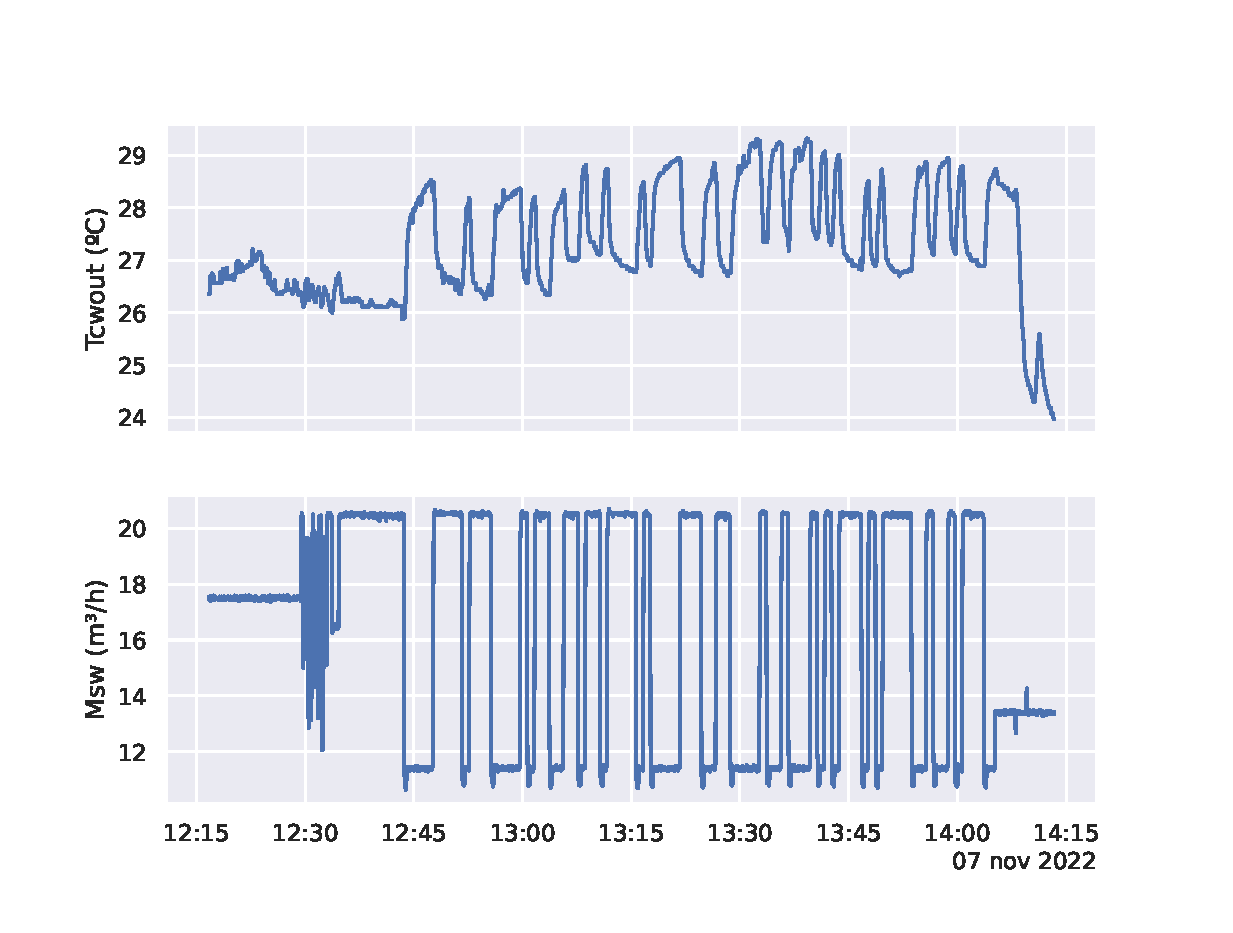
\includegraphics[width=0.48\textwidth]{figures/solarmed-std-control-tcout-ident}
    }}%
    \hspace{0.1cm}
    \subfloat[\centering
    Controller application results]{{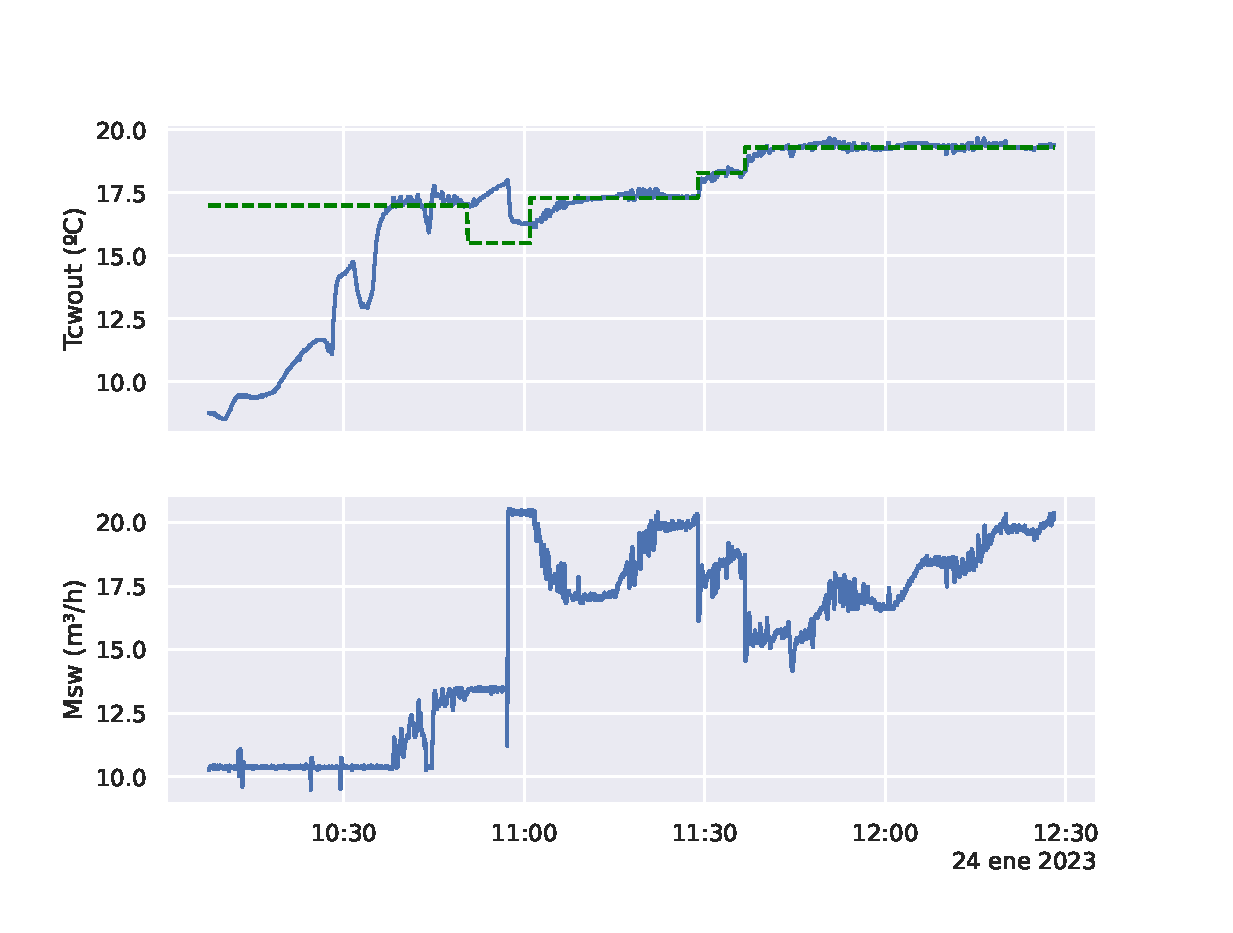
\includegraphics[width=0.48\textwidth]{figures/solarmed-std-control-tcout-control.eps}
    }}%
    \caption[Condenser outlet temperature controller implementation]{Condenser outlet temperature controller implementation. To tune the controller, the system was excited with a PRBS signal  (a), obtaining an ARX model ($n_a=20$, $n_b=49$, $n_k=5$, 96.38\% fit) using the \textit{System Identification Toolbox} from MATLAB, which allowed to extract an approximate first-order dynamic with which to tune the controller.}
    \labfig{solarmed:std:condenser-control}
\end{figure}

\subsubsection{Steady state identification}


\subsubsection{Reproducibility and the effect of the steady state duration}


%================================
\subsection{Results analysis}
Analizar los mejores puntos de operación en términos exergéticos, ...

An experimental campaign consisting on XX hours of operation, from which XX stable operation points were identified, covering a wide range of operating conditions in different seasons of the year is ...

Mostrar gráficas de color con rango de temperaturas, etc. Mapa de operación, etc.

When the system was planned, it was designed to optimize for \textit{seawater desalination} and considering \textit{process heat}\sidenote{See \refsec{solarmed:std:process}} as the only external thermal energy source. This is reflected in the higher performance values that can be observed, with low temperature difference between inlet and outlet of the heat source, whereas for brine concentration low recoveries are observed, and poor performance values are observed for the waste heat metrics

\subsubsection{Best operating strategy}

One caveat of the exergetic metrics for this particular plant, where the sink\sidenote{the simulated-fixed volume seawater} can change its conditions with significant dynamics, is that otherwise similar operating points can have different exergetic performance due to the additional cooling consumption required to maintain a certain condenser pressure / condenser outlet temperature. In order to enable fair comparison of the exergetic performance of different operating points, the cooling consumption is normalized to seawater intake at 20 $^\circ$C. 

\subsubsection{Experimental evaluation at high \glspl[format=long]{tbtLabel}}

The performance of a thermal proces, such as \gls{medLabel}, is dictated by the Carnot cycle~\sidecite{brogioli_thermodynamic_2018}, which sets the theoretical maximum efficiency for any heat engine. The efficiency of the Carnot cycle is limited by the temperature difference between the hot and cold sinks, which determine the amount of thermal energy that can be converted into useful work. An approach to bring the MED closer to its thermodynamic limit can be achieved by raising the \fullgls{tbtLabel}, which allows to increase the number of effects~\sidecite{mistry_improved_2013} while maintaining an optimal temperature drop across them. This leads to an improvement in the thermal performance of traditional desalination or an increase of the concentration factors that can be achieved\sidenote{
    This can enable \gls{zldLabel} processes and applications such us brine mining, introduced in \refch{intro:desalination}.
    }.

\begin{margintable}[]
\caption{\fullgls{rsiLabel} values and their interpretation in terms of scaling and corrosion risk~\sidecite{ryznar_new_1944}.}
    \labtab{solarmed:facility:specifications}
    \resizebox{\linewidth}{!}{%
    \begin{tabular}{cl}
    \toprule
    RSI > 9 & Severe corrosion \\
    7.5 < RSI < 9 & Heavy corrosion \\
    7 < RSI < 7.5 & Significant corrosion \\
    6 < RSI < 7 & Stable water \\
    5 < RSI < 6 & Moderate to light scaling \\
    4 < RSI < 5 & Severe scaling \\
    \bottomrule
    \end{tabular}
}
\end{margintable}


In practice, the \gls{tbtLabel} in \gls{medLabel} is limited to 70$^\circ$C since, as can be seen in \reffig{solarmed:std:tbt-pretreatment}, higher \glspl{tbtLabel} promote the precipitation of divalent ions, which are deposited in the form of incrustations in the surface of the heat exchange surfaces, thus reducing heat transfer efficiency~\sidecite{el-dessouky_fundamentals_2002}. In the figure it can be observed how for un-treated feedwater (left) this risk of precipitation is present at almost any temperature in terms of \gls{rsiLabel} due to its composition (\textit{seawater} in center bar plot). A nanofiltration pre-treatment is used to selectively remove the divalent ions while leaving relatively unaffected the components to be separated in the \gls{medLabel} process, \ie NaCl. This allows the operation of MED processes at higher TBTs or higher feed concentration, with only severe scaling above 80$^\circ$C and $\approx$ 100 g/kg.

In Table XX four operation points are compared. Two of them receive heat at 68$^\circ$C, while they differ in the feedwater flow rate, one at a high level (8 m$^3$/h) and the other at a low level (5 m$^3$/h). The other two operation points receive heat at 89$^\circ$C and same variation for the feedwater flow rate. The first two operation points result in an approximate \gls{tbtLabel} of 61.5$^\circ$C while the last two operation points have an approximate \gls{tbtLabel} of 79.2$^\circ$C. 

\begin{figure*}[h!]
    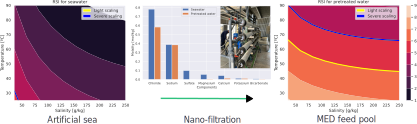
\includegraphics[]{figures/solarmed-std-tbt-pretreatment.png}
    \caption{\gls{rsiLabel} values as a function of temperature and concentration before (left) and after (right) pre-treatment using nanofiltration.}
    \labfig{solarmed:std:tbt-pretreatment}
\end{figure*}

The first inmediate observation is that contrary to what stated in the introduction, the performance of the plant does not improve with higher heat source temperatures, this can be explained by the fact that the increase in the heat source temperature is not taken advantage of by introducing more effects, which would allow\sidenote{With limitations, on each effect a considerable exergy is destroyed. It has been shown than after XX effects GOR figures ...}.

Another observation is that the concentration achieved in 

\begin{figure}
    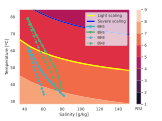
\includegraphics[width=.8\textwidth]{figures/solarmed-std-tbt-results.png}
    \caption{Temperature and concentration evolution for operation points at each effect in the MED plant. Surface represents the \gls{rsiLabel}.}
    \labfig{solarmed:std:tbt-results}
\end{figure}


Using a physical model of the plant\todo{referenciar al apéndice donde se ponga el modelo}, a better insight into the working conditions of the plant can be obtained. The model is based on the energy and mass balances of the system, and it is used to estimate different outputs at the effect level, such as the temperature and pressure of the vapor, the distillate production, and the brine concentration. This allows to analyze the concentration evolution and visualize it as shown in \reffig{solarmed:std:tbt-results}

Comentar RSI, y por último dar una idea de por qué se cree que no se alcanzan factores de concentración más elevados a pesar de subir la temperatura.

An explanation as to why the concentration factor seems limited past XX, is the boiling point elevation of the brine, which increases with its concentration, this means that the temperature difference between the brine and the vapor is reduced, which in turn reduces the driving force for heat transfer. This effect adds up, low vapor production on one effect means a diminished force for heat transfer to the next effect, which in turn reduces the vapor production on that effect, and so on.

Finally, in order to determine whether the hight temperature operation points have produced scaling, a control test was performed before the hight temperature tests, and after 30 hours of high temperature operation, repeated. \reftab{} shows the evaluation result for each control test. The results show that the scaling risk is low, with no significant degradation of any performance metric 


\section{Conclusion}


% Sobre las métricas

% Sobre la metodología

% Sobre los resultados a alta temperatura


% \setchapterpreamble[u]{\margintoc}
\chapter{Influence of increasing Top Brine Temperature on MED performance}
\labch{solarmed:tbt}
% \setchapterpreamble[u]{\margintoc}
\chapter{Towards the optimal coupling and operation of a solar driven \gls{medLabel} system}
\labch{solarmed:optimization}

\tldrbox{
    This chapter describes a method to develop an operational strategy enabling
    the seamless integration of a solar driven \gls{medLabel} system in an
    autonomous and optimal manner, including decisions on when to start or stop
    each subsystem and how to regulate them during operation.

    The method is based on a hierarchical control approach consisting of three
    layers, where the upper operation plan solves a \gls{minlpLabel} problem.
    Results for a week long simulation of the system are compared against two
    alternative strategies: a baseline operation and only operation
    optimization strategies show that the proposed method is able to
    significantly increase the water production by XX \% by taking full
    advantage of the solar resource and flexibility of the thermal storage.    
}

%===================================
%===================================
\section{Introduction}

% Estado del arte de la optimización de procesos de desalación térmica
LRoca, Carballo, Juan Diego

% Contribución

% Estructura del capítulo

%===================================
%===================================
\section{Problem description}
\labsec{solarmed:optimization:problem-description}

The behavior of the \gls{solarmedLabel} process is controlled by acting on two
components, a discrete (operation state) and a continuous one (process variables).

The goal is to design an operational strategy that enables the seamless
integration of both subsystems in an autonomous and optimal manner, including
decisions on when to start or stop each subsystem and how to regulate them
during operation. Therefore, considering the whole system as a
\fullgls{minlpLabel} optimization problem\sidenote{See
\nrefsec{intro:optimization:minlp_problems}} that aims to maximize the water
production while minimizing the (electrical) consumption of the
system. Decisions on when to
operate the system are weighted considering an optimization horizon, approximating the
operation strategy of the system to the optimum:\sidenote{In general $q$ represents flow
rates while $T$ are temperatures. \reffig{solarmed:process-diagram} can be
consulted for subscript reference.}

\marginnote[*5]{$\forall i = 1 \ldots n_{steps}$ is a notation to indicate that
    a condition must be held at every step $i$ in the optimization horizon
    ($n_{steps}$).\\ Bold variables represent vectors.}

\problemdefinitionbox{\gls{solarmedLabel}}{
    \begin{equation*}
        \min_{\mathbf{x},\, \mathbf{e};\, \boldsymbol{\theta}} \quad J = f(\mathbf{x}, \mathbf{e}; \boldsymbol{\theta}) = \sum_{i=1}^{n_{steps}} \left( J_{e,i}-J_{w,i} \right)
    \end{equation*}

    \textbf{with}:
    \begin{align*}
        \quad for\: i &= 1 \ldots n_{steps}: \\
        & \quad J_{w,i}=q_{d,i} \cdot P_{w,i}\:\text{if \textit{valid operation} else 0} \\
        & \quad J_{e,i} = C_{e,i} \cdot P_{e,i} \\
        & \quad q_{d,i},\,C_{e,i},\,\text{valid operation}=\text{solarmed model}(x_{c,i}, x_{p,i}, ...)
    \end{align*}
    \begin{itemize}
        \item Decision variables
        \[
        \mathbf{x} = [\mathbf{med_{mode}},\,\mathbf{sfts_{mode}},\,\mathbf{q_{sf}},\,\mathbf{q_{ts,src}},\,\mathbf{q_{med,s}},\,\mathbf{q_{med,f}},\,\mathbf{T_{med,s,in}},\,\mathbf{T_{med,c,out}}]
        \]
        where $\mathbf{x}_{nx \times \sum{n_{updates,xi}}}=[x_{1,i},\allowbreak\;
        \ldots,x_{1,n_{updates,x_{1}}},\allowbreak\; \ldots,x_{n_x, n_{updates,
        x_{nx}}}]$
        % where $\mathbf{x}=[x_{1,1},\,\ldots\, x_{1,n_{steps}},\, \ldots,\,
        % x_{n_{x},n_{steps}}]$
        
        \item Environment variables
        \[
        \mathbf{e} = [\mathbf{I},\,\mathbf{T_{amb}},\, \mathbf{P_e},\, \mathbf{P_{w}}]
        \]
        where $\mathbf{e}=[e_{1,1},\,\ldots\, e_{1,n_{steps}},\, \ldots,\,
        e_{n_{e},n_{steps}}]$
        
        \item Fixed parameters ??
        \[
        \theta = [R_p = 1,\, R_s = 0,\, \omega_{\text{dc}} = 0]
        \]

    \end{itemize}

    \textbf{subject to}:
    \begin{itemize}
        
        \item Box-bounds
        \begin{itemize}
            \item $\mathbf{med_{mode}} \in [0,1] \subset \mathbb{Z}$
            \item $\mathbf{sfts_{mode}} \in [0,1] \subset \mathbb{Z}$
            \item $\mathbf{q_{sf}} \in [\underline{q_{sf}}, \overline{q_{sf}}] \subset \mathbb{R}$
            \item $\mathbf{q_{ts,src}} \in [\underline{q_{ts,src}}, \overline{q_{ts,src}}] \subset \mathbb{R}$
            \item $\mathbf{q_{med,s}} \in [\underline{q_{med,s}}, \overline{q_{med,s}}] \subset \mathbb{R}$
            \item $\mathbf{q_{med,f}} \in [\underline{q_{med,f}}, \overline{q_{med,f}}] \subset \mathbb{R}$
            \item $\mathbf{T_{med,s,in}} \in [\underline{T_{med,s,in}}, \overline{T_{med,s,in}}] \subset \mathbb{R}$
            \item $\mathbf{T_{med,c,out}} \in [\underline{T_{med,c,out}}, \overline{T_{med,c,out}}] \subset \mathbb{R}$
        \end{itemize}
    \end{itemize}

    \textit{valid operation} conditions, $\forall i = 1 \ldots n_{steps}$:
    \begin{itemize}
        \item $T_{sf,out} \le \overline{T_{sf,out}}$
    \end{itemize}
}

Where the objective is to minimize the cumulative cost of operation ($J$).
Fresh water ($q_{med,d}$) sold ($J_w$) at price $P_w$ is the negative term
while electrical consumptions ($C_e$) at price $P_e$ make up the positive cost
term ($J_e$). The benefit ($B$) of operation is simply the inverse of the cost
of operation.

The environment is represented by the vector $\mathbf{e}$, which includes the
global solar irradiance ($\mathbf{I}$), ambient temperature
($\mathbf{T_{amb}}$), and the prices of water ($\mathbf{P_w}$) and electricity
($\mathbf{P_e}$).

The decision vector $\mathbf{x}$ is composed of the decision variables for both
the discrete and the continuous space. Two decision variables are defined to
manipulate the discrete state of each subsystem defined in
\refsec{solarmed:modelling:discrete}: $\text{med}_{\text{mode}}$ and
$\text{sfts}_{\text{mode}}$. These binary ($\subset \mathbb{Z}$) variables
establish whether the particular subsystem is active ($x_i=1$) or inactive
($x_i=0$). This is directly related to the operation state of the particular
subsystem\sidenote{As defined in
Tables~\ref{tab:solarmed:modelling:sfts_fsm_states} and
\ref{tab:solarmed:modelling:med_fsm_states}}\sidenote{Once the values for these
decision variables are provided, the low-level control layer is in charge of
safely transitioning between operation states \eg $med_{mode}: 0 \rightarrow
1$, med state: \textit{off} $\rightarrow$ \textit{generating vacuum}
$\rightarrow$ \textit{starting-up} $\rightarrow$ \textit{active}} and accounted
for in the models by the integrated finite-state machines as explained in
\refsec{solarmed:modelling:discrete}. For the continuous space, the decision
variables include the ones that define the operating conditions (\ie operation
point) of the \gls{medLabel} system, and the two recirculation flow rates that
determine the conditions of the heat source ($q_{sf}$, $q_{ts,src}$).

%================================
%================================
\subsection{Implementation discussion}
\labsec{solarmed:optimization:implementation}

%==============================
\subsubsection{On the constraint handling}
\labsec{solarmed:optimization:constraints-discussion}

The reader might notice that no constraints are explicitly defined in the
problem definition. This is because the constraints are implicitly defined in
the model equations, which are used to evaluate the objective function. This
design decision is motivated to avoid the need for a constraint-handling
capable optimization algorithm, limiting the choice for an already complex
\gls{minlpLabel} problem\sidenote{See
\nrefsec{intro:optimization:constraints} for a more detailed discussion on the
topic}. Specifically, two aspects demand further consideration:

\begin{enumerate}
    \item The decision value for the \gls{medLabel} outlet condenser
    temperature ($T_{med,c,out}$) is not a direct input to the system, but rather a
    setpoint to be followed by a low-level control loop by manipulating the cooling
    water flow rate ($q_{med,c}$). This input might saturate and thus not be
    able to achieve the desired setpoint. In this case, a new value for the
    decision variable is computed, which is the minimum value that can be
    achieved (with $\overline{q_{med,c}}$). 
    
    In this case, the value used in the \gls{solarmedLabel} and the output from
    the optimization to the low-level control layer would be the validated
    value for $T_{med,c,out}$. No additional actions are needed.

    \item In the solar field, in order to not constantly interrupt the
    evaluation due to the solar field temperature going above
    $\overline{T_{sf,out}}$ (120 $^\circ$C), the model saturates this
    temperature when going above and sets a flag. The limitation of this approach
    is that when there is low energy demand from the
    load, and likely because it favors energy transfer in the heat exchanger
    \sidenote{greater temperature difference in primary side instead of greater mass
    flow rate with its associated increase in pumping power},
    the optimizer tends to minimize the solar field flow, and systematically
    lets the solar field outlet temperature reach the limit. To avoid this
    situation, the positive term of the objective function is nullified in
    iterations where the constraint is not met.
    
    Here, in order to ensure \textit{valid operation} the fitness function is
    manipulated to de-incentivize decision variable values that lead to
    unfeasible operation. 

\end{enumerate}

\subsubsection{On the prediction horizon}
\labsec{solarmed:optimization:decision_variables-discussion}

The problem is designed as an optimization problem with a shrinking
horizon\marginreminder[*-2]{Shrinking horizon optimization}{
An optimization where the horizon end is fixed, and as time progresses, the
start of the horizon moves forward.\footnote{See
\nrefch{intro:optimization}}
}. The horizon size should be large enough so that
decisions on how to operate the system are made with perspective, taking into
account how they will affect the system in the future, but not so large that
current decisions have no impact on the far future, and making the problem dimensionality become unmanageable. 

For this case study, this parameter should be chosen based
on the hours of capacity of the thermal storage to operate the \gls{medLabel} system.

The thermal storage capacity is XXX which allows the system to operate with no
supply from the solar field for up to XX hours. This means that depending on
the charge state of the thermal storage, the system could start operation
independently of the irradiance conditions, or operate at different levels of
temperature. Considering this the optimization horizon,
in time units, chosen was 36 hours. This means that if the optimization is evaluated at
5:00 on day 1, the fitness function is evaluated until 19:00 of day 2 \ie
including the end of operation for day 2. 

%===================================
%===================================
\subsubsection{On solving the optimization problem}
\labsec{solarmed:optimization:solving-discussion}

Solving the optimization problem for this \fullgls{minlpLabel} formulation
presents significant challenges due to the combinatorial nature of the integer
decision variables~\sidecite{grossmann_advanced_2021}. As shown in
\reffig{solarmed:optimization:decision_tree}, each combination of integer
decisions, such as the operational modes of the separation subsystem
($med_{mode}$) and the solar field thermal storage subsystem ($sfts_{mode}$),
leads to a different system trajectory along the prediction
horizon\sidenote{This will be referred to as: \textbf{operation plan}}.

The number of possible operation trajectories increases exponentially with both
the number of integer variables ($n_{xi}$) and the number of decision updates
($n_{\text{updates}, xi}$), following the expression\sidenote{For example: 
$n_{\text{updates}, \forall xi}=6 \rightarrow n_{problems} = 64$,
$n_{\text{updates}, \forall xi}=24 \rightarrow n_{problems} = 16\,777\,216$}:

\begin{equation}
    \labeq{solarmed:optimization:n_problems}
    n_{\text{problems}} = n_{xi}^{n_{\text{updates}, xi}}.
\end{equation}

This exponential growth makes the search space extremely large and complex.

An important design consideration when solving the optimization problem is
whether the sequence of integer decisions (\ie, operational mode transitions
over time) is predefined or whether the optimization algorithm is allowed to
explore the decision tree freely and determine the optimal sequence. The latter
case requires more computational effort but allows for potentially better-performing
solutions by dynamically adjusting to system conditions.


\subsubsection{On the decision variables update frequency}
\labsec{solarmed:optimization:decision_variables-discussion}

Apart from the integer decision variables, if a fixed decision variable update
frequency is chosen for all continuous decision variables, the size of the
decision vector for a large horizon like the one chosen can become large with
diminishing returns. Instead, a new design parameter is introduced: the number
of decision variable updates ($n_{updates, x_i}$) for each decision variable in
the optimization problem.

Thus, the decision vector is formed by each individual decision variable repeated as
many times as updates for it:
\[ 
    X_{nx \times\sum{n_{updates,xi}}}=[x_{1,k},\allowbreak\;
    \ldots,x_{1,n_{updates,x_{1}}},\allowbreak\; \ldots,x_{n_x, n_{updates,
    x_{nx}}}]
\]

The number of updates of the decision variable ($n_{updates, x_i}
\in [1,n_{steps}]$) can be chosen individually. More updates are assigned to
variables regulating faster dynamics ($q_{sf}$, $q_{ts,src}$), and these
updates of the decision variables are evenly distributed throughout the \textit{active}
period of the subsystem within the horizon. This is a crucial design
consideration since otherwise the limited number of updates would be assigned
to long inactive periods (between end of operation in day 1 and start on day
2). 
\begin{marginfigure}[-10cm]
    \includegraphics[]{figures/solarmed-optimization-decision_tree.png}
    \caption{Decision tree resulting from the combinatorial nature of the integer part of the optimization problem. Text in nodes represents system states.}
    \labfig{solarmed:optimization:decision_tree}
\end{marginfigure}

It also means that the continuous component of the decision vector can only be
assigned timestamps after the integer part is defined.
Once timestamps are associated with each decision variable, the decision vector
values can be resampled to match the desired sampling time of the optimization
problem. This is done by forward filling \cite{hyndman_forecasting_2021}
the values of the decision vector until the next update time. 

%===================================
\section[]{Proposed optimization strategy}[Proposed strategy]
\labsec{solarmed:optimization:strategy}

A hierarchical control approach (see
\reffig{solarmed:optimization:architecture}) was chosen consisting of
three layers: operation plan, operation optimization, and control.
This scheme was chosen for two main reasons. On the one hand, the time scales
of the different aspects of the operation of the system (operation mode
changes, process variables setpoint changes, regulatory control, respectively)
can differ substantially. Secondly, it allows to abstract process complexity
from the more computationally demanding upper layers by allocating it into the
downstream layers. The operation plan layer makes decisions for the \textit{operation
modes}, the operation optimization layer sets the setpoints given to the
continuous \textit{process variables} that are to be followed by the low-level
regulatory control layer.

\begin{marginfigure}[-3.5cm]
    \includegraphics[]{figures/solarmed-optimization-architecture.png}
    \caption{Proposed optimization strategy architecture}
    \labfig{solarmed:optimization:architecture}
\end{marginfigure}

Both operation plan and operation optimization layers share the same underlying
problem structure, the difference being that the operation plan layer evaluates
a predefined library of $\text{n}_{\text{problems}}$ combinations of the binary
decision variables $\text{med}_{mode}$ and $\text{sfts}_{mode}$ twice; once to
decide the operation start, and another to end operation. The operation
optimization layer periodically solves a single \gls{nlpLabel} problem with the
selected values for these two variables fixed. They are further described in
the following sections.

% This layered optimization procedure is illustrated in
% \reffig{solarmed:optimization:architecture} where it can be seen that the
% proposed strategy is composed by an ordered sequence of evaluations of the
% different layers. 

\section{Operation Plan Layer Description}

\marginnote{The number of updates available for each integer variable
$n_{updates,xi}$ will be interchangeably referred to as \fullgls{dofLabel}.}

This layer determines the integer decision variables of the \gls{minlpLabel}
problem, namely, the sequence of operation modes producing an operation plan. 
To make the problem computationally
tractable, only a limited number of combinations, $n_{problems}$, are
evaluated. This transforms the mixed-integer problem into a simpler form by
moving the integer variables from the decision to the environment space.
In effect, the original \textbf{\gls{minlpLabel}} is decomposed into a library
of \textbf{n\gls{nlpLabel}} problems that are individually
evaluated\sidenote{\textbf{\gls{minlpLabel}} $\rightarrow$ \textbf{n\gls{nlpLabel}}}.

% As mentioned, two evaluations of this layer are performed at different times:
% one to plan subsystem start-up, and another to schedule shutdown.  

To improve robustness, the layer can be evaluated multiple times ($n_{evals}$)
under different scenarios—typically reflecting variations in forecasted
environmental conditions. The final operation plan is selected as the best
compromise across these scenarios.

The time required to perform this layer’s computation is denoted
$\Delta t_{eval,plan}$.

\subsection{Candidate problems generation}

Given the available computational resources and the complexity of the objective
function, it has been found feasible to evaluate in the order of $n_{problems}
\sim 100$ candidate combinations. This constraint informs how many
\fullgls{dofLabel} (\ie number of updates available for the operation modes)
can be defined by using \refeq{solarmed:optimization:n_problems}. The
particular design choice for the number of updates per subsystem is shown in
\reftab{solarmed:optimization:dof}. In total, 101 distinct operation plans are
generated for the start-up evaluation and 144 for the shutdown\sidenote[][*-5]{Notice
the total number does not match exactly \refeq{solarmed:optimization:n_problems} since
special cases are added (subsystem inactive)}.

\begin{table}[htbp]
\centering
\caption{Operation plan. Start-up (1) and shutdown (2) degrees of freedom for changes in the operation state.}
\labtab{solarmed:optimization:dof}
\resizebox{\textwidth}{!}{%
\begin{tabular}{lrrccccccclc}
\cline{2-12}
 & \multicolumn{1}{c}{\multirow{3}{*}{\textbf{Subsystem}}} &  & \multicolumn{7}{l}{\textbf{Degrees of freedom}} &  & \multirow{3}{*}{$\textbf{n}_{\textbf{problems}}$} \\ \cline{4-10}
 & \multicolumn{1}{c}{} &  & \multicolumn{3}{l}{Day 1} &  & \multicolumn{3}{l}{Day 2} &  &  \\ \cline{4-6} \cline{8-10}
 & \multicolumn{1}{c}{} &  & Start &  & Stop &  & Start &  & Stop &  &  \\ \cline{2-2} \cline{4-4} \cline{6-6} \cline{8-8} \cline{10-10} \cline{12-12} 
\multirow{2}{*}{Evaluation: Start-up (1)} & sfts &  & 3 &  & 3 &  & 1 &  & 1 &  & \multirow{2}{*}{101} \\
 & med &  & 3 &  & 3 &  & 1 &  & 1 &  &  \\ \cline{2-12} 
\multirow{2}{*}{Evaluation: Shutdown (2)} & sfts &  & - &  & 3 &  & 2 &  & 2 &  & \multirow{2}{*}{144} \\
 & med &  & - &  & 3 &  & 2 &  & 2 &  &  \\ \cline{2-12} 
\end{tabular}%
}
\end{table}


\subsection{Update times generation}

Up to this stage the operation plans generated just consist of a list of ones
and zeros for each subsystem, indicating whether the subsystem is active or
inactive in the particular update. The next step is to assign the operation
mode updates to specific time instants, which then can be resampled to match
the desired sampling time of the optimization problem\sidenote{As with the
continuous component of the decision vector, this is done by forward filling
\cite{hyndman_forecasting_2021} the values of the decision vector until the
next update time. This is also known as \textit{Last Observation Carried Forward}}.

In order to maintain the solution close to the optimal one, while keeping the
number of problems reasonable, decision updates are distributed throughout the
prediction horizon at strategic time instants. Since the case study system is
fundamentally a solar process, the operation is strongly dependent on the
irradiance availability, and thus operation changes are likely to take place at
the start and end of the solar day. 

The operation mode updates are distributed temporally as shown in
\reffig{solarmed:optimization:operation_plan} (b) depending on the number of
updates available (\gls{dofLabel}). These update times are dependent on the
solar irradiance profile and are bounded by lower- and upper-level thresholds.
Depending on the plan action (start-up or shutdown), they are named early-late
start or early-late stop thresholds, respectively.

In \reffig{solarmed:optimization:operation_plan} (b) up to three \gls{dofLabel}
are visualized. If only one update is available, the update time is set at the
mean of the early and late thresholds. If two \gls{dofLabel} are available, for
the \gls{sftsLabel} subsystem, they are placed halfway between the early
threshold and the mean, and the late threshold and the mean, respectively. For
the \gls{medLabel} subsystem, updates are delayed. Finally, with three
\gls{dofLabel}, updates for the \gls{sftsLabel} subsystem are placed at the
early, mean and late thresholds, while for the \gls{medLabel} subsystem, the
leftmost and rightmost updates are shifted to the left and right, respectively.
If more updates for the particular action are available \ie \gls{dofLabel},
additional thresholds can be added.

\begin{figure*}
    \centering
    \subfloat[\centering Computation timeline]{{\includegraphics[width=0.48\linewidth]{figures/solarmed-optimization-timeline.png}}}%
    \hspace{0.01\linewidth}
    \subfloat[\centering Operation mode updates time distribution]{{\includegraphics[width=0.48\linewidth]{figures/solarmed-optimization-updates_distribution.png}}}%
    \caption[Operation plan layer computation and updates distribution]{Operation plan layer computation and updates distribution. The yellow line represents the irradiance illustrating the solar day.}%
    \labfig{solarmed:optimization:operation_plan}
\end{figure*}


Given a number of updates per subsystem and the update times assigned. The
potential operation time change candidates are defined as:

\[
    t_{mode-change,candidates} = [t_0,\, t_1,\, \ldots,\, t_{max(n_{updates,\forall x_i})}]
\]

Ordered in ascending order, where $t_0$ is the earliest potential operation
change time and $t_{max(n_{updates,\forall x_i})}$ is the latest potential
operation change time. Based on this definition, the earliest potential
subsystem start-up would be at $t_{\uparrow, candidates}(0)$. Similarly, the earliest
potential shutdown would be at $t_{\downarrow, candidates}(0)$.

\subsubsection{Start-up}
\labsec{solarmed:optimization:operation_plan:start-up}

The most important aspect of this evaluation is to find the right time to bring
the subsystems online, and secondary is to provide a preliminary estimate for
their shutdown timing.

This is the first evaluation of the proposed methodology (see
\reffig{solarmed:optimization:architecture}) and is computed ahead of the first
potential operation mode change (\reffig{solarmed:optimization:operation_plan}
(a) - \textit{start-up}), with enough lead time to complete the analysis before
any potential change in operation mode ($t_{\uparrow,candidates}(0)$):

\[
    t=t_{\uparrow,candidates}(0) - (\Delta t_{eval,plan}\times n_{evals})
\]

Being the earliest evaluation, it has the longest prediction horizon and thus
the highest predicted variables uncertainty. As a counterpart, as shown in
\reffig{solarmed:optimization:operation_plan} (a), this early evaluation start
allows sufficient computation time, even several hours in advance, to perform
several evaluations. Specifically three evaluations ($n_{evals}$) are performed: a
nominal scenario with the forecasted environmental conditions, a pessimist one
with a 20\% decrease in the expected solar irradiance and finally an optimist
one with a 20\% increase in the expected solar irradiance.


\subsubsection{Shutdown}

A second evaluation is performed later in the day (see
\reffig{solarmed:optimization:architecture}), before system shutdown. This
aims to determine the most suitable time to stop operations using the most
recent system state information. It includes \gls{dofLabel} regarding the
operation schedule for the following day, allowing the shutdown decision for
day 1 to account for its impact on the start and end times of day
2\sidenote{See \reftab{solarmed:optimization:dof}}. 

Only one evaluation is performed, as the uncertainty in the prediction horizon
is significantly lower than in the start-up evaluation. It is evaluated in
parallel to the operation optimization layer and just before the earliest
expected shutdown time of the subsystems from
\nrefsec{solarmed:optimization:operation_plan:start-up},
$t_{\downarrow,candidates}(0)$, considering subsystem shutdown.

\[
    t=t_{\downarrow,candidates}(0) - (\Delta t_{eval,plan} \times some number)
\]

Once computed the integer decision are updated in this layer. The faster the
computation the better, since it will allow the operation optimization layer to
optimize operation for the actual shutdown time and adapt accordingly.


\section{Operation optimization layer description}

As mentioned, this middle layer establishes the setpoints for the continuous
process variables, \ie the continuous part of the \gls{minlpLabel} problem. The
operation optimization layer evaluates periodically, with a sample time
$T_{eval,optim}$, a \gls{nlpLabel} problem where the integer decision variables
are fixed to the values provided by the operation plan layer\sidenote{It is
exactly equivalent to the operation plan layer problem, just making
$n_{problems}=1$}. It uses the latest available state of the system and
environment predictions to evaluate the objective function.

The layer computation time is named $\Delta t_{eval,optim}$.



\begin{kaobox}[title=\gls{solarmedLabel} optimization methodology]

    \begin{enumerate}
        \item Generate operation mode change candidates based on the available
        updates per subsystem and irradiance thresholds.
        \item Before the first potential operation change and considering the
        evaluation time, $t=t_{\uparrow,candidates}(0) - (\Delta
        t_{eval,plan}\times n_{evals})$, evaluate the operation plan layer to
        establish the operation start of the subsystems and an estimation of
        when to stop.
        
        \item Before the established startup and considering the layer evaluation time, $t=t_{\uparrow} - \Delta
        t_{eval,optim}$, start evaluating the operation optimization layer
        periodically ($T_{eval,optim}$) to establish the setpoints for the
        continuous process variables.

        \item Before the earliest subsystem projected shutdown and considering
        the operation optimization layer evaluation time,
        $t=t_{\downarrow,candidates}(0) - \Delta t_{eval,plan}$, evaluate
        the operation plan layer, in parallel to the operation optimization layer,
        to establish the shutdown time of the subsystems.

        \item Continue evaluating the operation optimization layer periodically
        ($T_{eval,optim}$) until the last subsystem is shutdown.
    \end{enumerate}

\end{kaobox}

%----------------------------------------------------------------------------------------
%	COMBINED COOLING
%----------------------------------------------------------------------------------------
\pagelayout{wide} % No margins
\addpart{Optimal water and electricity management in a combined cooling system}
\pagelayout{margin} % Restore margins

\section*{Introduction}
\addcontentsline{toc}{section}{Introduction}

\section*{TL;DR}
\addcontentsline{toc}{section}{TL;DR}

\section*{Derived scientific contributions}
\addcontentsline{toc}{section}{Derived scientific contributions}
\setchapterpreamble[u]{\margintoc}
\chapter{Modelling of a combined cooling system}
\labch{solhycool:modelling}

\tldrbox{
    This chapter describes the steady-state modelling of the different
    components of a combined cooling system, mainly a \gls{wctLabel} and a
    \gls{dcLabel}. Different alternatives are presented: from physical models
    to data-driven approaches, including the generation of samples for
    data-driven models trained using data from a physical model. Models are
    also developed for the other components of the system and finally it is
    shown how they are integrated into a complete system model. The complete
    system model interface is defined at \refmod{mod:cc} and a block diagram is
    presented in \reffig{cc:modelling:complete-model-diagram} including all
    relevant variables.
}

\section*{Introduction}

% Estructura a seguir:

% Estado del arte + Contribución del capítulo + Estructura del capítulo

% Introducción de artículo: Wet cooling tower performance prediction in CSP
% plants: A comparison between artificial neural networks and Poppe’s model
In order to study the potential advantages of making use of a combined
cooling\todo{ Ahora mismo esta introducción es demasiado parecida al TL;DR, hay
que distinguirla } system, it is first necessary to develop the modelling of
its components. Since the objective is performance prediction, this chapter
focuses on the steady state modelling of the combined cooler main components,
\ie the \gls{wctLabel} and the \gls{dcLabel}. More specifically, the aim is to
compare two modelling strategies: that based on physical equations
(\refsec{intro:modelling:first-principle}) and that based on black box models
(\refsec{intro:modelling:data-driven}) such as \glspl[format=long]{annLabel},
in order to see which one is more suitable for its integration in the
optimization of the complete process. 

This chapter presents a comparison between the two modelling approaches, at
steady state and with a focus on optimization applications, in terms of
predictive capabilities, experimental and instrumentation requirements,
execution time, implementation and scalability. A sensitivity analysis is
performed to further analyze and compare each case study. It also presents and
evaluates all relevant aspects of interest in the development of such models,
specifically for \gls{annLabel}s, model configuration, architecture and
topology are discussed. Other system components are also described in
\nrefsec{cc:modelling:other-components} and finally their integration is
discussed in \nrefsec{cc:modelling:complete-model}.


%===================================
%===================================
\section{Wet cooler}
\labsec{cc:modelling:wct}

% Estado del arte en modelado \gls{wctLabel}
%================================
% \subsection{Wet cooling tower modelling}

In the case of the models based on physical equations, the analysis of wet
cooling towers has its origin in~\sidecite{merkel_verdunstungskuhlung_1925}, in
which the theory for their performance evaluation was developed. Merkel
proposed a model based on several assumptions to simplify the heat and mass
transfer equations to a simple hand calculation. However, these assumptions
mean that Merkel's method does not reliably represent the physics of the heat
and mass transfer process in a cooling tower. This was already stated by
Bourillot~\sidecite{bourillot_hypotheses_1983} who concluded that the Merkel
method is simple to use and can correctly predict cold water temperature when
an appropriate value of the coefficient of evaporation is used. However, it is
insufficient for the estimation of the characteristics of the warm air leaving
the fill and for the calculation of changes in the water flow rate due to
evaporation. Jaber and Webb~\sidecite{jaber_design_1989} developed the
equations necessary to apply the effectiveness-NTU\sidenote{The
effectiveness-NTU method estimates how well a heat exchanger transfers heat by
comparing the actual heat transfer to the maximum possible, using a parameter,
\gls{ntuLabel}, that reflects its size and flow characteristics.} method
directly to counterflow or crossflow cooling towers. This approach is
particularly useful in the latter case and simpler compared to a more
conventional numerical procedure. Notice that the effectiveness-\gls{ntuLabel}
method is based on the same simplifying assumptions as the Merkel method. On
the other hand, Poppe and Rögener~\sidecite{poppe_berechnung_1991} developed
the Poppe method. They derived the governing equations for heat and mass
transfer in a wet cooling tower and did not make any simplifying assumptions as
in the Merkel theory, which makes it a very precise model. As a matter of fact,
predictions from the Poppe formulation have resulted in values of evaporated
water flow rate that are in good agreement with full scale cooling tower test
results~\sidecite{kloppers_critical_2005}. This model has already been used for
the evaluation of the thermal performance of solar power plants using different
condensation systems (wet, dry and hybrid system), as can be found in Cutillas
et al.~\sidecite{cutillas_energetic_2021}. 

In the case of black box models, numerous authors in the literature have
designed \gls{annLabel} models for \gls{wctLabel} with different objectives,
such as performance prediction, simulation and optimization. One of the first
works in this area is the one described in~\sidecite{hosoz_performance_2007}
where an \gls{annLabel} model was developed to predict the performance of a
forced-counter flow cooling tower at lab scale. In this case, the input
variables were the dry bulb temperature, the relative humidity of the air
stream entering the tower, the temperature of the water entering the tower, the
air volume flow rate and the cooling water mass flow rate. The outputs of this
model were the heat rejection rate at the tower, the mass flow rate of water
evaporated, the temperature of the cooling water at the tower outlet, the dry
bulb temperature and the relative humidity of the air at the outlet of the
tower. The results obtained with a 5-5-5\sidenote{The notation $n_1$-...-$n_l$
represents the architecture of the \gls{annLabel} model, where $l$ is the
number of layers and $n_i$ are the nodes in each one of the layers.}
\gls{annLabel} demonstrated that wet cooling towers at lab-scale can be
modelled using \gls{annLabel}s with a high degree of accuracy. There are also
\gls{annLabel} models for Natural Draft Counter-flow Wet Cooling Towers
(ND\gls{wctLabel}) at lab-scale, such as the one proposed by
\sidecite{gao_artificial_2013}. In this case, the authors used a 4-8-6
\gls{annLabel} structure and considered some additional variables, such as air
gravity, wind velocity, heat transfer coefficients and efficiency as outputs.
All these works can be useful to validate the model development methodology but
may fail predicting the performance of \gls{wctLabel} at larger scale. In this
sense, special attention deserves the study carried out by
\sidecite{song_novel_2021} where an 8-14-2 \gls{annLabel} model was proposed to
predict the performance (the cooling number and the evaporative loss
proportion) of ND\gls{wctLabel}s at commercial scale. The model is based on 638
sets of field experimental data collected from 36 diverse ND\gls{wctLabel}s
used in power plants. It is a very challenging work since it covers samples
from a wide range of tower sizes and capacities being the \gls{mreLabel} below
5~\%. 

From the literature review, it can be stated that there are works based on
Poppe and \gls{annLabel} models that evaluate the main output variables of
\gls{wctLabel}s. Nevertheless, to the author knowledge, there are no studies
focused on the comparison between both modelling strategies. Also lacking is a
comprehensive analysis of the different aspects that affect the models
development and performance.


The static models presented in this section have been developed to predict two
main outputs, the water temperature at the outlet of the \gls{wctLabel},
$T_{w,o}$, and the water consumed due to evaporation losses,
$\dot{m}_{w,lost}$. The inputs variables required by both modelling approaches,
Poppe model and \gls{annLabel} models, are: the cooling water flow rate
($\dot{m}_w$), the water temperature at the inlet of the \gls{wctLabel}
($T_{w,i}$), the ambient temperature ($T_{\infty}$), the ambient relative
humidity ($\phi_{\infty}$) and the frequency percentage of the fan ($f_{fan}$)
(or its equivalence in air mass flow rate\sidenote{\gls{annLabel} uses as input
$f_{fan}$ whereas Poppe's model uses $\dot{m}_a$.}, $\dot{m}_a$).

%====================================
\subsection{Poppe model} 
\labsec{cc:modelling:wct:poppe}

The well-known Merkel number is accepted as the performance coefficient of a
wet cooling tower \sidecite{navarro_critical_2022}. This dimensionless number is
defined in \refeq{Me}, and it measures the degree of difficulty of the
mass transfer processes occurring in the exchange area of a wet cooling
tower.

\begin{equation} 
    Me = \frac{h_D a_v V}{\dot{m}_w}, 
    \labeq{Me}
\end{equation}

where $h_D$ is the mass transfer coefficient, $a_V$ is the surface area of
exchange per unit of volume and $V$ is the volume of the transfer region.

The Merkel number can be calculated using the Merkel and Poppe theories for
the performance evaluation of cooling towers. On the one hand, the Merkel
theory \sidecite{merkel_verdunstungskuhlung_1925} relies on several critical assumptions, such as the
Lewis factor (Le) being equal to 1, the air exiting the tower being saturated
with water vapour and it neglects the reduction of water flow rate by
evaporation in the energy balance. On the other hand, the Poppe theory
\sidecite{poppe_berechnung_1991}, which is the one used in this work, do not consider
simplifying assumptions, thus being the one most usually preferred. In this
theory, the authors derived the governing equations for heat and mass
transfer in the transfer region of the wet cooling tower (control volume
shown in \reffig{cc:modelling:poppe-transfer-area}) assuming a one dimensional problem. In
this figure, the red and green dashed lines indicate the fill and air-side
control volumes, respectively.

\vspace{1.5cm} 
\begin{figure}[htbp] 
    \begin{overpic}[width=10cm]{figures/poppe_control_volume.pdf} 
        \put(-3.3,26){$dz$}
        \put(13,65){$\dot{m}_w+d\dot{m}_w$} \put(14,57){$h_w+dh_w$}
        \put(15,-7){$\dot{m}_w$, $h_w$}
        \put(60.5,65){$\dot{m}_a\left(1+\omega+d\omega\right)$} \put(65,57){$h+dh$}
        \put(55,-7){$\dot{m}_a\left(1+\omega\right)$, $ h $}
        \put(44,30){$d\dot{m}_w=h_D\left(\omega_{s,w}-\omega\right)dA$}
        \put(44,22){$h_C\left(T_{w}-T\right)dA$}        
    \end{overpic} 
    \vspace{1cm} 
    \caption {Control volume in the exchange area of a wet cooling tower arrangement.}
    \labfig{cc:modelling:poppe-transfer-area}
\end{figure}

Following the detailed derivation process and simplification of the
previously-mentioned governing equations described in
\cite{navarro_critical_2022}, the major following equations for the heat and mass
transfer obtained, according to the Poppe theory, are: 

\begin{eqnarray}
    & & 
    \frac{d\omega}{dT_w} = \frac{c_{p_w}
    \frac{\dot{m}_w}{\dot{m}_a}\left(\omega_{s,w} - \omega \right)
    }{\left(h_{s,w}-h\right)+\left(\lew-1
    \right)\left[\left(h_{s,w}-h\right)-\left(\omega_{s,w} - \omega
    \right)h_v\right] -\left(\omega_{s,w} - \omega \right)h_w } \\
    & & 
    \frac{dh}{dT_w} = c_{p_w}\frac{\dot{m}_w}{\dot{m}_a}
    \left[1+\frac{\left(\omega_{s,w} - \omega  \right)c_{p_w}
    T_w}{\left(h_{s,w}-h\right)+\left(\lew-1
    \right)\left[\left(h_{s,w}-h\right)-\left(\omega_{s,w} - \omega
    \right)h_v\right] -\left(\omega_{s,w} - \omega \right)h_w}\right] \\
    & & 
    \frac{d\Me}{dT_w} = \frac{c_{p_w}  }{\left(h_{s,w}-h\right)+\left(\lew-1
    \right)\left[\left(h_{s,w}-h\right)-\left(\omega_{s,w} - \omega
    \right)h_v\right] -\left(\omega_{s,w} - \omega \right)h_w }, \label{eq:Me1}
\end{eqnarray}

where the quantity referred to as $\Me $ in Eq. \ref{eq:Me1}, is the Merkel
number calculated according to the Poppe theory. The above described
governing equations can be solved by the fourth order Runge-Kutta method to
provide the evolution of the air humidity ratio, air enthalpy and Merkel
number inside the transfer area of the cooling tower (fill). Once these
profiles are known, the amount of water lost due evaporation can be
calculated as per Eq. \refeq{mwlost}. Refer to \sidecite{navarro_critical_2022}
for additional information concerning the calculation procedure.

\begin{equation} 
    Me = \frac{h_D a_v V}{\dot{m}_w}, % \label{eq:Me} %
\end{equation}

\begin{equation}
    \dot{m}_{w,lost}=\dot{m}_a (\omega_{a,o}-\omega_{a,i})
    \labeq{mwlost} 
\end{equation}


It is important to mention that the Merkel number varies with the operation
conditions and its value can be obtained using a correlation with the
water-to-air mass flow ratio as an independent variable. One of the proposed
correlations in ASHRAE~\sidecite[*-2]{ashrae_hvac_2004} is:

\begin{equation}
    \Me = c\left({\dot{m}_w}/{\dot{m}_a}\right)^{-n}
    \labeq{cc:Me-corr}
\end{equation}

where the constants $c$ and $n$ can be obtained from the fitting of
 experimental data\sidenote[][*-1]{See \nrefsec{cc:validation:wct}}. 

%=====================================
\subsection{Samples generation for first-principles to data-driven models}

The first pair of input variables for the \gls{wctLabel} sample generation are
the wet bulb temperature ($T_{wb}$) and the difference between this temperature
and the system inlet temperature ($\Delta T_{wb-in}$). The wet bulb temperature
is used instead of the ambient temperature or the relative humidity, because as
it can be derived from the physical model, it is the most relevant
thermodynamic variable for the wet cooling tower performance. Using both the
ambient temperature and the relative humidity would lead to a larger than
necessary input space with many duplicate samples, as the wet bulb
temperature is a function of both variables. The second pair of input
variables are the cooling water flow rate ($q_{wct}$) and, following the
reasoning from the physical model, the air to water mass flow ratio
($\dot{m}_{a}/\dot{m}_{wct}$), since it is a key parameter in defining the
operating conditions of the tower. From the resulting 2D grid, valid combinations
are obtained by calculating the air mass flow rate and finding if a valid fan
speed can be obtained using an air mass flow rate to fan speed empirical
correlation.

Finally, all valid thermodynamic and operational combinations are merged into a
comprehensive sample set, enabling detailed system evaluations across a
realistic and constrained input space.

\subsection{Model interface}

\begin{modelcounter}{Wet cooling tower}
    \begin{equation*}
        T_{wct,out},\,C_{w,wct} = \text{wct\:model}(q_{wct},\, \omega_{wct},\, T_{amb},\, HR,\, T_{wct,in})
    \end{equation*}
    \labmod{wct}
\end{modelcounter}

\begin{modelcounter}{Wet cooling system model}
    \begin{align*}
        T_{wct,out},&\,C_{e},C_{w},\,T_{c,in},\,T_{c,out} = \text{wcs\:model}(q_{wct},\, \omega_{wct},\, T_{amb},\, HR,\, T_{wct,in}) \\
        % condenser model
        & T_{c,in},\,T_{c,out} = \text{condenser\:model}(q_c,\, \dot{m}_v,\, T_v) \\
        % wet cooler model
        & T_{wct,out},\,C_{w,wct} = \text{wct\:model}(q_{wct},\, \omega_{wct},\, T_{amb},\, HR,\, T_{c,out}) \\
        % electrical consumptions
        & C_{e,c} = \text{electrical\:consumption}(q_c) \\
        & C_{e,wct} = \text{electrical\:consumption}(\omega_{wct}) \\
        % totals
        & C_{e} = C_{e,wct} + C_{e,c} \\
        & C_{w} = C_{w,wct}
    \end{align*}
    \labmod{wet-system}
\end{modelcounter}


%=====================================
%=====================================
\section{Dry cooler}



%================================
\subsection{Physical model}

a\todo{Pendiente de basarse en el artículo del modelo físico del DC con Elxe}


%=====================================
\subsection{Samples generation for first-principles to data-driven models}
\labsec{cc:modelling:dc:samples}
% de muestreos seguida y mostrar la gráfica de resultados

Similar to the wet cooling tower case, setting absolute values for both the
inlet temperature and the environment temperature will lead to many unfeasible
combinations ($T_{dc,in} \le T_{db}$). So instead, values are generated for the
temperature difference, therefore, a 2D grid is constructed using combinations
of ambient/dry-bulb temperature ($T_{amb}$) and the difference between inlet
and ambient temperature (($\Delta T_{amb-in}$)). For each valid temperature
pair ($T_{amb}$, $T_{dc,in}$), additional independent variables ($q_{dc}$,
$\omega_{dc}$) are combined via a Cartesian product, resulting in a full
multidimensional grid of plausible operating points. This systematic procedure
ensures a dense and uniform sampling across all relevant input dimensions.
Finally, infeasible combinations are filtered based on physical constraints.


%incluir figura con distribución de muestras generadas

%================================
\subsection{Model interface}

\begin{modelcounter}{Dry cooler}
    \begin{equation*}
        T_{dc,out} = \text{dc\:model}(q_{dc},\, \omega_{\text{dc}},\, T_{\text{amb}},\, T_{dc,in})
    \end{equation*}
    \labmod{dc}
\end{modelcounter}
% \marginnote[*-2]{The condenser area ($A$) is a constant parameter}

\begin{modelcounter}{Dry cooling system model}
    \begin{align*}
        T_{dc,out},&\,C_{e},\,T_{c,in},\,T_{c,out} = \text{dcs\:model}(q_{dc},\, \omega_{dc},\, T_{amb},\, T_{dc,in}) \\
        % condenser model
        & T_{c,in},\,T_{c,out} = \text{condenser\:model}(q_c,\, \dot{m}_v,\, T_v) \\
        % dc model
        & T_{dc,out} = \text{dc\:model}(q_{dc},\, \omega_{\text{dc}},\, T_{\text{amb}},\, T_{c,out}) \\
        % electrical consumptions
        & C_{e,c} = \text{electrical\:consumption}(q_c) \\
        & C_{e,dc} = \text{electrical\:consumption}(\omega_{dc}) \\
        % totals
        & C_{e} = C_{e,dc} + C_{e,c} \\
    \end{align*}
    \labmod{dc-system}
\end{modelcounter}


%=====================================
%=====================================
\section{Other components}
\labsec{cc:modelling:other-components}


%================================
\subsection{Electrical consumption}

Electrical consumption is modelled with polynomial regressions of order 3 from
experimental data:

\begin{modelcounter}{Electrical consumption}
    \begin{align*}
        C_{e} &= \mathrm{electrical\:consumption\:model}(x) \\
        & C_{e} = p_1 \cdot x^3 + p_2 \cdot x^2 + p_3 \cdot x + p_4
    \end{align*}
    \labmod{electrical-consumption}
\end{modelcounter}

where \(C_e\) represents the electrical consumption, and \(x\) is the input
variable (e.g., the recirculated cooling water flow rate, particular cooler fan
speed, etc.). The coefficients \(p_i\) correspond to a polynomial regression
and must be calibrated individually for each component.


%================================
\subsection{Surface condenser}
\labsec{cc:modelling:condenser}

The surface condenser is a heat exchanger that condenses steam into water,
assuming that all the vapor that enters the condenser (at saturated
conditions), leaves it as saturated liquid, it can be modelled by applying the
first law of thermodynamics, which states that the heat lost by the steam
(\textit{released}) is equal to the heat gained by the cooling water
(\textit{absorbed}), and equal to the heat transferred by the condenser heat
transfer surfaces (\textit{transferred}).

\begin{modelcounter}{Surface condenser}
    \begin{align*}
        T_{c,in},\,T_{c,out}& = \mathrm{condenser\:model}(\dot{m}_{c}, T_{v},\dot{m}_{v}) \\
        & LMTD = \frac{T_{c,out}-T_{c,in}}{\ln\left(\frac{T_{v}-T_{c,in}}{T_{v}-T_{c,out}}\right)} \\
        & \dot{Q}_{released} = \dot{m}_v \cdot (h_{sat.vap}-h_{sat.liq}) \\
        & \dot{Q}_{absorbed} = \dot{m}_c \cdot c_p(T_{c,out}-T_{c,in}) \\
        & \dot{Q}_{transferred} = U\cdot A \cdot LMTD \\
        & U = \ldots
    \end{align*}
    \labmod{sc}
\end{modelcounter}
\marginnote[*-2]{The condenser area ($A$) is a constant parameter}


where \(T_{c,in}\) and \(T_{c,out}\) are the cooling water inlet and outlet
temperatures, respectively, \(\dot{m}_c\) the cooling water mass flow rate,
\(T_v\) vapour temperature and \(\dot{m}_v\) its mass flow rate and
\(h_{sat,vap}\) and \(h_{sat,liq}\) are the specific enthalpies of the steam at
the inlet and outlet of the condenser, respectively. \(\dot{Q}\) represents the
heat transfer rate \ie the thermal power.



% TODO: Añadir unidades al lado como una notación al margen de cada bloque de modelo
% \begin{modelcounter}{Condenser}
%     \begin{align*}
%         C_{e,c} &= \text{recirculation\:consumption}(q_c) \\
%         & C_{e,c} = p_1 \cdot q_c^3 + p_2 \cdot q_c^2 + p_3 \cdot q_c + p_4
%     \end{align*}
% \end{modelcounter}
    % q (m³/h) -> P_pump (kW)
    % f(x) = p1*x^3 + p2*x^2 + p3*x + p4
    %        p1 =    0.1461;
    %        p2 =    5.763;
    %        p3 =    -38.32;
    %        p4 =    227.8;
    % Ce_c =max((p1.*qc.^3 + p2.*qc.^2 + p3.*qc + p4)*1e-3, 0); %kW

\subsection{Mixers}

The mixers outlet flow ($q_{mix,out,i}$) and temperature ($T_{mix,out,i}$) can
be determined with a simple mass and energy balances from its inlets streams
($q_{mix,in},\,T_{mix,in}$):


% \modeldefinitionbox{Mixer model}{
\begin{modelcounter}{Mixer model}
    \begin{align}
        q_{mix,out},\,&T_{mix,out} = \text{mixer\:model}(q_{mix,in,1},\,T_{mix,in,1},\,q_{mix,in,2},\,T_{mix,in,2}) \\
        & q_{mix,out} = q_{mix,in,1} + q_{mix,in,2} \\
        & T_{mix,out} = T_{mix,in,1} \cdot \frac{c_p(T_{mix,in,1})}{c_p(T_{out,i})}\frac{q_{mix,in,1}}{q_{mix,out,i}} + \nonumber \\ &\qquad T_{mix,in,2} \cdot \frac{c_p(T_{mix,in,2})}{c_p(T_{out,i})}\frac{q_{mix,in,2}}{q_{mix,out,i}}
    \end{align}
    \labmod{mixer}
\end{modelcounter}
% }

where $c_p(\cdot)$ is the specific heat, which can be assumed to be the same for the
mixing temperature differences of this type of system.

%=====================================
%=====================================
\section{Complete system}
\labsec{cc:modelling:complete-model}

The complete model of the combined cooling system integrates the models of the
\gls{wctLabel} and \gls{dcLabel}, along with the surface condenser and the
mixers, as defined in \nrefmod{cc}\sidenote{Although the electrical consumption
for cooling water recirculation is attributed to the condenser in this model,
other components—particularly the hydraulic circuit and the dry cooler—also
contribute significantly to circulation resistance}. The full diagram,
including all variables, is shown in
\reffig{cc:modelling:complete-model-diagram}.

To solve the system, the condenser model is evaluated first, providing the
inlet temperature for the dry cooler. Once the dry cooler is solved, the
resulting temperatures allow for solving the wet cooling tower. Finally, the
mixers are evaluated to determine the final outlet temperature of the combined
cooler, which should match the condenser’s inlet temperature.

\begin{marginfigure}[]
    \includegraphics[]{figures/cc-modelling-wct-io-diagram.png}
    % {\footnotesize \textbf{(a)} \gls{mimoLabel} configuration\\}
    
    \vspace{1ex}

    \includegraphics[]{figures/cc-modelling-dc-io-diagram.png}
    % {\footnotesize \textbf{(a)} \gls{mimoLabel} configuration\\}
    
    \vspace{1ex}
    
    \includegraphics[]{figures/cc-modelling-c-io-diagram.png}
    % {\footnotesize \textbf{(b)} Cascade configuration}
    
    \caption{Inputs-outputs block diagram of the main model components}
    \labfig{intro:modelling:ann-model-configuration}
\end{marginfigure}


\begin{modelcounter}{Combined cooling system}
    \begin{align*}
        T_{cc,out},\,C_{e}&,\,C_{w},\,T_{c,in},\,T_{c,out} = \text{ccs\:\:model}(q_{c}, R_{p}, R_{s}, \omega_{dc}, \omega_{wct},T_{amb},HR_i,T_{v},\dot{m}_{v}) \\
        & T_{cc,in}=T_{c,out} \\
        & T_{dc,in}=T_{cc,in} \\
        % three-way valves
        & q_{dc} = q_{c} \cdot (1-R_{p}) \\
        & q_{wct,p} = q_{c} \cdot R_{p} \\
        & q_{wct,s} = q_{dc} \cdot R_{s} \\
        % dc model
        & T_{dc,out},\,C_{e,dc} = \text{dc\:model}(q_{dc},\, \omega_{\text{dc}},\, T_{\text{amb}},\, T_{dc,in}) \\
        % first mixer
        & q_{wct},\,T_{wct,in} = \text{mixer\:model}(q_{wct,p},\,T_{T{cc,in}},\, q_{wct,s},\, T_{dc,out}) \\
        % wct model
        & T_{wct,out},\,C_{e,wct},\,C_{w,wct} = \text{wct\:model}(q_{wct},\, \omega_{wct},\, T_{amb},\, HR,\, T_{wct,in}) \\
        % condenser model
        & T_{c,in},\,T_{c,out} = \text{condenser\:model}(q_c,\, \dot{m}_v,\, T_v) \\
        % final mixer
        & q_{cc},\,T_{cc,out} = \text{mixer\:model}(q_{wct},\, T_{wct,out},\, q_{dc},\, T_{dc,out}) \\
        % electrical consumptions
        & C_{e,c} = \text{electrical\:consumption}(q_c) \\
        & C_{e,dc} = \text{electrical\:consumption}(\omega_{dc}) \\
        & C_{e,wct} = \text{electrical\:consumption}(\omega_{wct}) \\
        % totals
        & C_{e} = C_{e,dc} + C_{e,wct} + C_{e,c} \\
        & C_{w} = C_{w,wct}
    \end{align*}
    \labmod{cc}
\end{modelcounter}
% }

\begin{figure}
    \includegraphics[width=\textwidth]{figures/cc-modelling-complete-model-diagram.png}
    \caption{Complete model diagram of the combined cooling system}
    \labfig{cc:modelling:complete-model-diagram}
\end{figure}

\setchapterpreamble[u]{\margintoc}
\chapter{Optimization of a combined cooling system}
\labch{cc:optimization}

\tldrbox{
    This chapter describes optimization problems for a combined cooling system,
    a \gls{dcLabel} and a \gls{wctLabel} as well as different optimization
    strategies propositions to solve them. The objective is to minimize the
    daily cost of operation made up by the electricity and water costs, while
    ensuring the cooling demand is met. They key challenge is to manage the
    available water resource, since there is a limited amount of cheap
    rainwater available and any excess water required must be purchased at a
    significantly higher cost. From the alternatives, this can only be
    effectively achieved by the shrinking horizon optimization strategy applied
    to the combined cooler for which an implementation methodology is proposed.
}

\section{Environment definition}

The environment for the optimization problems described in this section
includes the following components and is visualized in \reffig{cc:optimization:environment}:

\begin{marginfigure}[+5.5cm]
    \includegraphics[]{figures/cc-optimization-environment.png}
    \caption{Block diagram of the environment components}
    \labfig{cc:optimization:environment}
\end{marginfigure}


\begin{description}
    \item[Costs context] The cooling system has mainly two associated
    operational costs: electricity and water use. For the electricity the sale
    price of electricity is used since whatever is consumed by the cooling
    system, it's electricity that cannot be sold to the market in the case of a
    CSP plant, and it is a electricity that needs to be purchased in the case
    of an MED plant. As for the water, ... This module provides values for the price of
    electricity ($P_e$) and the prices of water from source 1 ($P_{w,s1}$) and
    source 2 ($P_{w,s2}$).

    \item[Weather forecast] The only two weather variables that have an impact
    on the cooling system are the ambient temperature ($T_{amb}$) and the
    relative humidity ($HR$) since they set the dry and wet bulb temperatures,
    and the psycrometric properties ... 

    \item[Thermal load] 
    
    \item[Water resource availability] Two sources of water are available, one
    of them, the cheaper one coming from a dam is limited in volume. The cheaper
    source ($s_1$) is prioritized until it is depleted, then the alternative source
    ($s_2$) is used:

    \begin{align}
        & \quad C_{w,s1,i} = \frac{\min(V_{avail,i}, C_{w,i} \cdot T_s)}{T_s} \\
        & \quad C_{w,s2,i} = C_{w,i}-C_{w,s1,i} \\
        & \quad V_{avail,i} = V_{avail,i-1}-C_{w,s1,i}\cdot T_s
    \end{align}

    where $i$ represents the step, at every step the amount used from each source
    is estimated and the dam-water left is updated accordingly.
\end{description}


% %================================
% \subsection{Water resource availability}
% \labsec{cc:optimization:environment-water}


\section{Static optimization}

As a first approach, the optimization problems evaluated are static. They are
defined in a particular time given an environment, and decisions do not take
into account prior decisions, neither consider the effect on future state.

\reminder{Optimization problem definition}{
    The general optimization function is defined as:\footnote{See \nrefsec{intro:optimization}}
    \begin{equation*}
    \min_{\mathbf{x},\, \mathbf{e};\, \boldsymbol{\theta}} \quad J = f(\mathbf{x}, \mathbf{e}; \boldsymbol{\theta}) 
        \quad \text{s.t.} \quad g_i(\mathbf{x}) \leq 0, \quad i = 1, \ldots, m
    \end{equation*}

    where \(x\) is the decision vector, \(e\) represents the environment, and \(\theta\) contains the fixed parameters.
}

Every time a problem is evaluated, it will start with some initial volume
($V_{avail,0}$) for the particular step, and this volume needs to be updated
before evaluating the next step. This yields that in order to evaluate several
consecutive steps, they must do so sequentially.

%================================
\subsection{Dry cooler}
\labsec{cc:optimization:static:dc}

In the first case study, only the dry cooler is involved, and so all terms
related to the wet cooler are set to zero and every water resource related term
can be ignored as can be seen in \reffig{cc:optimization:diagram-dc}. The components are defined as follows:

\marginnote[*5]{See \nrefsec{cc:modelling:dc} for a detailed description of the
dry cooler and condenser model.}

\problemdefinitionbox{\gls{dcLabel} - static}{
    \begin{equation*}
        \min_{\mathbf{x},\, \mathbf{e};\, \boldsymbol{\theta}} \quad J = f(\mathbf{x}, \mathbf{e}; \boldsymbol{\theta}) = C_e \cdot P_e
    \end{equation*}

    \textbf{with}:
    \begin{align*}
        T_{dc,out},\,C_e,\,T_{c,out} &= f(q_c,\, \omega_{\text{dc}},\, T_{\text{amb}},\, T_v,\, \dot{m}_v)
    \end{align*}
    \begin{itemize}
        \item Decision variables
        \[
        x = [q_c,\, \omega_{\text{dc}}]
        \]
        \item Environment variables
        \[
        e = [T_{\text{amb}},\, P_e,\, T_v,\, \dot{m}_v]
        \]
        \item Fixed parameters
        \[
        \theta = [R_p = 0,\, R_s = 0,\, \omega_{\text{wct}} = 0]
        \]

    \end{itemize}

    \textbf{subject to}:
    \begin{itemize}
        
        \item Box-bounds
        \begin{itemize}
                \item $w_{dc} \in [\underline{w}_{dc}, \overline{w}_{dc}]$
                % \item $w_{wct} \in [\underline{w}_{wct}, \overline{w}_{wct}]$
                \item $q_{c} \in [\underline{q}_{c}, \overline{q}_{c}]$
                % \item $R_p \in [0,1]$
                % \item $R_s \in [0,1]$
        \end{itemize}

        \item Constraints
        \begin{itemize}
            \item $\left| T_{\text{dc,out}} - T_{\text{c,in}} \right| \leq \epsilon_1$
            \item $T_{\text{c,out}} \leq T_v - \Delta T_{\text{c-v,min}}$
            \item $\left| Q_{\text{dc}}- Q_{\text{c,released}} \right| \leq \epsilon_2$
        \end{itemize}

    \end{itemize}
    }

\begin{marginfigure}[*-20]
    \includegraphics[]{figures/wascop-optimization-dc-diagram.png}
    \caption{Diagram of the dry cooler only cooling problem}
    \labfig{cc:optimization:diagram-dc}
\end{marginfigure}



%================================
\subsection{Wet cooler}
\labsec{cc:optimization:static:wct}

\marginnote[*5]{See \nrefsec{cc:modelling:wct} for a detailed description of the
wet cooler and condenser model.}

\problemdefinitionbox{\gls{wctLabel} - static}{
    \begin{equation*}
        \min_{\mathbf{x},\, \mathbf{e};\, \boldsymbol{\theta}} \quad J = f(\mathbf{x}, \mathbf{e}; \boldsymbol{\theta}) = J_e + J_w
    \end{equation*}

    \textbf{with}:
    \begin{align*}
        J_e &= C_e \cdot P_e \\
        J_{w} &= C_{w,s1} \cdot P_{w,s1} + C_{w,s2} \cdot P_{w,s2} \\
        C_{w,s1} &= \min \left((V_{avail}, C_{w} \cdot T_s)/T_s \right) \\
        C_{w,s2} &= C_w-C_{w,s1} \\
        T_{wct,out},\,C_e,\,C_w,\,T_{c,out}&=f(q_c, \omega_{wct},T_{amb},HR,T_{v},\dot{m}_v)
    \end{align*}
    \begin{itemize}
        \item Decision variables
        \[
        x = [q_c,\, \omega_{\text{wct}}]
        \]
        \item Environment variables
        \[
        e = [T_{\text{amb}}, HR,\, P_e,\, P_{w,s1},\, P_{w,s2}, V_{avail},\, T_v,\, \dot{m}_v]
        \]
        \item Fixed parameters
        \[
        \theta = [R_p = 1,\, R_s = 0,\, \omega_{\text{dc}} = 0]
        \]

    \end{itemize}

    \textbf{subject to}:
    \begin{itemize}
        
        \item Box-bounds
        \begin{itemize}
                \item $w_{wct} \in [\underline{w}_{wct}, \overline{w}_{wct}]$
                % \item $w_{wct} \in [\underline{w}_{wct}, \overline{w}_{wct}]$
                \item $q_{c} \in [\underline{q}_{c}, \overline{q}_{c}]$
                % \item $R_p \in [0,1]$
                % \item $R_s \in [0,1]$
        \end{itemize}

        \item Constraints
        \begin{itemize}
            \item $\left| T_{\text{wct,out}} - T_{\text{c,in}} \right| \leq \epsilon_1$
            \item $T_{\text{c,out}} \leq T_v - \Delta T_{\text{c-v,min}}$
            \item $\left| Q_{\text{wct}} - Q_{\text{c,released}} \right| \leq \epsilon_2$
        \end{itemize}

    \end{itemize}
}

\begin{marginfigure}[*-20]
    \includegraphics[]{figures/wascop-optimization-wct-diagram.png}
    \caption{Diagram of the wet cooler only cooling problem}
    \labfig{cc:optimization:diagram-wct}
\end{marginfigure}


%================================
\subsection{Combined cooler}
\labsec{cc:optimization:static:cc}


\marginnote[*5]{See \nrefsec{cc:modelling:complete-model} for a detailed description of the
combined cooler and condenser model.}

\problemdefinitionbox{\gls{ccLabel} - static}{
    \begin{equation*}
        \min_{\mathbf{x},\, \mathbf{e};\, \boldsymbol{\theta}} \quad J = f(\mathbf{x}, \mathbf{e}; \boldsymbol{\theta}) = J_e + J_w
    \end{equation*}

    \textbf{with}:
    \begin{align*}
        J_e &= C_e \cdot P_e \\
        J_{w} &= C_{w,s1} \cdot P_{w,s1} + C_{w,s2} \cdot P_{w,s2} \\
        C_{w,s1} &= \frac{\min(V_{avail}, C_{w} \cdot T_s)}{T_s} \\
        C_{w,s2} &= C_w-C_{w,s1} \\
        T_{cc,out},\,C_e,\,C_w,\,T_{c,out}&=f(q_c, R_p, R_s, \omega_{dc}, \omega_{wct},T_{amb},HR,T_{v},\dot{m}_v)
    \end{align*}
    \begin{itemize}
        \item Decision variables
        \[
        x = [q_c, R_p, R_s, \omega_{\text{dc}}, \omega_{\text{wct}}]
        \]
        \item Environment variables
        \[
        e = [T_{\text{amb}}, HR,\, P_e,\, P_{w,s1},\, P_{w,s2}, V_{avail},\, T_v,\, \dot{m}_v]
        \]
        \item Fixed parameters
        \[
        \theta = [R_p = 1,\, R_s = 0,\, \omega_{\text{dc}} = 0]
        \]

    \end{itemize}

    \textbf{subject to}:
    \begin{itemize}
        
        \item Box-bounds
        \begin{itemize}
                \item $w_{dc} \in [\underline{w}_{dc}, \overline{w}_{dc}]$
                \item $w_{wct} \in [\underline{w}_{wct}, \overline{w}_{wct}]$
                \item $q_{c} \in [\underline{q}_{c}, \overline{q}_{c}]$
                \item $R_p \in [0,1]$
                \item $R_s \in [0,1]$
        \end{itemize}

        \item Constraints
        \begin{itemize}
            \item $\left| T_{\text{cc,out}} - T_{\text{c,in}} \right| \leq \epsilon_1$
            \item $T_{\text{c,out}} \leq T_v - \Delta T_{\text{c-v,min}}$
            \item $\left| Q_{\text{cc}} - Q_{\text{c,released}} \right| \leq \epsilon_2$
        \end{itemize}

    \end{itemize}
}

\begin{marginfigure}[*-20]
    \includegraphics[]{figures/wascop-optimization-cc-diagram.png}
    \caption{Diagram of the combined cooler and condenser problem}
    \labfig{cc:optimization:diagram-cc}
\end{marginfigure}


\section[]{Shrinking horizon optimization}[Horizon optimization]

The problem structure is very similar to the static alternative, the main
difference is that now the decision and environment vectors are composed not
from the expected value for the optimization step, but an array of values from
the current optimization step until the end of the prediction horizon
($n_{steps}$), this means that forecasts for each variable in the environment
are needed, that is:
\begin{enumerate} 
    \item An operation plan of the thermal load (power block or MED operating
    conditions) needs to be defined.
    \item An estimation of the costs context evolution. Water price is unlikely
    to change often, 
\end{enumerate}

\marginnote[*5]{$\forall i = 1 \ldots n_{steps}$ is a notation to indicate that
    a condition must be held at every step $i$ in the optimization horizon
    ($n_{steps}$)}

\problemdefinitionbox{\gls{ccLabel} - horizon}{
    \begin{equation*}
        \min_{\mathbf{x},\, \mathbf{e};\, \boldsymbol{\theta}} \quad J = f(\mathbf{x}, \mathbf{e}; \boldsymbol{\theta}) = \sum_{i=1}^{n_{steps}} \left( J_{e,i} + J_{w,i} \right) \cdot T_s
    \end{equation*}

    \textbf{with}:
    \begin{align*}
        \quad for\: i &= 1 \ldots n_{steps}: \\
        & \quad J_{e,i} = C_{e,i} \cdot P_{e,i} \\
        & \quad J_{w,i} = C_{w,s1,i} \cdot P_{w,s1,i} + C_{w,s2,i} \cdot P_{w,s2,i} \\
        & \quad C_{w,s1,i} = \frac{\min(V_{avail,i}, C_{w,i} \cdot T_s)}{T_s} \\
        & \quad C_{w,s2,i} = C_{w,i}-C_{w,s1,i} \\
        & \quad V_{avail,i} = V_{avail,i-1}-C_{w,s1,i}\cdot T_s \\
        & \quad T_{cc,out,i},\,C_{e,i},\,C_{w,i},\,T_{c,out,i}=f(q_{c,i}, R_{p,i}, R_{s,i}, \omega_{dc,i}, \omega_{wct,i},T_{amb,i},HR_i,T_{v,i},\dot{m}_{v,i})
    \end{align*}
    \begin{itemize}
        \item Decision variables
        \[
        \mathbf{x} = [\mathbf{q_c}, \mathbf{R_p}, \mathbf{R_s}, \mathbf{\omega_{\text{dc}}}, \mathbf{\omega_{\text{wct}}}]
        \]
        where $x=[x_{0,0},\,\ldots\, x_{0,n_{steps}},\, \ldots,\, x_{n_{x},n_{steps}}]$
        \item Environment variables
        \[
        \mathbf{e} = [\mathbf{T_{\text{amb}}}, \mathbf{HR},\, \mathbf{P_e},\, \mathbf{P_{w,s1}},\, \mathbf{P_{w,s2}}, \mathbf{V_{avail,0}},\, \mathbf{T_v},\, \mathbf{\dot{m}_v}]
        \]
        where $e=[e_{0,0},\,\ldots\, e_{0,n_{steps}},\, \ldots,\, e_{n_{e},n_{steps}}]$

    \end{itemize}

    \textbf{subject to}:
    \begin{itemize}
        
        \item Box-bounds
        \begin{itemize}
                \item $\mathbf{w_{dc}} \in [\underline{w}_{dc}, \overline{w}_{dc}]$
                \item $\mathbf{w_{wct}} \in [\underline{w}_{wct}, \overline{w}_{wct}]$
                \item $\mathbf{q_{c}} \in [\underline{q}_{c}, \overline{q}_{c}]$
                \item $\mathbf{R_p} \in [0,1]$
                \item $\mathbf{R_s} \in [0,1]$
        \end{itemize}

        \item Constraints, $\forall i = 1 \ldots n_{steps}$:
        \begin{itemize}
            \item $\left| T_{\text{cc,out},i} - T_{\text{c,in},i} \right| \leq \epsilon_1$
            \item $T_{\text{c,out},i} \leq T_{v,i} - \Delta T_{\text{c-v,min}}$
            \item $\left| Q_{\text{cc},i} - Q_{\text{c,released},i} \right| \leq \epsilon_2$
        \end{itemize}

    \end{itemize}
}

%================================
\subsection[]{A discussion on solving the optimization problem}[Problem discussion]
Aquí comentar cómo no es factible resolver el problema directamente porque es
muy difícil encontrar soluciones factibles debido a la estructura del problema.

Comentar número de elementos en el vector de decisión, crecimiento exponencial
de la complejidad del problema con el número de pasos en el horizonte, etc..

%================================
\subsection[]{Proposed solution: Decomposition-based multi-objective optimization with trajectory planning}[Proposed solution]

We propose a two-level optimization strategy for a multi-stage decision
problem\sidenote[][*-5]{Alternative wording: Pareto front chaining, multi-stage
Pareto optimization, path planning on Pareto surfaces. }. At each stage of a
prediction horizon, we independently solve a multi-objective optimization
problem, yielding a Pareto front\marginreminder[*-3]{Pareto front}{
When dealing with multiple objectives where no single solution is optimal, but
improvements in one objective lead to trade-offs in others, we obtain a set of
points that represent the best trade-offs between the objectives, known as a
Pareto front\footnote{See \nrefsec{intro:optimization:multi-objective}}
}. We then formulate a global optimization problem to select a consistent path
through the sequence of Pareto fronts, minimizing a cumulative objective (e.g.,
cost or distance), similar to a pathfinding or TSP-like problem over
Pareto-optimal points.

\begin{enumerate}
    \item Decompose a multi-stage problem into $N$ stages.
    \item Solve a multi-objective optimization problem at each stage
    independently to obtain a Pareto front.
    \item Formulate a second-level problem to select a path through these
    Pareto fronts that minimizes a global objective, the cumulative operation
    cost\sidenote{analogously to a Traveling Salesman Problem (TSP) on the
    Pareto surfaces}.
\end{enumerate}

\subsubsection{Solving the multi-objective optimization problems}

\subsubsection{Path selection subproblem}

Problem nature description.

The path selection subproblem can be formulated as a graph traversal problem,
where each node represents a point in the Pareto front of a stage, and edges
represent the transition costs between these points. The goal is to find a path
through the graph that minimizes the cumulative cost. This subproblem is a combinatorial
optimization problem, in particular, a layered weighted directed graph.

Definición formal del problema

The transition cost is correlated to the current resource availability and will
depend on the current state of the system, which is a function of the
previous decisions.


Mencionar algoritmo seleccionado

The path optimization could be handled via dynamic programming, graph search
(like Dijkstra or A*), or metaheuristics depending on the problem size.
Metaheuristics:
- Genetic Algorithms
- Simulated Annealing
- Ant Colony Optimization
- Tabu Search
- Particle Swarm Optimization

%===================================
%===================================
\section{Limitations}
\labsec{cc:optimization:limitations}

Modelado de disponibilidad de agua en función de las precipitaciones. Esto es
lo más complejo. Aunque haya mucha disponibilidad, puede ser que haya mucha
demanda de agua (agricultura, etc), si hay poca disponibilidad puede que ni
siquiera se permitiese su implementación. Si finalmente se ajusta el volumen
máximo para que coincida con lo que consumiría el sistema húmedo
exclusivamente, esto va a hacer que el húmedo no sea factible parte del año.
Discutir.

%===================================
%===================================
%===================================
\setchapterpreamble[u]{\margintoc}
\chapter{Combined cooling pilot plant at Plataforma Solar de Almería}
\labch{cc:facility}

\tldrbox{ In this chapter a detailed description of the combined cooling pilot
    plant at \gls{psaLabel} is provided including a \gls{pYidLabel} diagram and
    the methodology followed to perform the experimentation and data-processing.
    Several experimental campaigns have been performed to characterize the
    different components of the pilot plant and the complete system, at a wide
    range of operating conditions. Combined, 198 tests are processed most of
    which are openly available in public repositories. }

\section*{Introduction}

The combined cooling pilot plant at Plataforma Solar de Almería is a unique
facility that integrates a wet cooling tower and a dry cooler in a flexible
hydraulic configuration. It allows for the study and validation of different
cooling configurations, models, and control and optimization strategies.

% Historia de la planta
\todo{Historia de la planta}

This chapter describes the
plant in \nrefsec{cc:facility:description} and the experimental campaigns carried
out in \nrefsec{cc:facility:exp}.

% TODO: A la salida de la segunda válvula hay que añadir una flecha para que
% sea más legible, renombrar válvulas V1 y V2 a Vp y Vs.
\begin{figure*}[h!]
	\includegraphics[]{figures/WASCOP-facility-diagram.png}
	\caption{\gls{psaLabel} combined cooling system facility}
	\labfig{cc:facility:cc-pilot-plant-diagram}
\end{figure*}


%===================================
%===================================
\section{Plant description}
\labsec{cc:facility:description}

% Sacado de: Wet cooling tower performance prediction in \gls{cspLabel} plants:
% A comparison between artificial neural networks and Poppe’s model
The pilot plant of combined cooling systems located at \gls{psaLabel} (see the
layout in \reffig{cc:facility:pid}) consists of three circuits:
cooling, exchange and heating. In the cooling circuit (see a picture in
\reffig{cc:facility:wct-back-view}), water circulating inside the tube bundle of
a Surface Condenser (\gls{scLabel}) can be cooled through a Wet Cooling Tower and/or a Dry
Cooling Tower (type Air Cooled Heat Exchanger, \gls{acheLabel}), both with a designed
thermal power of 204~kW$_{th}$. In the exchange circuit, a saturated steam
generator of 80~kW$_{th}$ (on the design point), generates steam at different
pressures (in the range between 82~mbar and 200~mbar), which is in turn
condensed in the surface condenser. In this way, the steam transfers its latent
heat of condensation to the refrigeration water, that is heated. Finally, in
the heating circuit, a solar field with a thermal power of 300~kW$_{th}$ at the
design point, provides the energy required by the steam generator, in the form
of hot water. It is a unique, very flexible, fully instrumented and versatile
facility, able to operate in different operation modes: series and parallel
mode, conventional dry-only mode (all water flow is cooled through the dry
cooling tower) and wet-only mode (all water flow is cooled through the wet
cooling tower). The instrumentation related to the \gls{wctLabel} is described in
\reftab{cc:facility:instr}. 

Note that sensors measuring the air velocity, temperature and relative humidity
at the outlet area of the wet cooling tower are not permanently installed in the
plant. Portable sensors were used instead in some experiments to characterize
them. They were measured at the outlet area of the cooling tower\sidenote{Using
the sensors listed in \reftab{cc:facility:instr}}. The outlet area was divided
into 9 quadrants and the above mentioned magnitudes were registered at the
center of each quadrant. The obtained values were averaged to determine the mean
velocity, temperature and relative humidity used in the air mass flow rate
calculation. 


\begin{marginfigure}[-7cm]
    \includegraphics[]{figures/WASCOP-facility-WCT.png}
	\caption{Back view of the \gls{wctLabel}}
    \labfig{cc:facility:wct-back-view}
\end{marginfigure}

In regards to operational aspects of the system, note that the cooling water
and air flow rates at the experimental facility ($\dot{m}_w$, and air,
$\dot{m}_a$, respectively), are modified with the \textit{Pump 1} and the fan
frequency percentage \texttt{\gls{scLabel}-001}, respectively (see
\reffig{cc:facility:pid}).

\begin{table}[h]
\caption{Characteristics of instrumentation ($^a$ value of the temperature in $^\circ$C, $^b$ of reading, $^c$ full scale, $^d$ mean value).} 
\labtab{cc:facility:instr}
\resizebox{\linewidth}{!}{
\begin{tabular}{cccc} 
    \toprule
    \textbf{Measured variable} & \textbf{Instrument} & \textbf{Range}  &
    \textbf{Measurement uncertainty}\\
    \midrule
    Water temperature & Pt100 & 0 - 100 $^\circ$C & 0.03 + 0.005$\cdot T^a$\\
    (\texttt{TT-001}... \texttt{TT-007}) & & &\\
    Cooling water flow rate & Vortex flow meter & 9.8 - 25 m$^3$/h & $\pm$ 0.65
    \% o.r.$^b$\\
    (\texttt{FT-001}...\texttt{FT-003})  & & &\\
    Water flow rate  & Paddle wheel & 0.05 - 2 m$^3$/h & $\pm$ 0.5 \% of
    F.S$^c$  \\
    (\texttt{FT-004}) & flow meter  & & + 2.5 \% o.r\\
    Condensate water & Coriolis flow meter & 0.1 - 0.3 m$^3$/h & $<$ 0.1  \% \\
    flow rate  (\texttt{FT-006}) &   & & + \\
    
    Ambient temperature & Pt1000 & -40 - 60 $^\circ$C  & $\pm$ 0.4 $@$20
    $^\circ$C \\
    Relative humidity & Capacitive sensor & 0 - 98\% & $\pm$ 3 \% o.r $@$20
    $^\circ$C  \\
            Air velocity & Impeller anemometer & 0.1-15$~\mbox{m s$^{-1}$}$ &
            $\pm$ 0.1$~\mbox{m s$^{-1}$}$ + 1.5 \%  o.r \\
            Outlet air temperature & Pt100   & -20-70$^\circ$C & $\pm
            0.5^\circ$C \\
            Outlet air humidity & Capacitive sensor   & 0-100\%& $\pm$ 2\% \\
    \bottomrule
\end{tabular}
}
\end{table}

\begin{figure}
    \includegraphics[width=1\textwidth]{figures/WASCOP-facility-PID.png}
    \caption{Layout of combined cooling systems pilot plant at \gls{psaLabel}.}
    \labfig{cc:facility:pid}
\end{figure}


%===================================
%===================================
\section{Experimental campaigns}
\labsec{cc:facility:exp}

With the aim of characterizing and developing models for this novel facility,
over the years several experimental campaigns have been carried out.

The normative framework followed to carry out the experiments, in order to
ensure stable conditions, has been the standards \texttt{UNE
13741}~\sidecite{une_thermal_2004a} and the Spanish
CTI~\sidecite{cti_code_2000}. These standards specify the test duration and the
allowed variations of the most representative ambient and operating magnitudes
(water flow rate, heat load, cooling tower range, wet-bulb and dry-bulb
temperatures and wind velocity) during the tests. Although the duration of the
test should not be less than one hour according to the standards, due to the low
capacity of the \gls{wctLabel} in the PSA pilot plant and the operational experience, the
duration of the tests has been reduced to up to 30 minutes. Once stable
conditions are maintained during the defined interval time, the average and
deviations values of each measurement are calculated in order to check that they
are within the allowable limits of the norm, which finally lead to a valid
steady-state operating point. 

\section{Wet cooling tower}
\labsec{cc:facility:exp-wct}

A total of 132 steady-state experimental points have been obtained. These data
cover a large variety of ambient conditions (different seasons, days and
nights) and thermal loads (from 27 to 207 kW). The objective of the
experimental campaigns is to develop and validate two modelling strategies for
the performance evaluation of the \gls{wctLabel}\sidenote{See
\nrefsec{cc:modelling:wct}}.

% \reffig{cc:facility:example-test} shows the main variables involved in one of
% the experiments performed at the pilot plant at constant air flow rate
% ($f_{fan}$=25~\%). As can be observed, there are two time intervals in this
% case, in which the process is at stationary conditions according to the
% normative framework mentioned. In order to process the results of the
% experimental tests and identify valid time intervals, such as the ones shown in
% this example, a function has been implemented in the \textit{MATLAB}
% environment. This function identifies whether the standard criteria is met and
% calculates the mean values of the required variables.

% \begin{figure}
%     \includegraphics[]{figures/wascop-test-220726.eps}
%     \caption{Example of one experiment at the pilot plant in July with two
%     valid steady-state operating points.} 
%     \labfig{cc:facility:example-test}
% \end{figure}

The data from the different experimental campaigns is available at
\sidecite{palenzuela_steadystate_2024a,serrano_wet_2024}.


%===================================
\subsection{Physical model calibration -- Exp 1}[Exp 1] 
\labsec{cc:facility:exp:1}

The experimental campaign was designed to calibrate the physical model by
focusing on the Merkel number, which depends on the water-to-air mass flow
ratio. A total of 19 tests were carried out at the PSA combined cooling pilot
plant, covering a wide range of water and air flow conditions. Water flow rates
varied from 8 to 22~m$^3$/h (2.17--6.15~kg/s), while air flow rates ranged from
1.16 to 4.32~kg/s by adjusting the fan frequency between 25~\% and 100~\%. Air
velocity, temperature, and humidity maps were measured at eight fan
levels\sidenote{This enables the calculation of the air mass flow rate at the
outlet of the cooling tower, $\dot{m}_a$, using the permanent sensors installed
in the facility}. Tests were performed under consistent summer conditions, with
high ambient temperatures (32--41~$^\circ$C) and low relative humidities
(13--40~\%).

%===================================
\subsection{Data-driven models training -- Exp 2}[Exp 2] 
\labsec{cc:facility:exp:2}

The data required for data-driven models depends on several factors such as the
complexity of the model and the error allowed or the diversity of the inputs.
With the aim of obtaining a reliable model for the \gls{wctLabel}, data collected
over several years of operation of the combined cooling system have been used
for tuning. They are a set of 115 stationary data covering the following
operating ranges: ambient temperature, $T_\infty$, \mbox{[9-39] $^{\circ}$C},
ambient humidity, $\phi_\infty$, [10-87] \%, inlet water temperature,
$T_{w,i}$ [33-41] $^\circ$C, cooling water flow rate, $q_w$, [6-23] $m^3/h$
and fan frequency percentage, $f_{fan}$ [21-94]~\%. The thermal load in these
tests varies in the range of [27-178]~${kW}_{th}$. The number of steady-state
data obtained is a reasonable value when compared to other similar data-driven models of
counter-flow cooling towers, as in the case of
\cite{hosoz_performance_2007}, where 81 experimental points
were collected for training and testing.

%===================================
\subsection[Experimental campaign 3]{Validation -- Exp 3}[Exp 3] 
\labsec{cc:facility:exp:3}

With the aim of validating and comparing different modelling approaches, a
dataset of 17 tests (different from the ones taken for experimental campaigns 1
and 2) has been compiled. This experimental campaign was designed using a
design of experiments based on full factorial design with 4 factors and 2
levels (low and high), whose values are shown in
\reftab{cc:facility:exp:3:doe}.  

\begin{margintable}[*-5]
    \caption{Design of experiments for model comparison (Exp 3)} 
    \labtab{cc:facility:exp:3:doe} 
    \resizebox{\linewidth}{!}{
    \begin{tabular}{cccc} 
        \toprule Variable & Low level & High level  \\
        \midrule $T_{b}$ ($^{\circ}$C) & $\leq$ 10 & $\geq$ 15 \\
        $T_{w,i}$ ($^{\circ}$C) & $\leq$ 37 & $\geq$ 39 \\
        $\dot{m}_w$ (kg/s) & $\leq$ 3.3 & $\geq$ 5 \\
        $T_{w,i}-T_{w,o}$ ($^{\circ}$C)  & $\leq$ 7 & $\geq$ 8 \\
        \bottomrule 
    \end{tabular}
    }
\end{margintable}

% An additional test at design operating conditions of the \gls{wctLabel}
% (\mbox{$T_{b,\infty}$=21 $^{\circ}$C}, $T_{w,i}$=40 $^{\circ}$C,
% $\dot{m}_w$=6.9 kg/s and $T_{w,i}-T_{w,o}$=7 $^{\circ}$C) has been also
% included in this test campaign, where $T_{b,\infty}$ is the ambient wet bulb
% temperature and $T_{w,o}$ the temperature of the water at the outlet of the
% \gls{wctLabel}. 


%===================================
%===================================
\subsection{Dry cooler, Surface condenser and Combined cooler models}
\labsec{cc:facility:exp-others}

\reftab{cc:exp-campaigns} summarizes the experimental campaigns,
describing the \gls{doeLabel} employed and indicating the number of
tests conducted under steady-state conditions. The ranges of the variables
involved in the experiments are also indicated, with those used to define the
\gls{doeLabel} for each test campaign shown in bold.

\subsubsection{Dry cooler model -- \gls{dcLabel}-f, \gls{dcLabel}-cal, \gls{dcLabel}-val}
\labsec{cc:facility:exp:dc}

An experimental campaign (\reftab{cc:exp-campaigns} -- \textit{\gls{dcLabel}-cal}) was
designed and performed to calibrate the Nusselt number correlation as described
in Section \ref{sec:ache}. This campaign comprises 27 tests.

As air mass flow rate measurements are a specific requirement for the \gls{dcLabel} model,
the $\dot{m}_{air}$-$w_{dc}$ relationship was derived during an experimental
campaign (\reftab{cc:exp-campaigns} -- \textit{\gls{dcLabel}-f}). Air velocity and temperature were measured at 10
different fan speed levels, ranging from 11 \% to 100 \% in 10 \% increments.
The \gls{acheLabel} fan area was divided into eight quadrants, and measurements were taken
at the center of each quadrant. The recorded values were then averaged to obtain
the mean air velocity and temperature, which were used to calculate the air mass
flow rate.

\todo{campaña para modelo basado en datos??}

%================================
\subsubsection{Surface condenser model -- \gls{scLabel}-cal, \gls{scLabel}-val}
\labsec{cc:facility:exp:sc}

An experimental campaign (\reftab{cc:exp-campaigns} -- \textit{\gls{scLabel}-cal})  was designed and performed to
calibrate the global heat transfer coefficient, $U_c$, as a function of inlet
water temperature, $T_{c,in}$ and water flow rate, $q_{c}$. This campaign
comprises 15 tests.    

%================================
\subsubsection{Complete system validation -- CC-val}
\labsec{cc:facility:exp:cc}

An additional experimental campaign (\reftab{cc:exp-campaigns} --
\textit{CC-val}) was designed and performed to validate the complete model of
the \gls{ccLabel} system. This campaign comprises 24 tests.       


\begin{table}[]
\centering
\caption{Experimental campaigns performed at the \gls{ccLabel} pilot plant, where GD-n$_1$-n$_2$ refers to the spatial grid distribution ($n_1$) around the fan with $n_2$ measurements in each quadrant (\textit{$n_1 \times n_2$} measurements); \textit{BB-$n_1$-$n_2$} denotes a Box-Behnken design with \textit{$n_1$} variables and \textit{$n_2$} levels; and \textit{FF-$n_1$-...-$n_i$} indicates a full factorial design with \textit{$i$} variables, each with \textit{$n_i$} levels.}
\labtab{cc:exp-campaigns}
\resizebox{\textwidth}{!}{%
\begin{tabular}{rlccccccccccc}
\hline
\multirow{2}{*}{Features}              &  & \multicolumn{5}{c}{\textbf{Component calibration}}                                            & \multicolumn{1}{l}{} & \multicolumn{3}{c}{\textbf{Component validation}}           & \multicolumn{1}{l}{} & \textbf{System validation} \\ \cline{3-7} \cline{9-11} \cline{13-13} 
                                       &  & \gls{dcLabel}-f   & \multicolumn{1}{l}{} & \gls{dcLabel}-cal         & \multicolumn{1}{l}{} & \gls{scLabel}-cal            & \multicolumn{1}{l}{} & \gls{dcLabel}-val         & \multicolumn{1}{l}{} & \gls{scLabel}-val            & \multicolumn{1}{l}{} & CC-val                     \\ \cline{1-1} \cline{3-3} \cline{5-5} \cline{7-7} \cline{9-9} \cline{11-11} \cline{13-13} 
\gls{doeLabel}                                    &  & GD-8-10  & \multicolumn{1}{l}{} & BB-4-3           & \multicolumn{1}{l}{} & BB-3-3            & \multicolumn{1}{l}{} & BB-4-3           & \multicolumn{1}{l}{} & BB-3-3            & \multicolumn{1}{l}{} & FF-2-2-2-3                 \\
NumTests                               &  & 80       & \multicolumn{1}{l}{} & 27               & \multicolumn{1}{l}{} & 15                & \multicolumn{1}{l}{} & 27               & \multicolumn{1}{l}{} & 15                & \multicolumn{1}{l}{} & 24                         \\
$T_{amb}$ ($^\circ$C)                  &  & 26       &                      & \textbf{12 - 29} &                      & -                 &                      & \textbf{13 - 32} &                      & -                 &                      & \textbf{12 - 37}           \\
HR (\%)                                &  & -        &                      & -                &                      & -                 &                      & -                &                      & -                 &                      & 14 - 63                    \\
$\dot{m}_v$ (kg/h)                     &  & -        &                      & -                &                      & 118 - 328         &                      & -                &                      & 133 - 287         &                      & 200 - 310                  \\
$\dot{Q}_c$ (kW)                       &  & -        &                      & -                &                      & \textbf{78 - 216} &                      & -                &                      & \textbf{88 - 187} &                      & \textbf{132 - 202}         \\
$q_{c}$ (m$^3$/h)                      &  & -        &                      & -                &                      & \textbf{10 - 24}  &                      & -                &                      & \textbf{10 - 24}  &                      & \textbf{18 - 24}           \\
$q_{dc}$ (m$^3$/h)                     &  & -        &                      & \textbf{5 - 25}  &                      & -                 &                      & \textbf{5 - 24}  &                      & -                 &                      & \textbf{5 - 24}            \\
$q_{wct}$ (m$^3$/h)                    &  & -        &                      & -                &                      & -                 &                      & -                &                      & -                 &                      & \textbf{6 - 24}            \\
$T_{dc,in}$  ($^\circ$C)               &  & -        &                      & \textbf{35 - 41} &                      & -                 &                      & \textbf{31 -42}  &                      & -                 &                      & 33 - 54                    \\
$T_{dc,in}$ - $T_{dc,out}$ ($^\circ$C) &  & -        &                      & \textbf{2 - 7}   &                      &                   &                      & \textbf{2 - 9}   &                      &                   &                      & 1 - 11                     \\
$T_{v}$ ($^\circ$C)                    &  & -        &                      & -                &                      & \textbf{36 - 56}  &                      & -                &                      & \textbf{36 - 56}  &                      & \textbf{36 - 57}           \\
$T_{wct,in}$ ($^\circ$C)               &  & -        &                      & -                &                      & -                 &                      & -                &                      & -                 &                      & 33 - 54                    \\
$\omega_{dc}$ (\%)                          &  & 11 - 100 &                      & \textbf{11 - 76} &                      & -                 &                      & \textbf{11 - 98} &                      & -                 &                      & 11 - 100                   \\
$\omega_{wct}$ (\%)                         &  & -        &                      & -                &                      & -                 &                      & -                &                      & -                 &                      & 21 - 87         \\ \hline            
\end{tabular}%
}
\end{table}

\setchapterpreamble[u]{\margintoc}
\chapter{Validation} % Optimization strategy experimental validation
\labch{solhycool:validation}

% ====================================
% ====================================
\section{Modelling}

% ================================
\subsection{Wet cooler}

With the aim of comparing two modelling strategies established to predict the
outlet water temperature and the water consumption of WCT (physical
equation-based and ANN-based models), three different experimental campaigns
have been carried out at the pilot plant of combined cooling systems located at
PSA (see a detailed description in Section \ref{sec:description}): the first
one for the calibration of the physical equation-based model, the second one
for tuning the ANN-based model and the last one for the validation and
comparison of the two modelling strategies. These strategies and the
experimental campaigns are exhaustively detailed in Sections
\ref{sec:modelling} and \ref{Sec:Exp}, respectively.  

Fig.~\reffig{cc:validation:modelling:method} schematically shows the procedure followed for the
calibration, tuning and validation of the two modelling strategies established
as well as for the comparison between them. 

\begin{figure}
	\includegraphics[width=\textwidth]{figures/Procedimiento_v2.png}
	\caption{Calibration, tuning, validation and comparison procedure}
	\labfig{cc:validation:modelling:method}
\end{figure}

As previously mentioned, three experimental campaigns have been performed,
shown in  Fig. ~\reffig{cc:validation:modelling:method} as \textit{Exp 1}, \textit{Exp 2}, and
\textit{Exp 3}. \textit{Exp 1} corresponds to the Poppe model calibration
campaign and it was designed for the calibration of the first principles model.
The aims of such campaign was to fit a function (mapping) that relates the air
mass flow rate at the outlet of the tower, $\dot{m}_a$, with the frequency of
the fan, $f_{fan}$, and to calibrate a WCT performance coefficient: the Merkel
number, $\Me$. Exp 2, which corresponds to the ANN tuning experimental
campaign, is a set of data obtained over several years of operation in a wide
range of operating and ambient conditions that has been used for tuning the ANN
model. Finally, in the validation and comparison experimental campaign (Exp 3),
new data, not included in the other two campaigns, has been collected by
applying a design of experiments in order to validate and compare the proposed
modelling strategies.

\begin{enumerate}
	\item FP model
	\item DB from experimental campaign
	\item DB from FP
	\item Comparison
\end{enumerate}
Tabla tocha añadiendo casos (GPR, DB from FP)

On the other hand, the robustness and reliability of the models have been
evaluated by a sensitivity analysis.


% =================================
\subsection{Dry cooler}
\begin{enumerate}
	\item FP model
	\item DB from experimental campaign
	\item DB from FP
	\item Comparison
\end{enumerate}
Tabla tocha añadiendo casos (GPR, DB from FP)

% =================================
\subsection{Complete system}
\begin{enumerate}
	\item solo DB from FP
\end{enumerate}

\section{Control and optimization results}


%================================
\subsection{Regular operation}
\labsec{solhycool:validation:regular-operation}

%================================
\subsection[Planned operation changes]{Planned changes in operation}
\labsec{solhycool:validation:planned-operation}

%================================
\subsection[Unanticipated operation changes]{Unanticipated operational changes}
\labsec{solhycool:validation:unanticipated-operation}
\setchapterpreamble[u]{\margintoc}
\chapter{Annual analysis: CSP and inland-MED}
\labch{cc:simulation}


%===================================
%===================================
\section{Environment definition}
\labsec{cc:simulation:environment}


%================================
\subsection{Water context}
\labsec{cc:simulation:environment:water}

- Explicar método seguido para estimar el volumen disponible de agua para cada
día
- Explicar fuente alternativa. Agua regenerada 

%================================
\subsection{Costs context}
\labsec{cc:simulation:environment:costs}

- Contar cómo se han sacado los datos de REE usando su API mensualmente, y que de
ahí se han unido en un dataset continuo.
- Explicar el cálculo de la fuente de agua alternativa, cómo es un cálculo a
partir del precio de la electricidad aplicando un factor.

\section{ANDASOL-II CSP plant}

Simulation data and parameters information:
\begin{description}
    \item[Weather data] Hourly weather data from \gls{tpyLabel} of Guadix
    (Spain) for the year . Data was obtained from ...
    \item[Thermal load] Hourly thermal load data from the power block of
    ANDASOL-II CSP plant was generated using a plant model \sidecite{} fed with
    the same weather data.
    \item[Electricity price] Spanish electricity market from 2022.
    \item[Maximum available water] The maximum available water for ...
    \item[Alternative water source factor] 

\end{description}

\subsection{WCT}
Anual muestreado cada 15 días. Versión interactiva sin muestrar
\subsection{DC}
\subsection{CC}
\subsubsection{Static optimization}

\begin{figure}
    \includegraphics[width=1.2\textwidth]{figures/cc-static-simulation-med-year_viz_resampled.png}
    \savebox\captionqr{\qrcode[hyperlink,height=0.5in]{\repositoryBaseUrl/figures/cc-static-simulation-med-year_viz.html}}
    \caption{Annual simulation results for the \gls{ccLabel} system optimized
    with static optimization. Results are resampled every 15 days using their
    mean values. The original frequency results can be found in the interactive
    version:\\[1ex] \usebox\captionqr}
    \labfig{cc:simulation:cc-static-year}
\end{figure}

\begin{figure*}[h!]
    \includegraphics[]{figures/cc-static-simulation-med-year_viz_resampled.png}
    \savebox\captionqr{\qrcode[hyperlink,height=0.5in]{\repositoryBaseUrl/figures/cc-static-simulation-med-year_viz.html}}
    \caption{Annual simulation results for the \gls{ccLabel} system optimized
    with static optimization. Results are resampled every 15 days using their
    mean values. The original frequency results can be found in the interactive
    version:\\[1ex]\usebox\captionqr}
    \labfig{cc:simulation:cc-static-year:wide}
\end{figure*}



\newgeometry{margin=0.5cm}  % Remove margins completely
\begin{sidewaysfigure*}
    \centering
    \includegraphics[width=.9\paperheight, keepaspectratio]{figures/test.png}
    \caption{A rotated figure}
\end{sidewaysfigure*}
\restoregeometry


\subsubsection{Horizon optimization}

% TODO: añadir cumulative costs comparison
\newgeometry{margin=0.5cm}  % Remove margins completely
\begin{sidewaysfigure*}
    \centering
    \includegraphics[width=.9\paperheight, keepaspectratio]{figures/test.png}
    \caption{A rotated figure}
\end{sidewaysfigure*}
\restoregeometry


\subsubsection{Comparison}


\section{MED plant}

% \begin{figure*}[h!]
%     \includegraphics[\textwidth]{temp/test.png}
%     \caption{Teeeeeeeest}
%     \labfig{test:figure}
% \end{figure*}


%----------------------------------------------------------------------------------------
%	CONCLUSIONS
%----------------------------------------------------------------------------------------
\pagelayout{wide} % No margins
\addpart{Conclusions and outlook}
\pagelayout{margin} % Restore margins

\section*{Conclusions}
\addcontentsline{toc}{section}{Conclusions}


\section*{Outlook}
\addcontentsline{toc}{section}{Outlook}

\textbf{MED}
\begin{enumerate}
	\item Configuraciones alternativas para procesos MED para aplicaciones de concentración de salmueras: geometría variable de efectos fuentes externas en efectos distintos al primero
	\item Configuraciones alternativas para el proceso solar MED (almacenamiento
	con distintos puntos de carga y descarga, MED con distintos puntos de fuente
	externa, etc. Incluir diagrama de draw.io con las distintas configuraciones)
	\item Configuraciones híbridas MED-MSF para aplicaciones de concentración de salmueras
\end{enumerate}

\section*{Derived scientific contributions}
\addcontentsline{toc}{section}{Derived scientific contributions}

% \begingroup % Local scope for the following commands

% % Define the style for the TOC, LOF, and LOT
% %\setstretch{1} % Uncomment to modify line spacing in the ToC
% %\hypersetup{linkcolor=blue} % Uncomment to set the colour of links in the ToC
% \setlength{\textheight}{230\hscale} % Manually adjust the height of the ToC pages

% % Turn on compatibility mode for the etoc package
% \etocstandarddisplaystyle % "toc display" as if etoc was not loaded
% \etocstandardlines % "toc lines as if etoc was not loaded

% % TODO: Add \listofcontributions

% \endgroup

\begin{enumerate}
	\item Publicaciones en revista
	\item Contribuciones a congreso
	\item Coloquios doctorales
	\item Colaboraciones en proyectos de investigación
	\item Estancias de investigación
	\item Repositorios de código
	\item Repositorios de datos
	\item Herramientas interactivas
	\item Contribuciones a librerías de código abierto?
\end{enumerate}

% ----------------------------------------------------------------------------------------
% 	EXAMPLE
% ----------------------------------------------------------------------------------------
\pagelayout{wide} % No margins
\addpart{Template content}
\pagelayout{margin} % Restore margins

\input{chapters/template-introduction.tex}

\pagelayout{wide} % No margins
\addpart{Class Options, Commands and Environments}
\pagelayout{margin} % Restore margins

\input{chapters/template-options.tex}
\input{chapters/template-textnotes.tex}
\input{chapters/template-figsntabs.tex}
\input{chapters/template-references.tex}

\pagelayout{wide} % No margins
\addpart{Design and Additional Features}
\pagelayout{margin} % Restore margins

\input{chapters/template-layout.tex}
\input{chapters/template-mathematics.tex}

% \appendix % From here onwards, chapters are numbered with letters, as is the appendix convention

% \pagelayout{wide} % No margins
% \addpart{Appendix}
% \pagelayout{margin} % Restore margins

% \input{chapters/template-appendix.tex}

% \pagelayout{wide}
% \setchapterstyle{kao}
% \chapter{Test}
% \blindtext


%----------------------------------------------------------------------------------------
%	APPENDIX
%----------------------------------------------------------------------------------------


% \appendix % From here onwards, chapters are numbered with letters, as is the appendix convention

% \pagelayout{wide} % No margins
% \addpart{Appendix}
% \pagelayout{margin} % Restore margins

% \myepigraphhead[500]{Should I kill myself or have a cup of coffee?}{Albert Camus}
\appendix % From here onwards, chapters are numbered with letters, as is the appendix convention
\setchapterstyle{lines}

\chapter{\gls{medLabel} Performance Evaluation}

\section{Uncertainty estimation through first-order Taylor series approximation}
\labsec{appendix:uncertainty}

In this appendix, expressions for the uncertainty estimation of energetic and separation metrics are shown. %In addition, in order to prove that the simpler approach (first-order Taylor expansion) is valid for these metrics, a comparison of the uncertainty propagation results using the first-order Taylor expansion with respect to the Monte Carlo alternative has been performed for the energetic metrics (see Fig.~\ref{fig:un_prop_comparison}). As can be observed, both follow a very similar normal distribution, so it can be stated that the use of the first-order Taylor expansion is valid for these metrics.

%\begin{figure}
    %\centering
    %\includegraphics[width=.7\textwidth]{fig/%uncertainty_propagation_comparison.png}
    %\caption{Probability function distribution results for some metrics with %Monte Carlo and first-order Taylor expansion approaches}
 %   \label{fig:un_prop_comparison}
%\end{figure}


\subsection{Specific Thermal Energy Consumption (STEC)}

\begin{align}
    \Delta STEC &= \Bigg(
    \left( \left| \frac{\delta STEC}{\delta \dot{m}_{d}} \right| \Delta \dot{m}_{d} \right)^{2}
    + \left( \left| \frac{\delta STEC}{\delta \dot{m}_{s}} \right| \Delta \dot{m}_{s} \right)^{2} \nonumber \\
    &\qquad
    + \left( \left| \frac{\delta STEC}{\delta T_{s}} \right| \Delta T_{s} \right)^{2}
    \Bigg)^{1/2}
    \labeq{STEC_uncertainty}
\end{align}
    
\marginnote{where: $T_s=T_{s,in}-T_{s,out} \rightarrow \Delta T_s= \Delta
(T_{s,in} - T_{s,out})$. If they are the same sensor and were calibrated at the
same time using the same calibration standard}

Calculating the partial derivatives, the expression is obtained:

\begin{align}
    STEC \pm \Delta STEC \: \left[ \mathrm{\frac{kWh_{th}}{m^{3}}} \right]
    &= \frac{\dot{m}_{s} c_p T_{s}}{\dot{m}_{d}} 
    \pm \frac{c_{p}}{\dot{m}_{d}} \nonumber \\ 
    &\quad \times 
    \Bigl[ 
    (T_{s}\, \Delta \dot{m}_{s})^{2}
    + (\dot{m}_{s}\, \Delta T_{s})^{2} 
    + (\dot{m}_{s} T_{s} \dot{m}_{d}^{-1} \Delta \dot{m}_{d})^{2}
    \Bigr]^{1/2}
    \labeq{STEC_complete}
\end{align}


% \begin{multicols}{2}
% \begin{align}
% V_{\V{DABC}}
% &=\frac{1}{6}\, \V{DA} \cdot \V{DB} \cdot \V{DC} \cdot \nonumber  \\
% & \sqrt{\splitfrac{
% 1+2\cos \widehat{\V{ADB}} \cdot \cos \widehat{\V{BDC}} \cdot \cos \widehat{\V{ADC}}}{
% -\cos^2 \widehat{\V{ADB}} -\cos^2 \widehat{\V{ADC}}  -\cos^2 \widehat{\V{BDC}}}\,} 
% \end{align}
% \end{multicols}

% \begin{multicols}{2}
% \begin{align}
%     F(x) &= \left(\frac{1}{2\pi}\int_{-\infty}^{\infty}e^{-j\omega x}\,d\omega \right. \nonumber \\
%     &= \frac{1}{2\pi}\int_{-\infty}^{\infty}\cos(\omega x) - j\sin(\omega x)\,d\omega \nonumber \\
%     &= \left.\frac{1}{2\pi}\int_{-\infty}^{\infty}\left(\cos(\omega x) - j\sin(\omega x)\right)\,d\omega \right)
% \end{align}
% \end{multicols}

\subsection{Specific Electrical Energy Consumption (SEEC)}    

\begin{align}
    SEEC &\pm \Delta SEEC \: \left[ \mathrm{\frac{kWh_{e}}{m^{3}}} \right] = \nonumber \\
    &\quad \frac{\sum\limits_{i=1}^{N} E_{i}}{\dot{m}_{d}} 
    \pm
    \Biggl[
    \Biggl( \frac{\sum\limits_{i=1}^{N} \Delta E_{i}}{\dot{m}_{d}} \Biggr)^{2}
    +
    \Biggl( \frac{\sum\limits_{i=1}^{N} E_{i}}{\dot{m}_{d}^{2}} \, \Delta \dot{m}_{d} \Biggr)^{2}
    \Biggr]^{1/2}
    \labeq{SEEC_complete}
\end{align}

\subsection{Performance Ratio}
% %%
% \begin{equation}
% \Delta PR = \frac{\delta PR}{\delta \dot{m}_{d}}\Delta \dot{m}_{d} +
% \frac{\delta PR}{\dot{m}_{s}}\Delta\dot{m}_{s} + \frac{\delta PR}{\delta T_{s}}\Delta T_{s}
% \end{equation}
% %%

% \begin{multicols}{2}
% \begin{align}
% PR \pm \Delta PR &= \frac{\dot{m}_{d}}{\dot{m}_{s}·T_s}·\frac{\Delta h_{ref}}{c_{p}} \pm \nonumber \\
% & \frac{\Delta h_{ref}}{c_{p}}\frac{1}{\dot{m}_{s}·T_s} \left( \Delta \dot{m}_{d}^2 + \left( \frac{\dot{m}_d}{\dot{m}_s} \Delta \dot{m}_s \right)^2 + \left( \frac{\dot{m}_d}{T_s} \Delta T_s \right)^2 \right)^{1/2}
% \end{align}
% \end{multicols}

% Updated to use enthalpy insetad of specific heat
\begin{align}
    PR \pm \Delta PR &= \frac{\dot{m}_{d} \, \Delta h_{ref}}{\dot{m}_{s} \, \Delta h_{s}} \pm \nonumber \\
    &\quad
    \frac{\Delta h_{ref}}{\dot{m}_{s} \, \Delta h_{s}}
    \Biggl[
    (\Delta \dot{m}_{d})^{2}
    +
    \dot{m}_{d}^{2}
    \Biggl(
    \left( \frac{\Delta \dot{m}_{s}}{\dot{m}_{s}} \right)^{2}
    +
    \left( \frac{\Delta (\Delta h_{s})}{\Delta h_{s}} \right)^{2}
    \Biggr)
    \Biggr]^{1/2}
    \labeq{PR_complete}
\end{align}


\subsection{Waste heat performance ratio}

\begin{align}
    PR_{WH} \pm \Delta PR_{WH} &= \frac{\dot{m}_{d}}{\dot{m}_{s} \, T} \, \frac{\Delta h_{ref}}{c_{p}} 
    \pm 
    \frac{\Delta h_{ref}}{c_{p}} \, \frac{1}{\dot{m}_{s} \, T} \nonumber \\
    &\quad
    \times
    \Biggl[
    (\Delta \dot{m}_{d})^{2}
    +
    \dot{m}_{d}^{2}
    \Biggl(
    \frac{\Delta \dot{m}_{s}}{\dot{m}_{s}}
    +
    \frac{\Delta T}{T}
    \Biggr)^{2}
    \Biggr]^{1/2}
    \labeq{PR_WH_complete}
\end{align}
\marginnote{where: $T=T_{s,in}-T_{c,in} \rightarrow \Delta T= \Delta T_{s,in} + \Delta T_{c,in}$}

% \begin{multicols}{2}
% \begin{align}
% PR_{WH} \pm \Delta PR_{WH} &= \frac{\dot{m}_{d}}{\dot{m}_{s}·T}·\frac{\Delta h_{ref}}{c_{p}} \pm \frac{\Delta h_{ref}}{c_{p}}\frac{1}{\dot{m}_{s}·T} \nonumber \\
% & \left( \Delta \dot{m}_{d}^2 + \left(\frac{\dot{m}_d}{\dot{m}_s} \Delta \dot{m}_s\right)^2 + \left(\frac{\dot{m}_d}{T} \Delta T\right)^2 \right)^{1/2}
% \end{align}
% \end{multicols}


\subsection{Recovery ratio}

\begin{equation}
RR \pm \Delta RR = \frac{\dot{m}_{d}}{\dot{m}_{f}} \pm \left( \left(\frac{1}{\dot{m}_{f}}\Delta\dot{m}_{d}\right)^2 + \left(\frac{\dot{m}_{d}}{\dot{m}_{f}^2}\Delta\dot{m}_{f}\right)^2 \right)^{1/2}
\end{equation}    

\subsection{Concentration factor}

\begin{equation}
    CF \pm \Delta CF = \frac{\dot{m}_f}{\dot{m}_b} \pm \frac{1}{\dot{m}_b} \left( \left(1+\frac{\dot{m}_f}{\dot{m}_b}\right)^2·\Delta \dot{m}_f^2 + \left( \dot{m}_f·\Delta \dot{m}_b \right)^2 \right)^{1/2}
\end{equation}

\marginnote{where: $\dot{m}_b=\dot{m}_f-\dot{m}_d \rightarrow \Delta \dot{m}_b= \Delta \dot{m}_f+\Delta \dot{m}_d$}

% \appendix

\section{Exergy calculations}
\labsec{appendix:exergy} 

Exergy consists on two components: thermomechanical exergy and chemical exergy.
When performing an exergetic analysis, the balances of the exergy flows of
interest are calculated given the control volume presented in
Fig.~\ref{fig:control_volume}. Any external stream entering the control volume
is considered an exergy input ($\dot{E}x_{in}$), while any stream leaving it is
considered an exergy output ($\dot{E}x_{out}$). A general expression to
determine the specific exergy flow ($\dot{e}_x$) of a stream is given in
\refeq{exergy}, where the first two summands represent the thermomechanical
component and the last the chemical component.

% Expresión general de exergía
\begin{equation}
    \dot{e}_x=(h-h^*)-T_0(s-s^*)+\sum\limits_{i=1}^{n}w_i(\mu_i^*-\mu_i^0).
    \labeq{exergy}
\end{equation}

In \refeq{exergy}, the variables $h$, $s$, $\mu$, and $w$ represent the
specific enthalpy, specific entropy, chemical potential, and mass fraction,
respectively. The properties denoted with an asterisk in the equation are
calculated at the restricted dead state conditions (when the temperature and
pressure of the system change to match the temperature and pressure of the
environment). On the other hand, properties labeled with a superscript of ``0"
are determined at the global dead state (when the concentration is also changed
to match that of the environment). The subscript $i$ represents a species (NaCl,
H$_2$O and others if considered). Notice that the chemical exergy component in
this work has been calculated by two approaches: empirical correlations (i) and
modelling seawater as an electrolyte for a solution of NaCl with the same
concentration as the feedwater salinity (ii). In the latter case, the required
activity coefficients have been determined by Pitzer equations~\sidecite{pitzer_thermodynamics_1973}. 

Finally, in order to calculate the specific exergy flows, libraries in MATLAB
~\sidecite{sharqawy_thermophysical_2010,nayar_thermophysical_2016} and Python
~\sidecite{romera_jjgomera_2021a} are available. However, they are limited to 120
kg/kg of concentration. For higher values, the approach used is the modelling of
seawater as an electrolyte and in this case the chemical exergy flows are
determined by the activity coefficients using a free and open source tool~\sidecite{marcellos_pyequion_2021}.


% Finally, in order to calculate the specific exergy flows, it should be mentioned that a library for the determination of the thermophysical properties of seawater is available at \href{http://web.mit.edu/seawater/}{MIT webpage}, which is based on the work shown in \cite{sharqawy_thermophysical_2010} and \cite{nayar_thermophysical_2016}. It includes functions to calculate the the specific exergy flows and it is available in MATLAB, Engineering Equation Solver and Excel. There is also an implementation of the IAPWS R13-08 seawater properties standard \cite{IAPWSR13-08_2008} in Python, which includes the calculation of the specific enthalpy, entropy and chemical potential of seawater \cite{romera_jjgomeraiapws_2021}. The chemical exergy calculations in the above mentioned libraries are limited to 120 kg/kg of concentration. For higher values of concentration, the approach used is the modelling of seawater as an electrolyte and the chemical exergy flows are determined using the activity coefficients \cite{fitzsimons_exergy_2015,thiel_energy_2015,chung_thermodynamic_2017}. A free and open source implementation for obtaining such coefficients is available in \cite{marcellos_pyequion_2021} for the Python programming language.


%\textbf{Modelling of seawater} has been a topic of discussion in the scientific literature \cite{sharqawy_formulation_2010,mistry_effect_2012} in terms of the results obtained by the different models (if they are similar or not) and which one is the most appropriate to use. Fitzsimons et al \cite{fitzsimons_exergy_2015} performed a thorough comparison of the various approaches:

%\begin{enumerate}[(i)]
    %\item Water as an ideal mixture. Not recommended since seawater is not an ideal mixture and results in significant errors.
    %\item Thermodynamic properties of seawater using empirical correlations. Specific solution to the problem with good results. However, limited in concentration.
    %\item Water as an electrolyte. Gives good results and does not have the concentration limitations. In order to calculate the required activity coefficients, Pitzer equations are recommended \cite{pitzer_thermodynamics_1973}. This approached has been used in \cite{thiel_energy_2015} and \cite{chung_thermodynamic_2017} to successfully model seawater with higher concentrations up to saturation.
%\end{enumerate}

%\begin{figure}
    %\centering
    %\includegraphics[width=.75\textwidth]{fig/exergetic_calculation_comparison.png}
    %\caption{Comparison of two methods to obtain exergetic metrics: seawater physical properties and water as an electrolyte}
    %\label{fig:exergy_chemical_comparison}
%\end{figure}

%In this work the chemical exergy component was calculated by two approaches: empirical correlations (ii) and modelling seawater as an electrolyte for a solution of NaCl with the same concentration as the feedwater salinity (iii). A comparison of both approaches is shown in Fig.~\ref{fig:exergy_chemical_comparison} when used to determine the Second Law efficiency, it can be seen that very similar results are obtained. \\

\textbf{Least and minimum least work of separation}. To determine how efficient
a desalination plant is at separating fresh water from seawater, it is compared
to the thermodynamic minimum. This is the least work required to accomplish the
separation and is only achievable with an ideal reversible separator (without
entropy generation). It has been analyzed and presented in different ways in the
literature~\sidecite{spiegler_energetics_2001,sharqawy_exergy_2011,thiel_energy_2015,lienhard_thermodynamics_2017}.
A general expression is shown in \refeq{Wleast} in terms of the Gibbs free
energy ($g$).

\begin{equation}
    \labeq{Wleast}
    \dot{W}_{least} = \dot{m}_d · g_d + \dot{m}_b · g_b - \dot{m}_{f} · g_{f}.
\end{equation}

If it is normalized to the distillate production and the flows expressed in
terms of the recovery ratio according to \refeq{RR}, the expression
becomes:

\begin{equation}
    \labeq{Wleast_rr}
    \frac{\dot{W}_{least}}{\dot{m}_d} = g_d + \frac{1-RR}{RR} · g_b - \frac{1}{RR} · g_f.
\end{equation}

As can be seen in \refeq{Wleast_rr}, the least work of separation depends
on how much pure water is extracted per unit of feed (RR), and as proven
in~\sidecite{mistry_entropy_2011}, the higher the RR, the higher the least
energy required to produce the separation. In this context, the minimum least
work of separation ($W_{least}^{min}$) is determined when RR $\rightarrow$ 0. 
% \\ When the pure water is the desired product (traditional desalination), it is more
% appropriate to set the reference ideal system to  while~\cite{thielEnergyConsumptionDesalinating2015}:

%In the particular case of this paper, the mentioned open source library \cite{marcellos_pyequion_2021} was used to obtain the activity coefficients for a solution of NaCl with the same concentration as the feedwater salinity

\section{Separation metrics calculation}\labsec{appendix:rr_max}

The molality of sodium chloride at saturation (see \refeq{rr_max}) is
determined using the following correlation that was established
by~\sidecite{pinho_solubility_2005} in terms of mass fraction and it is valid
for a temperature range between 25 and 80~$^\circ$C:

$$ w_{NaCl,sat}= a + b·T + c·T^2 + d·T^3 \: \left[ \mathrm{100g_{NaCl}/g_w} \right] $$
\marginnote{where:
\begin{itemize}
    \item $a=5.671·10^1$
    \item $b=-2.713·10^{-1}$
    \item $c=7.598·10^{-4}$
    \item $d=-6.373·10^{-7}$
\end{itemize}
}

Likewise, the following conversion formula between mass fraction and molality
can be used:

$$ b_{NaCl,sat} = \frac{ w_{NaCl,sat}/100 }{ M_{NaCl}\left(1-w_{NaCl,sat}/100\right) } \: \left[ \mathrm{ mol_{NaCl}/g_w} \right] $$

Where $M_{NaCl}$ is the molecular weight of NaCl in g/mol. 


\newpage

\section{Control system and steady state identification parameters}\labsec{appendix:params}

This appendix section provides reference tables outlining parameters used in the
algorithms discussed in this document. \reftab{solarmed:std:params_control}
summarizes the parameter values for the \gls{pidLabel}-based process control,
while \reftab{solarmed:std:params_ssi} details those for steady-state detection.
For the first, $K_p$, $K_i$, and $K_d$ are the proportional, integral, and
derivative gains, respectively (see \nrefsec{intro:control:pid}). In the latter,
$\gamma_a$ represents the wavelet transform threshold, $\gamma_d$ the derivative
threshold and finally $T_{ss}$ the time window duration. The algorithm they are
used in is described in \nrefsec{solarmed:std:monitoring}. In both tables, $T_s$
represents the sample time.

% tables/table_params_ssi.tgn
\begin{table}[t]
\centering
\caption{Parameters for the steady-state detection algorithm, where
\textit{s.u.} represents that the parameter has the same units to the related
variable}
\labtab{solarmed:std:params_ssi}
\resizebox{.5\textwidth}{!}{%
\begin{tabular}{@{}clccccccccc@{}}
\toprule
\multirow{2}{*}{\textbf{Parameter}} &  & \multicolumn{9}{c}{\textbf{Variable}} \\ \cmidrule(l){3-11} 
 &  & $P_{v,c}$ &  & $P_{v,1}$ &  & $\dot{m}_d$ &  & $\dot{m}_s$ &  & $\dot{m}_f$ \\ \cmidrule(r){1-1} \cmidrule(lr){3-3} \cmidrule(lr){5-5} \cmidrule(lr){7-7} \cmidrule(lr){9-9} \cmidrule(l){11-11} 
$\gamma_a$ [v.u.] &  & 0.05 &  & 0.05 &  & 0.1 &  & 0.3 &  & 0.2 \\
$\gamma_d$ [v.u./s] &  & 0.002 &  & 0.03 &  & 0.001 &  & 0.02 &  & 0.001 \\
Ts [s] &  & \multicolumn{9}{c}{1} \\
Tss [s] &  & \multicolumn{9}{c}{600} \\ \bottomrule
\end{tabular}%
}
\end{table}

% tables/table_params_control.tgn
\begin{table}[t]
\centering
\caption{Parameters for the \gls{pidLabel} based process control, where \textit{i.u.} represents the input variable units, and \textit{o.u.} the output units.}
\labtab{solarmed:std:params_control}
\resizebox{\textwidth}{!}{%
\begin{tabular}{@{}clccccccccclc@{}}
\toprule
\multirow{2}{*}{\textbf{Parameter}} &  & \multicolumn{11}{c}{\textbf{Subsystem}} \\ \cmidrule(l){3-13} 
 &  & Brine level &  & Distillate level &  & \begin{tabular}[c]{@{}c@{}}Condenser outlet \\ temperature\end{tabular} &  & \begin{tabular}[c]{@{}c@{}}Heat source \\ temperature\end{tabular} &  & \begin{tabular}[c]{@{}c@{}}Heat source\\ flow\end{tabular} &  & Feedwater flow \\ \cmidrule(r){1-1} \cmidrule(lr){3-3} \cmidrule(lr){5-5} \cmidrule(lr){7-7} \cmidrule(lr){9-9} \cmidrule(lr){11-11} \cmidrule(l){13-13} 
Kp [i.u./o.u.] &  & -0.01 &  & -0.05 &  & -1.7526 &  & 1 &  & 5 &  & 4 \\
Ki[i.u./(o.u.·s)] &  & -0.02 &  & -0.005 &  & -0.0322 &  & 0.2 &  & 1 &  & 1 \\
Kd [i.u./(o.u./s)] &  & 0 &  & 0 &  & 0 &  & 0.5 &  & 0.8 &  & 0 \\
Ts [s] &  & 5 &  & 3 &  & 5 &  & 2 &  & 1 &  & 1 \\
Configuration &  & \multicolumn{9}{c}{Parallel configuration} &  & \multicolumn{1}{l}{} \\ \bottomrule
\end{tabular}%
}
\end{table}




%===================================
%===================================
\chapter{\gls{medLabel} First-Principles Model}
\labch{appendix:med-model}

% \section{Multi-effect distillation first-principles model}
\tldrbox{ A first-principles model of a \gls{medLabel} plant is presented in
    this appendix. It is based on thermodynamic equations and mass and energy
    balances and can be used in two modes depending on the application. }

This model simulates thermal and mass transfer processes in a
\gls{medLabel} plant, such as the one at \gls{psaLabel}. The MED
process consists of a series of effects (evaporators) and preheaters connected
in sequence. In each effect, seawater partially evaporates under decreasing
pressure and temperature conditions, while in the preheaters, the feed water is
gradually warmed using the condensation heat from the vapor produced in the
effects.

The model is based on several assumptions to simplify the calculations:
\begin{itemize}
    \item Steady-state operation.
    \item Negligible heat losses to the environment.
    \item Isothermal physical properties have been considered for all cases.
\end{itemize}
    
And is based on several works found in the
literature~\sidecite{palenzuela_steady_2014,mistry_improved_2013,el-dessouky_steadystate_1998}
but extends them by including more detailed calculations for the different heat
transfer modes (boiling, flashing), considering not-constant \gls{neaLabel} and
\gls{bpeLabel} effects, and considering the flashing process of the distillate.
It works both at nominal and partial load conditions.

To solve the model, an iterative process is followed where the model proceeds
effect by effect, starting from the first stage. For each effect, it uses
nonlinear solvers to solve a system of non linear equations (see
Figures~\ref{ap:med-model:effect}--\ref{ap:med-model:preheater}) ensuring
consistent heat exchange and energy balances. The preheaters are solved in a
similar manner. Throughout the process, mass and energy conservation are
verified. After completing a cell, the model updates the inlet conditions for
the next effect taking into consideration the distillate vapor lost in the
preheater-effect distribution line, temperature losses and more importantly, the
plant's condensate distribution layout (see \reffig{ap:med-model:distribution}).

The model can be used in two modes depending on the application:
\textit{calibration mode} and \textit{simulation mode}. Both modes share the
same equations and structure, but differ in the inputs required and the
parameters used.

\section{Nomenclature}

\annotation{Nomenclature inconsistency}{Flows (either mass or volumetric) are
represented with a capital $M$, different to the rest of the manuscript where
lowercase $\dot{m}$ is used for mass flows or $q$ for volumetric flows.}


% Nomenclatura general
\begin{figure}[h!]
    \includegraphics[]{med-modelling-general.png}
    \caption{Overall schematic of the \gls{medLabel} model with inputs, outputs,
    main variables and components}
    \labfig{ap:med-model:general}
\end{figure}

\textbf{Plant parameters:}
\begin{itemize}
    \item Number of effects and preheaters ($N_{ef}$, $N$)
    \item Mixer distribution ratios.  ($\mathbf{Y} \in \mathbb{R}^3$)
    \item Effect and preheater areas ($\mathbf{A}_{ef} \in \mathbb{R}^N$, $\mathbf{A}_{ph} \in \mathbb{R}^N$) [m$^2$]
    \item Condenser area ($A_c$) [m$^2$]
    \item $m$, $m_2$: indices for effects without/with mixer distillate [\,]\\
\end{itemize}

\textbf{Model parameters:}
\begin{itemize}
    \item Overall effect heat transfer coefficients ($\mathbf{U}_{ef} \in \mathbb{R}^N$) [kW/m$^2$K]
    \item Overall preheater heat transfer coefficients ($\mathbf{U}_{ph} \in \mathbb{R}^N$) [kW/m$^2$K]
    \item Preheater-effect distribution line vapor-loss factor due to condensation ($\mathbf{\Delta M}_v \in \mathbb{R}^2$) [\,]\\
\end{itemize}


\textbf{Flows [kg/s]:}
\begin{itemize}
    \item $M_s$: Heat source
    \item $M_cw$: Cooling water
    \item $M_f$: Feedwater
    \item $M_{prod}$: total distillate production
    \item $M_{brine}$: total brine discharge
    \item $M_{v,in}$, $M_{v,out}$: vapor mass flow into / out of effect
    \item $M_{b,in}$, $M_{b,out}$: brine mass flow into / out of effect 
    \item $M_{gb}$, $M_{gf}$: vapor generated by boiling / flashing 
    \item $M_{dest}$: mixed distillates entering the effect ; $M_{dest,f}$: fraction that flashes 
    \item $M_{d,in}$: distillate from previous effect
    \item $M_{vh}$: distillate from previous preheater 
    \item $M_{d,out}$: distillate out of effect
    \item $M_{da}$, $M_{db}$: distillate split from mixer to effect / bypass
    \item $M_{mix,in}$: distillate in distribution line
    \item $M_{mix,out}$: out distillate from effect to distribution line
    \item $M_{bb}$: non-flashing brine\\
    % \item $M_{df}$: distillate flashed in condenser
\end{itemize}

\textbf{Temperatures [$^\circ$C]} (some omitted when equivalent to flows):
\begin{itemize}
    \item $T_{s,in}$, $T_{s,out}$: heat source in/out first effect
    \item $T_{cw,in}$, $T_{cw,out}$: cooling water in/out condenser
    \item $T_f$: preheated feedwater
    % \item $T_{v,in}$, $T_{v,out}$: vapor in/out effect
    % \item $T_{b,in}$, $T_{b,out}$: brine in/out effect
    % \item $T_{d,in}$, $T_{d,out}$: distillate in/out effect
    % \item $T_{dest}$, $T_{dest,out}$, $T_{dest,in}$: mixed distillate temperature (inside / out / in)
    \item $T_{mix,in}$, $T_{mix,out}$, $T_{mixx}$: mixer in/out and after subcooling in effect
    \item $T_{vv}$, $T_{dd}$: preheater and previous-effect distillate temperatures after subcooling
    \item $T_{ph,in}$, $T_{ph,out}$: preheater in/out
\end{itemize}

\textbf{Concentrations and pressures:}
\begin{itemize}
    \item $X_{b,in}$, $X_{b,out}$, $X_{bb}$: brine salinity in/out and non-flashing brine [g/kg]
    \item $X_f$: feedwater salinity [g/kg]
    \item $P_s$: source pressure at first effect [bar]
\end{itemize}

\textbf{Heat contributions [W]:}
\begin{itemize}
    \item $\dot{Q}_{v\,ant}$: from previous-effect vapor
    \item $\dot{Q}_{ph\,ant}$: from preheater distillate
    \item $\dot{Q}_{ef\,ant}$: from previous-effect distillate
    \item $\dot{Q}_{mix}$: from distribution-line mixer
    \item $\dot{Q}_{\delta}$: from condensed vapor along path
    \item $\dot{Q}_{dest}$: total from distillate streams
    \item $\dot{Q}_{ext\,source}$: from external heat source
\end{itemize}

\textbf{Auxiliary components and losses:}
\begin{itemize}
    \item Demister: $v_{vap}$ vapor velocity [m/s]; $h_{dem}$ height [m]; $w_{dem}$ thickness [m]; $l_{dem}$ length [m];
          $\rho_{dem}$ packing density [kg/m$^3$]; $D_{dem}$ wire diameter [mm]
    \item Piping (preheater–effect): $L_{tub}$ length [m]; $D_{tub}$ internal diameter [mm]
\end{itemize}

%================================
\subsection{Calibration mode}

\begin{marginfigure}[-8.5cm]
    \includegraphics[]{med-modelling-calibration-interface.png}
    \caption{\gls{medLabel} model \textit{calibration mode} diagram with inputs and outputs}
    \labfig{appendix:med-model:calibration-interface}
\end{marginfigure}

In the \textit{calibration mode} (see
\reffig{appendix:med-model:calibration-interface}), the model is used to obtain
different detailed parameters/outputs of interest that cannot be measured
directly, such as the heat transfer coefficients, the different heat transfer
modes contribution (boiling, flashing, etc), per effect brine concentration, per
effect distillate production, \etc. The computed parameters in this mode can
then be used to generate models for these parameters. For this purpose, the
model requires an extended set of inputs, including measured temperatures or
pressures per effect and preheater\sidenote[][*10]{Or a limited set of them, which the
rest being estimated by interpolation or other methods}.

To solve it, an initial guess of $\Delta M_{v}$ is provided, and then the model
iteratively solves for the heat transfer coefficients ($U_{ef}$ and $U_{ph}$)
and outlet conditions until the final condenser. The total distillate produced
is compared with the measured value, and $\Delta M_{v}$ is adjusted accordingly.
This process continues until the calculated distillate matches the measured
value within a specified tolerance.

This mode can be used to identify loss of performance, fouling and other issues.
Evaluated over time, it can provide trends and be integrated into predictive
maintenance strategies. It can also be used to generate data-driven models for the
different parameters, which can then be used in the \textit{simulation mode}.
Also, it provides more detailed outputs that can be used for further analysis
by the O\&M team.


\textbf{Outputs}
\begin{itemize}
    \item Model parameters ($U_{ef}$, $U_{ph}$, $\Delta M_v$)
    \item Detailed per effect and preheater outputs (temperatures, pressures,
    flows: condensate, flashed condensate, vapor produced by boiling, flashing,
    etc; concentration, heat transfer rates and more)
    \item Global outputs: Total distillate produced, brine concentration, heat
    source outlet temperature, etc.
\end{itemize}

%================================
\subsection{Simulation mode}

\begin{marginfigure}[-5cm]
    \includegraphics[]{med-modelling-simulation-interface.png}
    \caption{\gls{medLabel} model \textit{simulation mode} diagram with inputs and outputs}
    \labfig{appendix:med-model:calibration-interface}
\end{marginfigure}

In this variant, the model is used to simulate the plant behavior, but given
fewer inputs compared to the previous variant. It uses pre-trained models for
the different parameters (\ie heat transfer coefficients of the different
effects and preheaters, vapor loss). Either empirical correlations from the
literature or a data-driven model trained using the outputs from the
\textit{calibration mode} evaluated for a long enough experimental campaign can
be used.

The model uses models (either pre-trained data-driven models,
empirical correlations or physical models) for $U_{ef}$, $U_{ph}$, and $\Delta
M_v$. Thus, the iterative process to estimate $\Delta M_v$ is skipped. Also,
during the sequential calculation of cell, the pre-trained models are given the
current operating conditions and return the required parameters to solve each
effect and preheater.

This mode provices a detailed operation steady state model of an \gls{medLabel}
plant with minimum assumptions and that does not require outputs of the plant as
inputs.


\section{Implementation}

% Nomenclatura celda
\begin{figure*}[!htpb]
    \includegraphics[]{med-modelling-cell.png}
    \caption{Detailed schematic of a single cell in the \gls{medLabel}
    containing the effect or evaporator (left) and the preheater (right)}
    \labfig{ap:med-model:cell}
\end{figure*}


% Detalles efecto
\begin{figure*}[!htpb]
    \includegraphics[]{med-modelling-effect.png}
    \caption{Detailed schematic of a single cell in the \gls{medLabel} with
    the effect's equations.}
    \labfig{ap:med-model:effect}
\end{figure*}

\begin{figure*}[!htpb]
    \includegraphics[]{med-modelling-effect2.png}
    \caption{Detailed schematic of a single cell in the \gls{medLabel} with
    the energy source side equations and internal effect condensate flashing.}
    \labfig{ap:med-model:effect2}
\end{figure*}

% Detalle precalentador
\begin{figure*}[!htpb]
    \includegraphics[]{med-modelling-preheater.png}
    \caption{Detailed schematic of a single cell in the \gls{medLabel} with
    the preheater's equations.}
    \labfig{ap:med-model:preheater}
\end{figure*}

% \clearpage
% Detalle distribución
\begin{figure*}[!htpb]
    \includegraphics[]{med-modelling-distribution.png}
    \caption{Detailed schematic of a single cell in the \gls{medLabel} with
    distribution lines for the energy source side and generated steam. Also,
    auxiliary elements like demister and preheater-effect distribution line geometry.}
    \labfig{ap:med-model:distribution}
\end{figure*}

\FloatBarrier
% \begin{figure}
%     \includegraphics[width=\textwidth]{med-fp-model-calibration-mode-validation.png}
%     \caption{\gls{medLabel} first-principles model \textit{calibration mode} validation}
%     \labfig{ap:med-model:validation:calibration}
% \end{figure}


% \begin{figure}
%     \includegraphics[width=\textwidth]{med-fp-model-simulation-mode-validation.png}
%     \caption{\gls{medLabel} first-principles model \textit{simulation mode} validation}
%     \labfig{ap:med-model:validation:simulation}
% \end{figure}

\section{Validation}

Using the same dataset presented in \nrefsec{solarmed:modelling:med} --
Palenzuela~\etal~\sidecite{palenzuela_experimental_2016},
the \textit{calibration mode} of the model is evaluated, with the results shown in
\reffig{ap:med-model:validation}~(a). Then it was divided in training
and validation set and the training set was used to generate data-driven models
for the different parameters required in the \textit{simulation mode}. The
\textit{simulation mode} was then evaluated using the validation set and the
results are presented in \reffig{ap:med-model:validation}~(b).

\begin{figure}[!b]
    \includegraphics[width=\textwidth]{med-fp-model-heat-transfer-coeff-comp.png}
    \caption{Heat transfer coefficients comparison between \textit{calibration
    mode} and \textit{simulation mode} for the validation set}
    \labfig{ap:med-model:heat-transfer-coeffs-comp}
\end{figure}

The results demonstrate that both variants of the model can accurately predict
the output variables such as the plant's distillate production. As expected, the
calibration model performs better since it uses more detailed inputs, but the
simulation model also shows good accuracy. Finally, a comparison of both modes
obtained heat transfer coefficients is shown in
\reffig{ap:med-model:heat-transfer-coeffs-comp}. They show similar trends
except for part of the experimental dataset where higher discrepancies are
observed for the latter effects (effects 11--14). This can probably be explained
by the fact that the sequential calculation of the model coupled to its high
non-linearity means that error is accumulated, where small deviations in the
first effects can lead to larger errors in the latter ones. Nonetheless, both
models overall provide similar results and trends.


\begin{figure*}[]
    \centering
    \subfloat[\centering  \textit{Calibration mode}]{{\includegraphics[width=0.85\linewidth]{med-fp-model-calibration-mode-validation.png}}}%
    % \hspace{0.01\linewidth}
    \vspace{1ex}
    \subfloat[\centering \textit{Simulation mode}]{{\includegraphics[width=0.85\linewidth]{med-fp-model-simulation-mode-validation.png}}}%
    \caption[]{\gls{medLabel} first-principles model validation}
    \labfig{ap:med-model:validation}
\end{figure*}

% \reffig{solarmed:tests-calendar} shows the operation history of the plant (starting from 2009)


% \begin{marginfigure}[-5.5cm]
%     \includegraphics[]{med_test_days.png}
%     \savebox\captionqr{\qrcode[hyperlink,height=0.4in]{\repositoryBaseUrl/figures/med_test_days.html}}
%     \caption[]{Operation history of the pilot plant.\hspace{1ex}\usebox\captionqr}
%     \labfig{solarmed:tests-calendar}
% \end{marginfigure}

%----------------------------------------------------------------------------------------

\backmatter % Denotes the end of the main document content
\setchapterstyle{plain} % Output plain chapters from this point onwards

%----------------------------------------------------------------------------------------
%	BIBLIOGRAPHY
%----------------------------------------------------------------------------------------

% The bibliography needs to be compiled with biber using your LaTeX editor, or on the command line with 'biber main' from the template directory

\defbibnote{bibnote}{Here are the references in citation order.\par\bigskip} % Prepend this text to the bibliography
\printbibliography[heading=bibintoc, title=Bibliography, prenote=bibnote] % Add the bibliography heading to the ToC, set the title of the bibliography and output the bibliography note

%----------------------------------------------------------------------------------------
%	NOMENCLATURE
%----------------------------------------------------------------------------------------

% The nomenclature needs to be compiled on the command line with 'makeindex main.nlo -s nomencl.ist -o main.nls' from the template directory

% From the template
\nomenclature{$c$}{Speed of light in a vacuum inertial frame}
\nomenclature{$h$}{Planck constant}
\nomenclature[AT]{$T$}{temperature ($^\circ$C)}


% \nomenclature[Aw]{$w$}{humidity ratio (kg kg$^{-1}$)}
\nomenclature[Ah]{$h$}{enthalpy (J/kg)}
\nomenclature[Amdot]{$\dot{m}$}{mass flow rate (kg/s)}
\nomenclature[Ac]{$c$}{$\Me$ correlation parameter}
\nomenclature[Acp]{$c_p$}{specific heat (J/kg K)}
\nomenclature[Ady]{$dy$}{differential of variable y}
\nomenclature[AhC]{$h_C$}{heat transfer coefficient (W/m$^{2}$ K)}
\nomenclature[Af]{$f$}{frequency percentage (\%)}
\nomenclature[AhD]{$h_D$}{mass transfer coefficient (kg/m$^{2}$ s)}
% \nomenclature[Ahv]{$h_v$}{enthalpy of vapour (J kg$^{-1}$)}
% \nomenclature[AQ]{$\dot{Q}$}{total heat transferred from water to air (W)}
\nomenclature[ALe]{$Le$}{Lewis number ($ =h_C/ \left(h_Dc_{p_{ma}}\right)$)}
\nomenclature[An]{$n$}{$\Me$ correlation parameter}
\nomenclature[AaV]{$a_V$}{surface area of exchange per unit of volume (m$^{2}$/m$^{3}$)}
% \nomenclature[AA]{$A$}{frontal area (m$^{2}$)}
\nomenclature[AMe]{$\Me$}{Merkel number} % ($ =h_D a_V V/\dot{m}_w $)}
\nomenclature[Av]{$v$}{velocity (m/s)}
\nomenclature[AV]{$V$}{volume of the transfer region (m$^{3}$)}
\nomenclature[Aq]{$q$}{volumetric flow rate ($m^3/h$)}
\nomenclature[AR2]{R$^2$}{R-squared}
\nomenclature[Az]{$z$}{height (m)}
%\nomenclature[ATwb]{$T_{wb}$}{wet bulb temperature ($^\circ$C)}
\nomenclature[Ayi]{$y_i$}{measurement variable for the $i-th$ data point}
\nomenclature[Ayii]{$\hat{y}_i$}{estimated value of variable $y_i$}
\nomenclature[AN]{$N$}{number of data points}
\nomenclature[Ayiii]{$\bar{y}$}{mean value of the experimental values}

%Greek symbols
% \nomenclature[Br ]{$\rho$}{density (kg m$^{-3}$)}
\nomenclature[Bw]{$\omega$}{humidity ratio (kg/kg)}
\nomenclature[Bh]{$\phi$}{relative humidity (\%)} 

%Subscripts
\nomenclature[Ca ]{$a$}{air}
\nomenclature[Cs ]{$s$}{saturated}
%\nomenclature[Cv ]{$v$}{vapour}
\nomenclature[Cw ]{$w$}{water}
\nomenclature[Ci ]{$i$}{inlet}
\nomenclature[CO ]{$o$}{outlet}
\nomenclature[Camb]{$\infty$}{ambient}
\nomenclature[Cfan]{$fan$}{fan}
\nomenclature[Clost]{$lost$}{consumption}
\nomenclature[Cwb]{$b$}{wet bulb}

%Abbreviations
% TODO: Check which ones are necessary and move them to the glossary
\nomenclature[DACC]{ACC}{Air Cooled Condenser}
\nomenclature[DANN]{ANN}{Artificial Neural Network}
\nomenclature[DRBF]{RBF}{Radial-basis function}
\nomenclature[DCF]{CF}{Cascade-forward}
\nomenclature[DFF]{FF}{Feedfoward}
\nomenclature[DMIMO]{MIMO}{Multiple Inputs - Multiple Outputs}
\nomenclature[DExp]{Exp}{Experimental campaign}
\nomenclature[DCSP]{CSP}{Concentrated Solar Power}
%\nomenclature[DFFNN]{FFNN}{Feed Forward Neural Network}
\nomenclature[DRMSE]{RMSE}{Root Mean Square Error}
\nomenclature[DMAPE]{MAPE}{Mean Absolute Percentage Error}
\nomenclature[MAE]{MAE}{Mean absolute Error}
%\nomenclature[DRSM]{RSM}{Response Surface Methodology}
\nomenclature[DPSA]{PSA}{Plataforma Solar de Almería}
%\nomenclature[DSC]{SC}{Surface Condenser}
%\nomenclature[DSG]{SG}{Steam Generator}
\nomenclature[DWCT]{WCT}{Wet Cooling Tower}
\nomenclature[DNDWCT]{NDWCT}{Natural Draft Counter-flow Wet Cooling Towers}


% New
\nomenclature[new]{$T_s$}{Sample time}
\nomenclature[new]{$n_{steps}$}{Number of steps in the horizon}
\nomenclature[new]{$n_{x}$}{Number of decision variables in the decision vector}

\renewcommand{\nomname}{Notation} % Rename the default 'Nomenclature'
\renewcommand{\nompreamble}{The next list describes several symbols that will be later used within the body of the document.} % Prepend this text to the nomenclature

\printnomenclature % Output the nomenclature

%----------------------------------------------------------------------------------------
%	GREEK ALPHABET
% 	Originally from https://gitlab.com/jim.hefferon/linear-algebra
%----------------------------------------------------------------------------------------

% \vspace{1cm}

% {\usekomafont{chapter}Greek Letters with Pronunciations} \\[2ex]
% \begin{center}
% 	\newcommand{\pronounced}[1]{\hspace*{.2em}\small\textit{#1}}
% 	\begin{tabular}{l l @{\hspace*{3em}} l l}
% 		\toprule
% 		Character & Name & Character & Name \\ 
% 		\midrule
% 		$\alpha$ & alpha \pronounced{AL-fuh} & $\nu$ & nu \pronounced{NEW} \\
% 		$\beta$ & beta \pronounced{BAY-tuh} & $\xi$, $\Xi$ & xi \pronounced{KSIGH} \\ 
% 		$\gamma$, $\Gamma$ & gamma \pronounced{GAM-muh} & o & omicron \pronounced{OM-uh-CRON} \\
% 		$\delta$, $\Delta$ & delta \pronounced{DEL-tuh} & $\pi$, $\Pi$ & pi \pronounced{PIE} \\
% 		$\epsilon$ & epsilon \pronounced{EP-suh-lon} & $\rho$ & rho \pronounced{ROW} \\
% 		$\zeta$ & zeta \pronounced{ZAY-tuh} & $\sigma$, $\Sigma$ & sigma \pronounced{SIG-muh} \\
% 		$\eta$ & eta \pronounced{AY-tuh} & $\tau$ & tau \pronounced{TOW (as in cow)} \\
% 		$\theta$, $\Theta$ & theta \pronounced{THAY-tuh} & $\upsilon$, $\Upsilon$ & upsilon \pronounced{OOP-suh-LON} \\
% 		$\iota$ & iota \pronounced{eye-OH-tuh} & $\phi$, $\Phi$ & phi \pronounced{FEE, or FI (as in hi)} \\
% 		$\kappa$ & kappa \pronounced{KAP-uh} & $\chi$ & chi \pronounced{KI (as in hi)} \\
% 		$\lambda$, $\Lambda$ & lambda \pronounced{LAM-duh} & $\psi$, $\Psi$ & psi \pronounced{SIGH, or PSIGH} \\
% 		$\mu$ & mu \pronounced{MEW} & $\omega$, $\Omega$ & omega \pronounced{oh-MAY-guh} \\
% 		\bottomrule
% 	\end{tabular} \\[1.5ex]
% 	Capitals shown are the ones that differ from Roman capitals.
% \end{center}

%----------------------------------------------------------------------------------------
%	GLOSSARY
%----------------------------------------------------------------------------------------

% The glossary needs to be compiled on the command line with 'makeglossaries main' from the template directory
% TODO: This is not showing, maybe because we are compiling with lualatex?
% \setglossarystyle{list} % listgroup % Set the style of the glossary (see https://en.wikibooks.org/wiki/LaTeX/Glossary for a reference)
\printglossary[title=Special Terms, toctitle=List of Terms] 
% Output the glossary, 'title' is the chapter heading for the glossary,
% toctitle is the table of contents heading


%----------------------------------------------------------------------------------------
%	INDEX
%----------------------------------------------------------------------------------------

% The index needs to be compiled on the command line with 'makeindex main' from the template directory

\printindex % Output the index

%----------------------------------------------------------------------------------------
%	BACK COVER
%----------------------------------------------------------------------------------------

% If you have a PDF/image file that you want to use as a back cover, uncomment the following lines

%\clearpage
%\thispagestyle{empty}
%\null%
%\clearpage
%\includepdf{cover-back.pdf}

%----------------------------------------------------------------------------------------

\end{document}
